\documentclass[a4paper,twoside,openright,11pt,oldfontcommands]{memoir}

\usepackage[pdftex,hyperindex,bookmarks]{hyperref}

\let\printglossary\relax
\let\theglossary\relax
\let\endtheglossary\relax
\usepackage[acronym,toc,nomain]{glossaries}
\makeglossaries

\usepackage[australian]{babel}
\usepackage[english=british]{csquotes}
\usepackage[T1]{fontenc}
\usepackage[bf,sf]{titlesec}

\usepackage{microtype}
\usepackage{algorithm}
%\usepackage{algpsuedocode}
%\Onehalfspacing
\usepackage{booktabs}


%
% UNSW margin guidelines:
%
%   Top >= 30mm
%   Bottom >= 20mm
%   Left >= 40mm (do they mean inner?)
%   Right >= 20mm (do they mean outer?)
%
\usepackage[
        inner=36mm, % NOPRINT
        outer=36mm, % NOPRINT
        top=30mm,
        bottom=35mm,
        headsep=10mm,
        headheight=20pt,
        footskip=12mm,
        includehead=false,
        includefoot=false,
        marginparwidth=30mm,
        heightrounded=true
        ]{geometry}

\frenchspacing

\usepackage{amsfonts}
\usepackage[pdftex]{graphicx}
\graphicspath{{imgs/}}
%\usepackage[nottoc,numbib]{tocbibind}
\usepackage{caption}
\usepackage{subcaption}
\usepackage{mwe}
\usepackage{setspace}
\usepackage{datetime}
\newdateformat{monthyear}{\monthname[\THEMONTH] \THEYEAR}

% maths
\usepackage{amssymb}
\usepackage{amsmath}
\usepackage{pifont}
\usepackage{textcomp}
\usepackage{gensymb}
%\usepackage[page]{appendix}
\usepackage{longtable}
\usepackage{mathptmx}
\hypersetup{
    pdfborder = {0 0 0.75 [1.5 3]},
    allbordercolors = {0.122 0.471 0.706},
    colorlinks,
    citecolor=black,
    filecolor=black,
    linkcolor=black,
    urlcolor=black
    }
\usepackage{cleveref}
\usepackage{array}
%\usepackage[usenames,dvipsnames]{color}
\usepackage{colortbl}
\usepackage{pdfpages}
\usepackage{tabularx}
%\usepackage{booktabs}
\usepackage{listings}
\usepackage{tikz}
\usepackage{listings}
\usepackage{xspace}
\usepackage{courier}
\usepackage{enumitem}
\usepackage{multirow}
\usepackage{verbatim}
\usepackage{pgfgantt}
\usepackage{pgfplots}
\usepackage{chngpage}
\pgfplotsset{width=7cm,compat=newest}
\usepackage{url}
\usepackage[authoryear,square,sort]{natbib}
\usepackage{bibentry}
\renewcommand{\cite}{\citep}
\usepgfplotslibrary{ternary}
%\newif \ifhyperlinks    \hyperlinkstrue
%\newif \ifDraft         \Draftfalse
\newif \ifDraft        \Drafttrue
\lstset{
    language=C,
    stepnumber=1,
    tabsize=4,
    captionpos=b,
    numbers=left,
    showstringspaces=false,
    basicstyle=\small\ttfamily,
    xleftmargin=6pt,
    xrightmargin=6pt
}
\usetikzlibrary{arrows,automata,shapes.multipart,positioning,plotmarks}

% font
\usepackage{inconsolata}
\renewcommand{\rmdefault}{ppl}
%\renewcommand{\ttdefault}{pcr}
% commands
\newcommand{\yes}{\checkmark}
\newcommand{\no}{\hspace{1pt}\ding{55}}

% sel4 system call shortcuts
\newcommand{\call}     {\texttt{Call}\xspace}
\newcommand{\send}     {\texttt{Send}\xspace}
\newcommand{\wait}     {\texttt{Wait}\xspace}
\newcommand{\nbsend}   {\texttt{NBSend}\xspace}
\newcommand{\reply}    {\texttt{Reply}\xspace}
\newcommand{\replyrecv}{\texttt{ReplyRecv}\xspace}
\newcommand{\yield}    {\texttt{Yield}\xspace}
\newcommand{\sendwait} {\texttt{SendWait}\xspace}


\newcommand{\replywait}{\texttt{ReplyWait}\xspace}
\newcommand{\recv}{\texttt{Recv}\xspace}


\newcommand{\selfour}{seL4\xspace} % use as normal text, examples below.
\newcommand{\hires}{\textsc{HiRes}\xspace}
\newcommand{\litmus}{\textsc{litmus\textsuperscript{RT}}\xspace}
\newcommand{\flare}{FlaRe\xspace}
\newcommand{\composite}{\textsc{Composite}\xspace}
\newcommand{\schedfifo}{\texttt{SCHED\_FIFO}\xspace}
\newcommand{\schedrr}{\texttt{SCHED\_RR}\xspace}
\newcommand{\schedsporadic}{\texttt{SCHED\_SPORADIC}\xspace}
\newcommand{\noprioinherit}{\texttt{NO\_PRIO\_INHERIT}\xspace}
\newcommand{\prioinherit}{\texttt{PRIO\_INHERIT}\xspace}
\newcommand{\prioprotect}{\texttt{PRIO\_PROTECT}\xspace}

\newcommand{\code}[1]{\texttt{#1}\xspace}
\newcommand{\crit}[1]{\textsc{#1}\xspace}
% Leave this in here, it is often useful to deal with latexdiff breakage.
% Put it around breakage-causing segments (in both versions to be diffed!)
\newenvironment{DIFnomarkup}{}{}

\urlstyle{rm}

\newcolumntype{i}[1]{%
    >{
\itemize[leftmargin=0.3cm]}
			p{#1}%
		<{\enditemize}}

\newcommand{\itemcol}[1] {
		\multicolumn{1}{i{5cm}|}{#1}
}

%
% Footnote styling.
%

% 10pt footnotes, per requirements
\renewcommand{\footnotesize}{\fontsize{9}{10}\selectfont}

% Frown upon splitting footnotes.
\interfootnotelinepenalty=5000

% Allow a bit of stretching at the bottom of the y neccessary.
%\makeatletter
%\def\@textbottom{\vskip\z@\@plus.1pt}
%\let\@texttop\relax
%\makeatother

\title{Mixed-Criticality Scheduling 
      and Resource Sharing for
     High-Assurance Operating Systems}
\author{Anna Lyons}
%\AuthorEmail{Anna.Lyons@data61.csiro.au}


% chapter headings

%make our pretty chapter headings
% Copied from AlexL via DaveC via Adam
\newcommand{\chapformat}[1]{\parbox[c]{0.8\textwidth}{\Huge #1}}
\titleformat{\chapter}[hang]
    {\bfseries}
    {\parbox[c]{0.2\textwidth}{\rmfamily\fontsize{72}{72}
     \selectfont\thechapter\hspace{10pt}\rule[-12pt]{2pt}{72pt}}}
    {0pt}
    {\chapformat}


\setsecnumdepth{subsection}

\widowpenalty10000
\clubpenalty10000

% evaluation commands
\newcommand{\inputbenchmarkrows}[3]{
    \multirow{2}{*}{#1}
    \input{data/generated/#2-#3-micro.inc}
    \hline
}

\newcommand{\ipcmicro}[3]{\inputbenchmarkrows{#1}{#2}{#3-ipc}}
\newcommand{\faultmicro}[2]{\inputbenchmarkrows{#1}{#2}{fault}}
\newcommand{\irqmicro}[2]{\inputbenchmarkrows{#1}{#2}{irq}}
\newcommand{\schedulemicro}[2]{\inputbenchmarkrows{#1}{#2}{schedule}}
\begin{document}
\pagenumbering{roman}

% Title page 
%% Title page
%\newgeometry{margin=1mm,left=1cm}
%\begin{titlepage}

\frontmatter
\thispagestyle{empty}
\calccentering{\unitlength}                         % Calculate center length and stores in unitlength
\begin{adjustwidth*}{\unitlength}{-\unitlength}     % Adjust center
    \begin{adjustwidth}{-1cm}{-1cm}                 % Extra lage front page

\mbox{}
\vfill
\begin{center}
    {\Huge\sffamily\bfseries Mixed-Criticality Scheduling and Resource Sharing for High-Assurance Operating Systems\\[1cm]\par}
{\Large\sffamily\bfseries Anna Lyons}\\[1.5cm]
Submitted in fulfilment of the requirements for the degree of \\
Doctor of Philosophy\\[1cm]

\includegraphics[width=0.32\linewidth]{unicrest-colour} \\[1cm]
School of Computer Science and Engineering \\[0.5cm]
University of New South Wales \\[0.5cm]
Sydney, Australia \\[1.0cm]
\monthyear\today
\end{center}
\par
\vfill

\end{adjustwidth}
\end{adjustwidth*}
%\end{titlepage}
%\restoregeometry

\cleardoublepage

% TODO add declaration
%\includepdf{declaration.pdf}

\thispagestyle{plain}
\section*{Originality Statement}

`I hereby declare that this submission is my own work and to the best of my
knowledge it contains no materials previously published or written by another
person, or substantial proportions of material which have been accepted for
the award of any other degree or diploma at UNSW or any other educational
institution, except where due acknowledgement is made in the thesis. Any
contribution made to the research by others, with whom I have worked at UNSW
or elsewhere, is explicitly acknowledged in the thesis.  I also declare that
the intellectual content of this thesis is the product of my own work, except
to the extent that assistance from others in the project's design and
conception or in style, presentation and linguistic expression is
acknowledged.'\\[0.5cm]
Signed\hspace{0.5cm}\dotfill\hfill\\[0.5cm]
Date\hspace{0.5cm}\dotfill\hfill\\
\vfil
\cleardoublepage





\urlstyle{sf}
\pagestyle{plain}

%Abstract
    
\section*{Abstract}
\vspace{10mm}


\vspace{5mm}
\begin{center}
\begin{minipage}{.8\textwidth}
Criticality of a software system refers to the severity of the impact of a failure.
In a high-criticality system, failure risks significant loss of life or damage to the environment.
In a low-criticality system, failure may risk a downgrade in user-experience.
Traditionally, systems of different criticality were isolated by hardware.
This approach is no longer practical as it has proven inefficient and restrictive.
The result is mixed-criticality systems, where software applications with different criticalities execute on the same hardware.
Such systems go beyond standard temporal isolation and require asymmetric protection between applications of different criticalities.
\end{minipage}
\vspace{3mm}

\begin{minipage}{.8\textwidth}
Whilst there has been some momentum in real-time operating system (RTOS) research, the implications of mixed-criticality systems for OSes have not been fully explored.
The goal of this project is to develop a mixed-criticality OS.
Two key properties are required: first, time must be managed as a central resource of the system, while allowing for overbooking with asymmetric protection without increasing certification burdens.
Second, components of different criticalities should be able to safely share resources without suffering undue utilisation penalties.
The implementation platform will be the \selfour microkernel, which is built for the safety-critical, high assurance domain.

\end{minipage}
\end{center}
\clearpage

\tableofcontents
\cleardoublepage
\newpage

\mainmatter

\sloppy
\setcounter{page}{1}
\pagenumbering{arabic}

% keep sorted
%\section{Acronyms}
\newacronym{API}{API}{application programming interface}
\newacronym[firstplural={certification authorities (CAs)}]{CA}{CA}{certification authority}
\newacronym{BWI}{BWI}{bandwidth inheritance}
\newacronym{CBS}{CBS}{constant bandwidth server}
\newacronym{CFS}{CFS}{completely fair scheduler}
\newacronym{CPU}{CPU}{central processing unit}
\newacronym{DBF}{DBF}{demand bound function}
\newacronym{DM}{DM}{deadline monotonic}
\newacronym{DMA}{DMA}{direct memory access}
\newacronym{DOS}{DOS}{denial of service}
\newacronym{DS}{DS}{deferrable server}
\newacronym{EDF}{EDF}{earliest deadline first}
\newacronym{FIFO}{FIFO}{first-in first-out}
\newacronym{FRT}{FRT}{firm real-time}
\newacronym{FP}{FP}{fixed priority}
\newacronym{FPU}{FPU}{floating point unit}
\newacronym{FPRM}{FPRM}{fixed-priority rate monotonic}
\newacronym{HLP}{HLP}{highest lockers protocol}
\newacronym{HRT}{HRT}{hard real-time}
\newacronym{HRM}{HRM}{hierarchical resource management}
\newacronym{HTM}{HTM}{hardware transactional memory}
\newacronym{IPC}{IPC}{inter-process communication}
\newacronym{IRQ}{IRQ}{interrupt request}
\newacronym{ISR}{ISR}{interrupt service routine}
\newacronym{MCAR}{MCAR}{Mixed Criticality Architecture Requirements}
\newacronym[plural=MCSes]{MCS}{MCS}{mixed criticality system}
\newacronym{MMU}{MMU}{memory management unit}
\newacronym{MPU}{MPU}{memory protection unit}
\newacronym{MPISS}{MPISS}{Max Planck Institute for Software Systems}
\newacronym{MSR}{MSR}{model specific registers}
\newacronym{NCET}{NCET}{nominal-case execution time}
\newacronym{NCP}{NCP}{non-preemptive critical sections protocol}
\newacronym{NRT}{NRT}{non real-time}
\newacronym{OCET}{OCET}{overloaded-case execution time}
\newacronym[firstplural={operating systems (OSes)},plural={OSes}]{OS}{OS}{operating system}
\newacronym{PCP}{PCP}{priority ceiling protocol}
\newacronym{PIP}{PIP}{priority inheritance protocol}
\newacronym{POSIX}{POSIX}{portable operating system interface}
\newacronym{RBED}{RBED}{rate-based earliest deadline first}
\newacronym{RM}{RM}{rate monotonic}
\newacronym{RPC}{RPC}{remote procedure call}
\newacronym{RTAS}{RTAS}{Real-Time and Embedded Technology and Applications Symposium}
\newacronym{RTSS}{RTSS}{Real-Time Systems Symposium}
\newacronym[plural={RTOSes}]{RTOS}{RTOS}{real-time operating system}
\newacronym{QoS}{QoS}{quality of service}
\newacronym{RTA}{RTA}{response time analysis}
\newacronym{SMP}{SMP}{symmetric multiprocessor}
\newacronym{SRT}{SRT}{soft real-time}
\newacronym{SoC}{SoC}{system on Chip}
\newacronym{SCO}{SCO}{scheduling context object}
\newacronym{SOSP}{SOSP}{Symposium on Operating Systems Principles}
\newacronym{SS}{SS}{sporadic server}
\newacronym{SWaP}{SWaP}{size, weight and power}
\newacronym{TCB}{TCB}{thread control block}
\newacronym{TLB}{TLB}{translation lookaside buffer}
\newacronym{TSC}{TSC}{timestamp counter}
\newacronym{UAV}{UAV}{unmanned aerial vehicle}
\newacronym{UDP}{UDP}{User Datagram Protocol}
\newacronym{VM}{VM}{virtual machine}
\newacronym{WCET}{WCET}{worst case execution time}
\newacronym{ZS}{ZS}{zero slack}
\pagebreak

\chapter{Introduction}

Criticality of a software system refers to the severity of the impact of a failure.
In a high-criticality system, failure risks significant loss of life or damage to the environment.
In a low-criticality system, failure may risk a downgrade in user-experience.
As criticality of a software system increases, so too does the cost and time to develop that
software: raising the criticality also raises the assurance level, with the highest levels requiring
extensive, expensive, independent certification.

For modern cyber-physical systems, including autonomous aircraft and other vehicles, the traditional
approach of isolating systems of different criticality by using completely separate physical
hardware is no
longer practical, being both restrictive and inefficient: restrictive in that physical isolation
prevents the construction of modern cyber-physical systems; inefficient in terms of
under-utilised hardware resources.
The result is \emph{mixed-criticality} systems, where software applications with different criticalities
execute on the same hardware. Sufficient mechanisms are required to ascertain that software in
mixed-criticality systems is isolated. Otherwise, all software on shared hardware is
promoted
to the highest criticality level, driving up costs to impractical levels. For mixed-criticality
systems to be
viable, both spatial and temporal isolation are required.

% introduce challenges, example
However, mixed-criticality systems have conflicting requirements that challenge \glspl{OS} design:
they require distrusting components of different criticalities to share resources and must
degrade gracefully in the face of failure.  For example, an \gls{AAV} has multiple inputs to its
flight-control algorithm: object detection, to avoid flying into obstacles, and navigation, to get
to the desired destination.  Clearly the object detection is more critical than navigation, as
failure of the former can be catastrophic, while the latter would only result in a non-ideal route.
Yet the two subsystems must cooperate; accessing and modifying shared data thus cannot be fully
isolated.

The \gls{AAV} is an example of a mixed-criticality system, a notion that originates in avionics and its
need to reduce \gls{SWaP} by consolidating growing functionality onto a smaller
number of physical processors. More recently the
\gls{MCAR}~\citep{Barhorst_BBHPSSSSU_09} program was launched, which recognises that in order to
construct fully autonomous systems, critical and less critical systems must be able to share
resources. However, resource sharing between components of mixed criticality is heavily restricted by current
standards.

% what's wrong with static partitioning
While MCS are becoming the norm in avionics, this is presently in a very restricted form: in the
ARINC standard, the system
is orthogonally partitioned spatially and temporally, and partitions are scheduled with fixed time
slices~\citep{ARINC653}. Shared resources are permitted but can only be accessed through fixed-time
partitions; in other words, a critical component must not
trust a lower criticality one to behave correctly. This limits integration and cross-partition
communication, and implies long interrupt latencies and poor resource utilisation. 
% not just planes
These challenges are not unique to avionics: top-end cars exceeded 70 processors ten years
ago~\citep{Broy_KPS_07}; with the robust packaging and wiring required for vehicle electronics, the
SWaP problem is obvious, and will be magnified by the move to more autonomous operation. Other
classes of cyber-physical systems, such as smart factories, will experience similar challenges.

% let's use the WCET
% finally, overcommitting
One could reduce the number of separate processors without mixing criticalities by simply consolidating 
systems of the same criticality level, however, this is does not lead to efficient use of resources. 
High-criticality systems that are subject to high levels of assurance frequently have very
pessimistic \gls{WCET} estimates,
which are often orders of magnitude beyond the average execution time due to the limitations in analysis,
and the complexity of modern hardware~\citep{Wilhelm_EEHTWBFHMMPPSS_08}. However, in current systems the full \gls{WCET} must be
statically reserved for the high criticality tasks. By building mixed-criticality systems, where
low-criticality tasks---for which temporal interference can lead only to degradation in service---we can
leverage the unused capacity from high-criticality tasks. 

Fundamental to building mixed-criticality systems is the concept of \emph{asymmetric protection},
which differs from strict temporal isolation in that only the highest criticality systems are
guaranteed top levels of service. Less-critical software is not completely isolated, and can be
affected by high-criticality software, but not vice versa. 

% more than consolidation
Finally, mixed-criticality systems are about more than basic consolidation and leveraging excess
resources; they can achieve more
than traditional physically isolated systems by allowing actual resource sharing. 
Consider the driving software of a self-driving car: it may take inputs from various sensors
which detect objects, and also input from a \gls{GPS} navigation unit, and traffic data from an
internet-connected
service providing alternate route information. All of these systems \emph{must} provide input to the
shared driving software, which actually makes decisions about what commands to issue to the car.
Clearly, the object detection is more critical than the \gls{GPS}, which in turn is more critical than the
route information service. In fact, the route information service---being connected to the
internet---is not even a trusted service: it is subject to attacks, such as denial-of-service. 

Allowing untrusted, less critical components to
share hardware and communicate with more critical components, far more sophisticated software can be
introduced to the system. Examples include heuristics that are common in artificial
intelligence algorithms, or internet-connected software which by its nature cannot be completely
trusted. Both of these use-cases are far too complex to certify to the highest criticality standard,
but are essential for emerging cyber-physical systems like self-driving cars. The solution is to
co-locate these services, and provide strong isolation and safety guarantees to assure
correctness.

Our goal is to develop trustworthy, high-assurance \gls{OS} mechanisms that provide for the unique
requirements of mixed-criticality systems, without requiring all systems to be promoted to the highest
criticality in the system. 
The implementation platform will be the \selfour~\citep{Klein_EHACDEEKNSTW_09}
microkernel, which is has been designed for the high-assurance, safety-critical domain.

Concisely, the goals of this research are to provide:
\begin{enumerate}[label=\textbf{G\arabic*}] 
    \item\label{G1} A principled approach to
    processor management, treating time as a fundamental kernel resource, while
    providing mechanisms for asymmetric protection, a key requirement of mixed-criticality systems;
\item\label{G2} Safe resource sharing between applications of different criticalities, assurance levels and
    temporal requirements.  
\end{enumerate}

\section{Motivation}
\label{sec:motivation}

% expand on notion of criticality with more detail and examples. Give enough background to justify contributions.
As noted in the introduction, the \emph{criticality} of a system reflects the
severity of failure, where higher criticality implies higher severity.  Table
\ref{tab:criticality_table} shows criticality levels considered when designing
software for commercial aircraft in the United States.

\begin{table}
     \centering
     \rowcolors{2}{gray!25}{}
     \begin{tabular}{ l p{10cm}} \toprule
         \emph{Level}   & \emph{Impact} \\ \midrule
         Catastrophic   & Failure may cause multiple fatalities, usually with loss of the airplane. \\
         Hazardous      & Failure has a large negative impact on safety or performance, or reduces the
                          ability of the crew to operate the aircraft due to physical distress or 
                          a higher workload, or causes serious or fatal injuries among the passengers.\\
         Major          & Failure significantly reduces the safety margin or significantly increases
                          crew workload. May result in passenger discomfort (or even minor
                          injuries).\\
         Minor          & Failure slightly reduces the safety margin or slightly increases crew
                          workload. Examples might include causing passenger inconvenience or a
                          routine flight plan change. \\
         No Effect      & Failure has no impact on safety, aircraft operation or crew workload. \\
         \bottomrule
     \end{tabular}
     \caption[Criticality levels from DO-178C]{Criticality levels from DO-178C, a safety standard for commercial aircraft.}
     \label{tab:criticality_table}
 \end{table}

As the criticality level rises, so do the assurance levels: higher engineering and safety standards are required for higher criticality levels, up to
certification by independent \glspl{CA} at the highest level, which is a time-consuming,
expensive and restrictive process. Additionally, requirements specified by \glspl{CA} are highly
cautious and pessimistic, which, when combined with safety strategies such as redundant resources,
leads to large amounts of excess capacity in processing power. 

Consequently, highly
critical software is expensive to develop and tends to have low complexity in order to
minimise costs. Any software that is not fully isolated from a critical component is promoted to
that level of criticality, increasing the production cost, and imposing strict requirements.

Traditionally, systems of different criticality levels were fully isolated with
air gaps between physical components. However, given the increased amount of
computing in every part of our daily lives, the practice of physical isolation
has resulted in unscalable growth in the amount of computing hardware in
embedded systems, with some modern cars containing over 100
processors~\citep{Hergenhan_Heiser_08}. The practice of physical separation is no 
longer viable for three reasons: \gls{SWaP}, efficiency, and resource sharing.

\subsection{SWaP}

First, systems with air-gaps require increased physical
resources as each extra processor comes with extra cabling and power requirements,
increasing production costs and environmental impact.
For vehicles, especially aircraft, this goes further to reduce their function; the
heavier the system, the more fuel it requires, especially when considering 
the redundancy built into these systems for safety purposes: often each component is double- or
triple-redundant. 

\subsection{Efficiency} 

However, \gls{SWaP} alone could be reduced by consolidating systems of the same
criticality. Ignoring the fact that this also consolidates points of failure (redundant systems by
definition, cannot be consolidated), this alone is insufficient to completely address \gls{SWaP}
challenges. The higher the assurance required of a system, the more over-provisioned the hardware is: not only in
redundancy but in excess capacity. For example, \gls{WCET}
estimates may be orders of magnitude larger than the typical execution time, and
computation of safe \gls{WCET} bounds for non-trivial software tends to be highly pessimistic
\citep{Wilhelm_EEHTWBFHMMPPSS_08}. At the same time, the core \emph{integrity property} of a
high-criticality, real-time system is that deadlines must always be
met, meaning that there must always be time to let such activities execute their full \emph{\gls{WCET}}.
Consequently, consolidating high-criticality
systems only ameliorates the problem slightly: the pessimism inherent in high-assurance systems is
also consolidated, leaving unused, excess hardware resources.

High-utilisation of hardware to address SWaP challenges is therefore only possible with the advent
of mixed-criticality systems, which can leverage the excess capacity for less critical, less time-sensitive
software.

\subsection{Resource Sharing}

Mixed-criticality systems also bring opportunities for new types of
systems, and are indeed required for emerging cyber-physical systems like
advanced driver assistance systems, autonomous vehicles and aircraft.

\begin{table} 
\rowcolors{2}{gray!25}{}
\centering
\begin{tabularx}{\textwidth}{lXl}\toprule
    \emph{System}            & \emph{Purpose}                                                           & \emph{Criticality} \\\midrule
     Obstacle detection      & Safety: failure can lead to collision, which could lead to significant
    damage and loss of life. & Catastrophic    \\
    \gls{GPS} Navigation          & Route planning:  failure can lead to an incorrect turn and further
    time travelling.         & Minor \\
     Traffic service.        & Route planning: failure can lead to a slower trip, by failing to
    avoid congested paths.
    & Minor \\
    \bottomrule
\end{tabularx}
\caption{Fictional example systems in a self-driving car.}
\label{tab:self-driving-car}
\end{table}

Consider the systems required for a self-driving car to determine what commands to issue the vehicle
next, as outlined in \Cref{tab:self-driving-car}. The object-detection is the most critical, and is
generally comprised of a host of sensors: infra-red, LIDAR, cameras, and RADAR, which themselves
are subject to different criticality levels. Object-detection,
especially from image data, is a function of the amount and complexity of data available: when
driving in desert, compared to driving in a city, far less input is available. It is also the
most critical system in our example, with failure leading to potentially disastrous collisions.

However, a GPS navigation service is also required to determine the route to take, and finally a
traffic service which allows cars to avoid congestion. Although the same criticality, the GPS
service is likely more highly-assured than the traffic service: the traffic service is connected to
the internet, requiring complex network drivers, and subject to attacks from remote attackers. 
In fact, the fastest way to integrate a traffic service is to run a large, open source code base
with existing network drivers like Linux, which has no assurance level. 

All three systems are important to the car manufacturer: a bad review due to poor navigation, or not
avoiding a traffic jam, can have a marked impact on sales. The three systems must access the same
shared resource (the driving logic), which requires the system to be mixed-criticality: the traffic
service, and to a lesser extent the GPS, are not practical to develop at high assurance levels. 
In order to gain high utilisation, the resources must be overbooked: the traffic service may have a
low-level guarantee to some hardware resources, but the object-detection service may infringe
on that resource occasionally. If the traffic service is statically assigned its resource
allocation, its utility may decrease, as it can run more frequently when the object-detection does not
require that time. Similarly, when stuck in traffic, the GPS service isn't much use: the traffic
service is of far more utility to find alternate routes. Conversely, when on a highway at high speed, the GPS
service requires more processing time, and the traffic service can run less frequently. 

Consequently, mixed-criticality shared resources are integral to future cyber-physical
systems, something that is not possible with traditional separation
of physical hardware. At the same time, for high system utilisation, 
asymmetric protection, and over-booking are required to address SWaP challenges. Finally, without
sufficient mechanisms, none of this system is possible, as developing such a system to high
assurance levels is not practical.

\section{Definitions}

\begin{description}
    \item[Mixed-criticality] In the real-time community, much work has been
conducted around a theoretical model introduced by \citet{Vestal_07} which we discuss in
\cref{sched:mixed-criticality-schedulers}.
The focus on this thesis is for the broader definition of mixed-criticality, such that software of
different levels of criticality can safely share hardware, and not specifically the model
presented by \citet{Vestal_07} and beyond~\citep{Burns_Davis_17}, although it is discussed in
\cref{chap:scheduling}.
\item[Temporal isolation] For a system $A$ to be temporally isolated from system $B$, $B$ cannot
        cause temporal failures in $A$. This does not necessarily mean that $B$ cannot affect $A$,
        but that any temporal effect $B$ can have on $A$ is deterministic and bounded, such that $A$
        is correct regardless of $B$. 
\item[Asymmetric Protection] In order to leverage an overbooked system, high-criticality tasks
        must be able to cause failures in low-criticality tasks but not vice-versa. Another way to
        state this is that \emph{criticality inversion} must be bounded, where a low-criticality
        task must not cause failures in a high-criticality task.
\end{description}


\section{Objectives}

Given their improvements to \gls{SWaP}, function and efficiency, mixed-criticality systems offer
great advantages over the traditional physical isolation approach. 
\citet{Ernst_DiNatale_16} identify two sets of mechanisms that need to be provided in order to
support true mixed-criticality systems:

\begin{enumerate}
    \item operating system kernels and schedulers that guarantee resource
        management to provide independence in the
        functional and time domain; separation kernels
        are the most notable example;
    \item mechanisms to detect timing faults and control
        them, including monitors, and the scheduling
        provisions for guaranteeing controllability in the
        presence of faults.
\end{enumerate}


\section{Approach}

In this thesis we look to systems and real-time theory related to scheduling, resource allocation
and sharing, criticality and trust to develop a set of mechanisms required in an \gls{OS} to 
support mixed criticality systems. We implement those mechanisms in \selfour and develop a set of
microbenchmarks and case studies to evaluate the implementation. 

\Cref{chap:background} establishes the basic terminology required to present
the remaining ideas, including an introduction to real-time scheduling and resource-sharing theory.
We also introduce the concept of a resource kernel, an existing approach to providing principled
access to time as a first class resource.

In \Cref{chap:scheduling} we examine in detail the theoretical models and methods for achieving temporal
isolation and safe resource sharing in traditional, real-time systems and show that sufficient
theory exists for resource-overbooking and asymmetric protection.

\Cref{chap:operating-systems}
investigates systems support for the same concepts; by surveying existing commercial, open-source
and research operating systems we show that in the current state of the art, support for resource
overbooking and asymmetric protection is insufficient for modern, cyber-physical systems

\Cref{chap:sel4} presents the final piece of background, presenting the existing concepts which make
our implementation platform, \selfour, an excellent target for high-assurance systems with its
existing spatial-resource isolation mechanisms. However, we also show that, like the other operating
systems considered in the chapter before it, current mechanisms are insufficient for temporal
isolation, asymmetric protection, and resource overbooking. 

We then present in \cref{chap:model} a model for mechanisms required to build mixed-criticality operating systems,
including capability-based access control to processing time which allows for overbooking and does
not limit user-level policy. Additionally, we provide new mechanisms for resources that can be
shared safely between systems of different criticalities. Our model is designed to integrate with
\selfour, however has wider applications to \gls{OS} design for mixed-criticality systems.

\cref{chap:implementation} delves deeply into the implementation details, presenting a full, mature
implementation of our model along with discussions of design trade-offs and limitations. 

Finally, \cref{chap:evaluation} presents a detailed set of benchmarks and case studies on a variety of x86
and ARM platforms, showing the overheads
of our implementation, demonstrating temporal isolation in systems with and without shared
resources, and showing how resource overbooking and asymmetric protection can be achieved.

\section{Contributions}

We make the following specific contributions:

\begin{itemize}
    \item a design and model for fine-grained access control to processing time, without
        imposing strict limitations on system policy or introducing performance overheads, and
        without requiring sacrifices to integrity or confidentiality;
    \item an implementation of the model in the high-assurance, non-preemptible \selfour microkernel,
        and an exploration of the simplicity of the model and its integration with the existing
        model, which provides strong isolation properties;
    \item an evaluation of the implementation, demonstrating low overheads and temporal isolation
        between systems sharing a processor and other resources;
    \item user-level implementations of dynamic schedulers and resource sharing servers which
        demonstrate that a variety of policies are not only possible to implement, but low overhead.
\end{itemize}

\section{Scope}

We focus on uniprocessor and \gls{SMP} systems with \glspl{MMU} for ARM and x86, where our focus is
on safety, through integrity and availability. We leave security concerns such as covert channels to
future work. Additionally, we assume a constant processor speed, and leave variable-speed processors
and energy-saving mechanisms to future work.



% real time models

%% cover basic RT scheduling
%%% EDF
%%% FP
%%% schedulability tests

% operating systems
%% resource kernels
%% microkernels
%% os survey - brief, go into details later?

\chapter{Core concepts}
\label{chap:background}

In this section we provide the background required to motivate and understand our research.
We introduce real-time theory, including scheduling algorithms and resource sharing protocols.
In addition we define operating systems, microkernels and introduce the concept of a resource kernel.
This thesis draws on all of these fields in order to support real-time and mixed-criticality systems.

\section{Real-time theory}
\label{sec:real-time-theory}

Real-time systems have timing constraints, where the correctness of the system is dependent not only
on the results of computations, but on the time at which those results
arrive~\citep{Stankovic_88}.  Essentially all software is real-time: if the software never gets
access to processing time, no results will ever be obtained.  However, for a system
to be considered real-time it must be sensitive to timing behaviour---how much processing time is
allocated and when it is allocated. For much software, time is
fungible: it does not matter when the software is run, as long as it does get run. For 
real-time software this is not the case.

There are many ways to model real-time systems, which we touch on in the coming chapters. 

\subsection{Types of real-time tasks}

The term \emph{task} in real-time theory is used to refer to a single instruction stream.  How tasks
are realised by an operating system---as a processes or threads---is specific to the
implementation.  Computations by tasks in real-time systems have deadlines which determine the
correctness of the system. How those deadlines effect correctness depends on the category of the
system, which is generally referred to as \gls{HRT}, \gls{SRT}, or \emph{best effort}.

\emph{Hard Real-Time} tasks have absolute deadlines; if a deadline is missed,
the task is considered incorrect. \gls{HRT} tasks are most common in safety-critical systems, where
deadline misses lead to catastrophic results.  Examples include airbag systems
in cars and control systems for autonomous vehicles.  In the former, missing a deadline could cause
an airbag to be deployed too late.  In the latter, the autonomous vehicle could crash.  To guarantee
that a \gls{HRT} task can meet deadlines, the code must be subject to {\gls{WCET}} analysis. State
of the art {\gls{WCET}} analysis is generally pessimistic by several orders of magnitude, which
means that allocated time will not generally be used completely, although it must be available.
WCET is pessimistic for multiple reasons: firstly, much behaviour like interrupt arrival times, 
cannot be predicted but only
bounded, so the WCET includes the worst possible execution case. Secondly, accurate models of modern
hardware are few, so often the WCET must assume caches are not primed and possibly conflicting. 
Further detail about {\gls{WCET}} analysis can be found in \citet{Lv_GZDYZ_09}.

\emph{Soft Real-Time} tasks, as opposed to \gls{HRT}, can be
considered correct in the presence of some defined level of deadline misses. Although {\gls{WCET}}
can be known for {\gls{SRT}} tasks, less precise but more optimistic time estimates are generally
used for practicality.  Examples of \gls{SRT} tasks can be found in multimedia and video game platforms,
where deadline misses may result in some non-critical effect such as performance degradation.
\gls{SRT} tasks can also be found in safety-critical systems where the result degrades if enough time is not
allocated by the deadline, but the result remains useful \eg image recognition and object detection
in autonomous vehicles. In such tasks, a minimum allocation of time to the task mights be \gls{HRT},
while further allocations are \gls{SRT}.

Various models exist to quantify permissible deadline misses in \gls{SRT} systems.  One measure is
to consider the upper bound of how much the deadline is missed, referred to as
\emph{tardiness}~\citep{Devi:phd}.  Another is to express an upper bound on the percentage of
deadline misses permitted for the system to be considered correct, which is easier to measure but
less meaningful. Some \gls{SRT} systems allow deadlines to be skipped
completely~\citep{Koren_Shasha_95} while others allow deadlines to be postponed. Systems that allow
deadlines to be skipped are often referred to as firm real-time \eg media processing, where some
frames can be dropped. 

\emph{Best effort} tasks do not have temporal requirements, and generally execute in the
background of a real-time system. Examples include logging services and standard applications, but
may be far more complicated. Of course, any task must be scheduled at some point for system success,
so there must be some timing guarantee. 

\subsection{Real-time models}

A real-time system is a collection of tasks, traditionally of the same model. If a system is
referred to as \gls{SRT}, then all tasks in that system are \gls{SRT}. For analysis, each task in a
real-time system is modelled as an infinite series of \emph{jobs}. Each job represents a computation
with a deadline. 
One practical model in common use is the \emph{sporadic task model}~\citep{Sprunt_SL_89a}, which can
model both \emph{periodic} and \emph{aperiodic} tasks and maps well onto typical control systems. 

\begin{listing}
    \begin{ccode}
for (;;) {
	// job arrives
	doJob();
	// job completes before deadline
    // sleep until next job is ready
    sleep();
}
    \end{ccode}
\caption{Example of a basic sporadic real-time task.}
\label{list:sporadic}
\end{listing}


The sporadic task model considers a real-time system as a set of tasks, $A_{1},A_{2},...,A_{n}$.
Each $A_{i}$ refers to a specific task in the task set, usually each for a different functionality.
The infinite series of jobs is per task, and represented by $A_{i1},A_{i2},...,A{in}$. Each task has
an execution time, $C_{i}$, and period, $T_{i}$, which represents the minimum inter-arrival time
between jobs. When a $T_{i}$ has passed and a job can run again, it is said to be \emph{released}.
When a job is ready to run, it is said to have \emph{arrived}. When a job finishes and blocks until
the next arrival, it is said to be \emph{completed}. 

For periodic tasks, which are commonly found in control systems, jobs release and arrive at the same
time; they are always ready to run once their period has passed. For aperiodic, \ie interrupt driven
tasks, the arrival time can be at or beyond the release time. 

\begin{table}
\rowcolors{2}{gray!25}{white}
\centering
    \begin{tabular}{cp{.7\textwidth}}\toprule
    \emph{Notation} & \emph{Meaning} \\\midrule
    $A$               & A task set. \\
    $A_{i}$           & A specific task in a task set \\
    $A_{ij}$          & A specific job of a specific task set. \\
    $T_{i}$           & The minimum period of a task, the minimum time between job releases. \\
        $C_{i}$       & The \gls{WCET} of a task ($C_{i} \leq T_{i}$). \\
    $U_{i}$           & The maximum utilisation of task $i$, which is $\frac{C}{T}$ \\
    $D_{i}$           & The relative deadline of task $i$ \\
    $t_{ij}$          & The release time of the $j$th job of task $i$ \\
    $d_{ij}$          & The deadline for the $j$th job of task $i$. \\
    $a_{ij}$          & The arrival time of the $j$th job of task $i$, $a_{ij} \geq t_{ij}$ \\
    $n$               & The number of tasks in a task set\\
    \bottomrule
    \end {tabular}
    \caption{Parameters and notation for the sporadic task model as used in this document.}
    \label{t:notation}
\end{table}

Jobs must complete before their period has passed ($C_{i} \leq T_{i}$), as the model does not
support jobs that run simultaneously. Tasks with interleaving jobs must be modelled as separate
tasks which do not overlap.  \Cref{list:sporadic} shows pseudocode for a sporadic task and
\Cref{t:notation} summarises the notation which is used throughout this thesis.

Sporadic tasks have deadlines relative to their arrival time, which may be \emph{constrained} or
\emph{implicit}.  An \emph{implicit} deadline means the job must finish before the period elapses.
\emph{Constrained} deadlines are relative to the release time, but before the period elapses.  Other
task models allow for \emph{arbitrary} deadlines, which can be after the period elapses, however
arbitrary deadlines are not compatible with the sporadic task model as they allow multiple jobs from
one task to be active at one time.  However, tasks with arbitrary deadlines can be modelled by the
sporadic task model by splitting tasks into multiple, different tasks with larger periods and
constrained deadlines.

\begin{figure}[h!tb]
	\begin{center}
		\leavevmode
		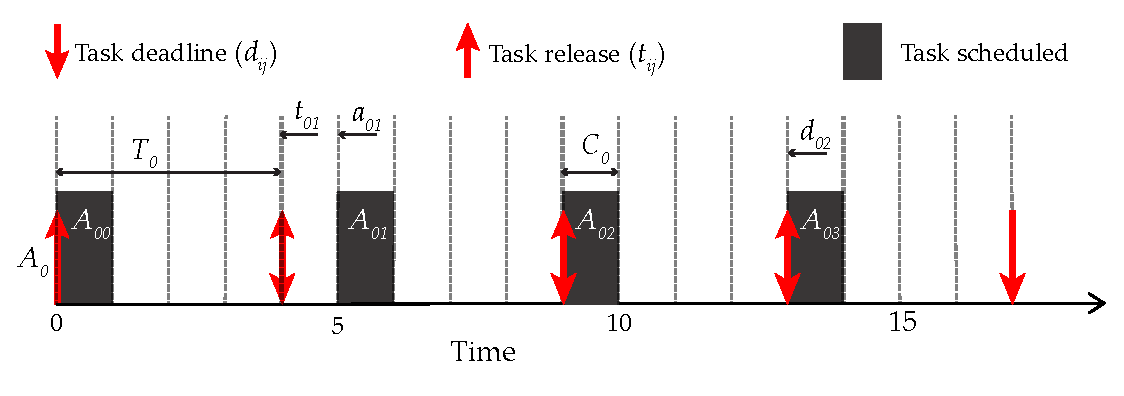
\includegraphics[width=\textwidth]{sporadic}
        \caption{Diagram of the sporadic task model notation described in \cref{t:notation}, showing
        a task set $A$ with a single task $A_{0}$ where $T_{0} = 4$ and $C_{0} = 1$.}
		\label{fig:fp-schedule}
	\end{center}
\end{figure}


\section{Scheduling}
\label{sec:rt-scheduling}
% introduce scheduling terms, how we describe and evaluate schedulers

Simply put, scheduling is deciding which task to run at a specific time. More formally, scheduling
is the act of assigning resources to activities or tasks~\citep{Baruah_CPV_96}, generally discussed
in the context of processing time, but is required for other resources such as communication
channels.  A correct scheduling algorithm  can guarantee that all deadlines are met within their
requirements, whilst also maintaining maximum utilisation of the scheduled resource(s).

Scheduling can be either \emph{static} or \emph{dynamic}. In a static or \emph{off-line} schedule, 
the set of tasks is fixed and the schedule pre-calculated when the system is built, and does not
change once the system is running. 
Dynamic or \emph{on-line} scheduling occurs while the system is running, and the schedule is
calculated whenever a scheduling decision is required. In dynamic systems, the task set can change,
allowing task parameters to be adjusted, and allowing tasks to be added and removed while the system
is running.

A task set is schedulable by a scheduling algorithm if all temporal requirements are satisfied.
If at least one scheduling algorithm can schedule a task set, it is said to be \emph{feasible}.
An \emph{optimal} scheduling algorithm can schedule every feasible task set.
To test if a task set is schedulable by a scheduling algorithm, a \emph{schedulability test} is applied.
The complexity of schedulability tests is important for both dynamic and static schedulers. For
static schedulers, the test is conducted offline and not repeated, but the algorithm must complete
in a reasonable time for the number of tasks in the task set. Dynamic schedulers conduct
schedulability test each time a new task is submitted to the scheduler, or scheduling parameters are
altered, which means the test cannot be too complex to reduce overheads. The schedulability test conducted at admission time is
referred to as an \emph{admission test}.

There is an absolute limit on task sets that are feasible which can be derived from the total
utilisation. 
The \emph{total utilisation} of a task set is the sum of all of the rates and must be less than the
total processing capacity of a system for all deadlines to be met.
For each processor in a system, this amounts to \cref{eq:1}.
\begin{equation}
    \label{eq:1}
	\sum\limits_{i=0}^n \dfrac{C_{i}}{T_{i}} \leq 1
\end{equation}
If the inequality does not hold, the system is considered \emph{overloaded}. Overload
can be \emph{constant}, in that it is all the time, or \emph{transient}, where the overload may be
temporary due to exceptional circumstances.

\begin{table}
    \centering
    \begin{tabular}{cccc} \toprule
        & \emph{$C_{i}$} & $T_{i}$ & $U_{i} $ \\ \midrule
			$ A_{1}$ & 1 & 4 & 0.25 \\
			$ A_{2}$ & 1 & 5 & 0.20 \\
			$ A_{3}$ & 3 & 9 & 0.33 \\
			$ A_{4}$ & 3 & 18 & 0.17  \\\midrule 
	$ U_{sum}(\tau)$ & &  & 0.95 \\ \bottomrule
	\end{tabular}
	\caption{A sample task set, adapted from ~\citep{Brandenburg:phd}}
	\label{tab:example_task_set}
\end{table}

Ideally, task sets are scheduled such that the total utilisation is equal to the number of
processors.  In practice, scheduling algorithms are subject to two different types of \emph{capacity
loss} which render 100\% utilisation impossible---algorithmic and overhead-related.
\emph{Algorithmic} capacity loss refers to processing time that is wasted due to the schedule used,
due to a non-optimal scheduling algorithm.  \emph{Overhead-related} capacity loss refers to time
spent due to hardware effects (such as cache misses, cache contention, and context switches) and
computing scheduling decisions.  Accurate schedulability tests should account for overhead-related
capacity loss in addition to algorithmic capacity loss.

Tasks often do not use all of their execution requirement, any execution remaining in is referred to
as \emph{slack}. For \gls{HRT} tasks, slack is a consequence of pessimistic \gls{WCET} values. Slack
also occurs for \gls{SRT} tasks as they may be variable in length. Slack also occurs for aperiodic
tasks where the actual arrival time varies from the minimum inter-arrival time. Many scheduling algorithms
attempt to gain performance by reclaiming or stealing slack.

Scheduling algorithms are classed as either dynamic or fixed priority. A scheduling algorithm 
is \emph{fixed priority} if all the jobs in each task run at the same priority, which never changes. 
\emph{Dynamic priority} scheduling algorithms assign priorities to jobs not tasked, based on some criteria. 
There are two definitive scheduling algorithms: \gls{FPRM}, which has fixed priorities, and
\gls{EDF}, which has dynamic priorities. Each is optimal for its respective scheduling class,  and both algorithms are defined along with
schedulability tests for the periodic task model in the seminal paper by \citet{Liu_Layland_73}. We
describe them briefly here. 

% survey of scheduling algorithms (FP, EDF, PFAIR)
\subsection{Fixed priority scheduling}
\label{s:fp}

As the name implies, \gls{FP} scheduling involves assigning fixed priorities to each task.
The scheduler is invoked when a job is released or a job ends.
The job with the highest priority is always scheduled.

Priority assignment such that all tasks meet their deadlines is the core challenge of \gls{FP} scheduling.
Two well established techniques are \gls{RM} and deadline monotonic, both of which are optimal with respect to \gls{FP} scheduling.
\Gls{RM} priority assignment~\citep{Liu_Layland_73} allocates higher priorities to tasks with higher
rates---where \emph{rate} is determined by the period, as shown in \cref{eq:2}.
\begin{equation}
    \label{eq:2}
	\dfrac{1}{T_{i}}
\end{equation}

Schedulability analysis for \gls{RM} priority assignment requires that deadlines are equal to periods.
\Gls{DM} priority assignment~\citep{Leung_Whitehead_82} allocates higher priorities to tasks with shorter deadlines and relaxes this requirement.
In both cases, ties are broken arbitrarily.
The \gls{FP} scheduling technique itself is not optimal, as it results in algorithmic capacity loss
and may leave up to 30\% of the processor idle. \cref{eq:3} shows the schedulability test for
\gls{FPRM}, and \cref{eq:4} shows that the limit as the number of tasks in the task set ($n$) tends
towards infinity.
\cref{f:fp-schedule} shows an example \gls{FPRM} schedule.

\begin{equation}
    \label{eq:3}
    \sum\limits_{i=0}^n \dfrac{C_{i}}{T_{i}} \leq n(2^{\frac{1}{n}}-1)
\end{equation}
\begin{equation}
    \label{eq:4}
    \lim_{n \to \infty}n(\sqrt[n]{2}-1) = \ln_{} 2 \approx 0.693147...
\end{equation}

\begin{figure}
	\begin{center}
		\leavevmode
		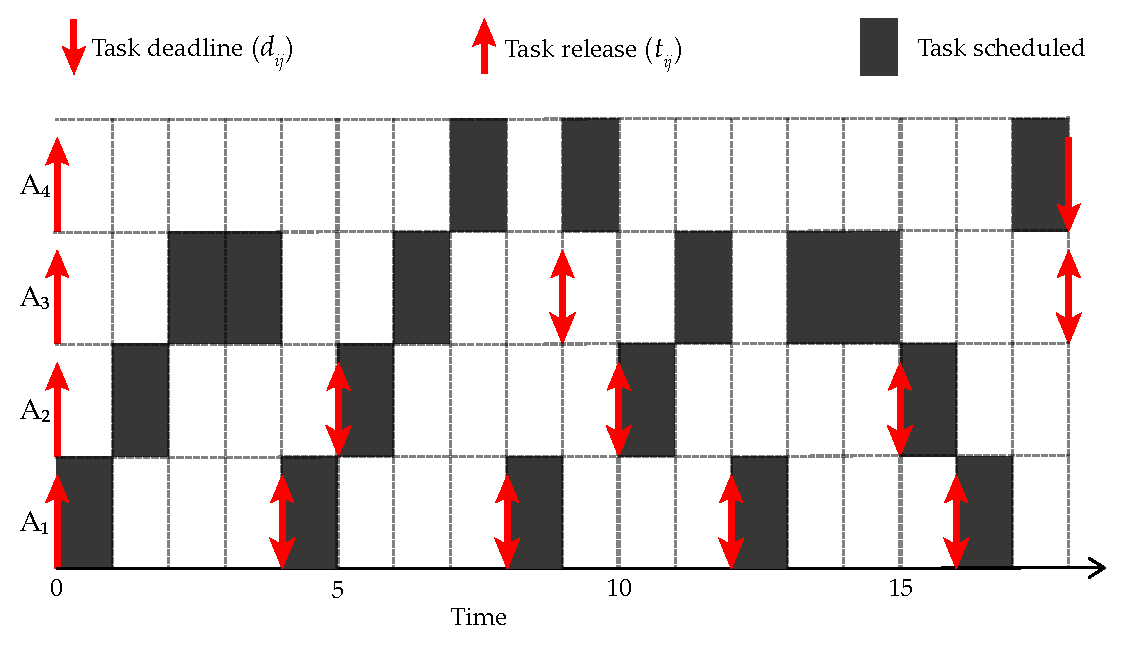
\includegraphics[width=\textwidth]{fpschedule}
		\caption{An example FPRM schedule using the task set from Table \ref{tab:example_task_set}.}
		\label{f:fp-schedule}
	\end{center}
\end{figure}

\subsection{Earliest Deadline First Scheduling}

The \gls{EDF} algorithm is theoretically optimal for scheduling a single resource, with no
algorithmic capacity loss; that is 100\% of processing time can be scheduled. This is because
\gls{EDF} uses dynamic priorities rather than fixed priorities. 
Priorities are assigned by examining the deadlines of each ready job; jobs with more immediate deadlines have higher priorities.
\Cref{f:edf-schedule} illustrates how the task set in \cref{tab:example_task_set} is scheduled by
\gls{EDF}, highlighting the places where tasks are scheduled differently from FPRM.

\begin{figure}
	\begin{center}
		\leavevmode
		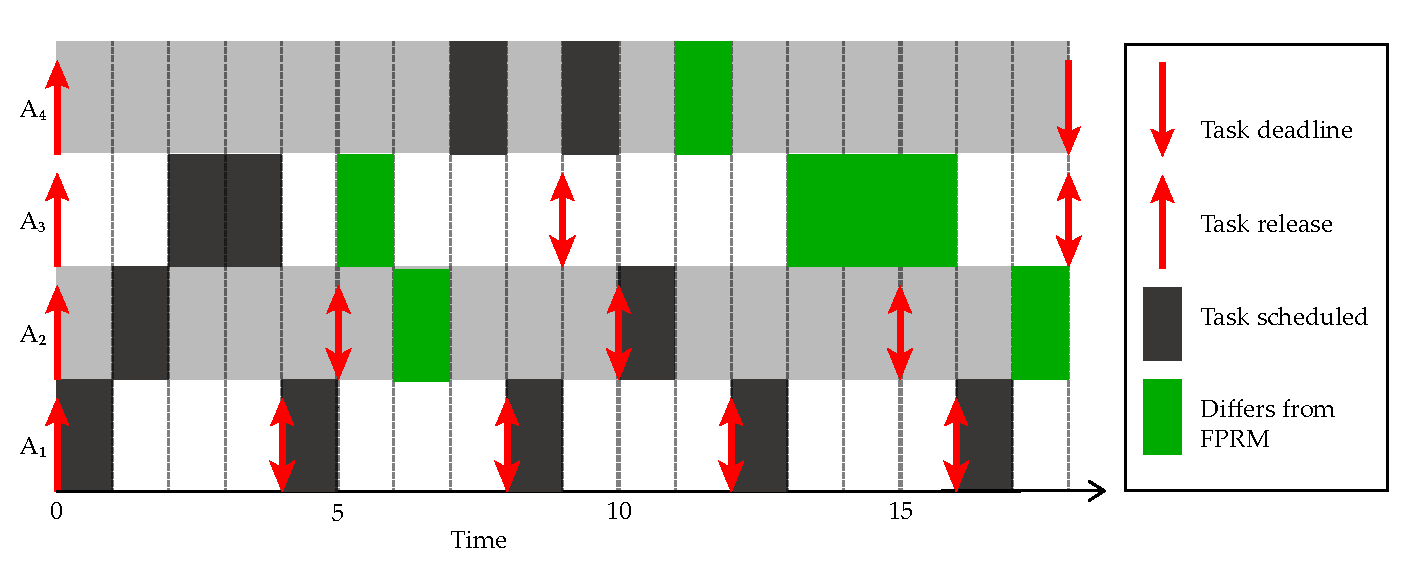
\includegraphics[width=\textwidth]{edfschedule}
		\caption{An example EDF schedule using the task set from Table \ref{tab:example_task_set}.}
		\label{f:edf-schedule}
	\end{center}
\end{figure}

\subsection{Earliest Deadline First vs. Fixed Priority Scheduling}
\label{s:overload}

\gls{EDF} is less popular in commercial practice than \gls{FP} for a number of reasons.  \gls{EDF}
is considered more complex to implement and to have higher overhead-related capacity loss.
Both algorithms have different behaviour under overload, and many consider the \gls{FP} behaviour
preferable. \gls{FP}
is mandated by the POSIX standard, possibly due to these misconceptions. One common argument for
\gls{FPRM} is the idea that the algorithmic capacity loss is mediated by the overhead related
capacity loss of \gls{EDF}, and much easier to implement. 

However, all of these points were debunked by \citet{Buttazzo_05}.  Although \gls{EDF} is difficult
and inefficient to implement on top of existing, priority-based \glspl{OS}, both schedulers
can be considered equally complex to implement from scratch.  \gls{FP} scheduling has higher
overhead-related capacity loss due to an increase in the amount of preemption.  This compounds the
algorithmic capacity loss, rendering \gls{EDF} a clear winner in from-scratch implementations.

Other comparisons between \gls{EDF} and \gls{FP} are the complexity of their schedulability tests.
\gls{EDF} and \gls{FP} scheduling both have pseudo-polynomial
schedulability tests under the sporadic task model, although \gls{EDF} under the periodic task
model\footnote{The periodic task model is the same as the sporadic task model, with the restriction
that deadlines must be equal to periods ($d = p$), while periods themselves are considered absolute,
not minimum.} has an $O(n)$ schedulability test.  Like all pseudo-polynomial problems,
approximations can be made to reduce the complexity, although this comes with an error factor which
may not be suitable for \gls{HRT} systems.  

Both algorithms behave differently under constant
overload. \gls{EDF} allows progress for all jobs but at a lower rate, while \gls{FP} will
continue to meet deadlines for jobs with higher \gls{RM} priorities, completely starving other
jobs. Whether these behaviours are desirable is subject to context.  Under
transient overload conditions both algorithms can cause deadline misses.

% TODO mention reneging?

\subsection{Multiprocessors}

Both fixed and dynamic scheduling algorithms scheduling can be used on multiprocessor machines, either
\emph{globally} or \emph{partitioned}. Global schedulers share a single scheduling data structure
between all processors in the system, whereas partitioned schedulers have a scheduler per processor.
Neither is perfect: global approaches suffer from scalability issues such as hardware contention,
however partitioned schedulers require load balancing across cores.  Partitioning itself is known to
be a NP-hard bin-packing problem.  On modern hardware, partitioned schedulers outperform global
schedulers~\citep{Brandenburg:phd}.  For clustered multiprocessors a combination of global and
partitioned scheduling can be used; global within a cluster, and partitioned across clusters.

\section{Resource sharing}
\label{sec:resource-sharing-theory}

In the discussion so far we have assumed all real-time tasks are separate, and do not share resources.
Of course, any practical system involves shared resources. In this section we introduce the basics
of resource sharing, and the complexities of doing so in a real-time system.

Access to shared resources requires \emph{mutual exclusion}, where only one 
task is permitted to access a resource at a time, to prevent system corruption. Code that
must be accessed in a mutually exclusive fashion is called a \emph{critical section}. Generally
speaking, tasks lock access to resources, preventing other tasks from accessing that resource
until it is unlocked. However many variants on locking protocols exist, including locks that permit
$n$ tasks to access a section, or locks that behave differently for read and write access.

Resource sharing in a real-time context is more complicated than standard resource sharing and
synchronisation, due to the problem of \emph{priority inversion}, which threatens the temporal
correctness of a system.  Priority inversion occurs when a low priority task prevents a high
priority task from running.  Consider the following example: if a low priority task locks a resource
that a high priority task requires, then the low priority task can cause the high priority task to
miss its deadline.  Consequently, all synchronised resource access in a real-time system must be
bounded, and the deadlines of tasks must account for those bounds.

Bounded critical sections alone are not sufficient to guarantee correctness in a real-time
system. Consider the scenario outlined earlier, where a low priority thread holds a lock that a high
priority thread is blocked on.  If other, medium-priority tasks exist in the system, then the low
priority task will never run and unlock the lock, leaving the high priority task blocked for an
unbounded period.  This exact scenario caused the Mars Pathfinder to fault, causing unexpected
system resets~\citep{Mars_Pathfinder}.

In this section we provide a brief overview of real-time synchronisation protocols that
avoid unbounded priority inversion, drawn from \citet{Sha_RL_90}. First we consider uniprocessor
protocols before canvassing multiprocessor resource sharing.

\subsection{Non-preemptive critical sections}

Using the \gls{NCP}, preemption is totally disabled whilst in a critical section.  This approach blocks
all threads in the system while any client accesses a critical section.  Consequently, the bound on
any single priority inversion is the length of the longest critical section in the system.  Although
functional, this approach results in a lot of unnecessary blocking of higher priority threads.  The
maximum bound on priority inversion that a task can experience is the sum of the length of all
critical sections accessed by that task. 
\TODO{Explain how the maximum priority bound is deduced}

\subsection{Priority Inheritance Protocol}
\label{sec:pip}

In the \gls{PIP}, when a high priority task encounters a locked resource, it donates its priority 
to the task holding the lock. When the lock is released the priority is restored. 
This approach avoids blocking any higher priority threads that do not access this resource, and
works for both fixed and dynamic priority scheduling.
However, \gls{PIP} results in a large preemption overhead and as a result has poor WCET analysis.

To understand this, consider a task set with $n$ tasks, $A_{1}, ... , A_{n}$, where each task's priority
corresponds to its index, such the priority of $A_{i} = i$. The highest priority is $n$ and the
lowest is 1 and all tasks access the same resource. If $A_{1}$ holds the lock to that resource, then
the worst preemption overhead occurs if $A_{2}$ wakes up, elevating the priority of $A_{1}$ to 2. Subsequently,
each task wakes up in increasing priority order, each preempting $A_{1}$ until its priority reaches
$n$ resulting in $n$ total preemptions. 

Another disadvantage of \gls{PIP} is that deadlock can occur if resource ordering is not used.


\subsection{Immediate Priority Ceiling Protocol}
\label{sec:hlp}
\label{sec:ipcp}

Under \gls{IPCP}, also known as the highest lockers protocol, resources are assigned a
\emph{ceiling} priority: the highest priority of all tasks that access that resource + 1.  When tasks
lock that resource, they run at the ceiling priority, removing the preemption overhead
of \gls{PIP}.

The disadvantage of \gls{IPCP} is that all priorities of task that access locked resources must be known \emph{a
priori}.  Additionally, if priority ceilings are all set to the highest priority, then behaviour
degrades to that of \gls{NCP}. Finally this protocol allows intermediate priority tasks that do not need
the resource to be blocked. 

\subsection{Original Priority Ceiling Protocol}

The \gls{OPCP} combines the previous two approaches, and avoids deadlock, excessive blocking and
excessive preemption. In addition to considering the priorities of tasks, \gls{OPCP} introduces
a dynamic global state referred to as the \emph{system ceiling}, which is the highest
priority ceiling of any currently locked resource. When a task locks a resource, its priority 
is not changed until another task attempts to acquire that resource, at which point the resource
holder's priority is boosted to the resource's ceiling. By delaying the priority boost the excessive 
preemption of \gls{PIP} is avoided. Additionally, tasks can only lock resources
if when priority is higher than the system ceiling, otherwise they block until this condition is
true, thus avoiding the risk of deadlock. \gls{OPCP} results in less blocking overall than \gls{IPCP},
however requires global state to be tracked across all tasks, even those that do not share
resources, increasing the complexity of an implementation.

Neither protocol requiring resource ceilings is suitable for dynamic priority scheduling algorithms
like \gls{EDF}, however analogous algorithms exist, namely the \gls{SRP}~\citep{Baker_91}.

\subsection{Other locking protocols}

We do not consider lock-free and wait-free algorithms in detail in this chapter, but note while
these may be deployed in real time systems there are always resources that need true blocking in
order to access them; in a word, stateful devices. For memory based resources, there is no need for 
algorithms that avoid blocking, as long as the total blocking time is bounded 
and fairness is not mandated. Any approach that is 
transactional with no guarantee of progress is not suitable, additionally, fair algorithms are not suited to a
real-time system, which are fundamentally not fair. 

\subsection{Summary}

\begin{figure}[ht]
  \centering
  \setlength{\unitlength}{1mm}
  \begin{picture}(50,25)(-5,-5)
    % WHOA! My first use of the picture environment in 25 years ;-)
    \thicklines
    \put(-5,0){\vector(1,0){50}}
    \put(7,-4){Priority inversion bound}
    \put(0,-5){\vector(0,1){25}}
    \put(-4.5,2){\rotatebox{90}{Complexity}}
    \put(2,15){OPCP}
    \put(12,3){IPCP}
    \put(25,11){PIP}
    \put(35,1.5){NCP}
  \end{picture}
  \caption{Comparison of real-time locking protocols based on
    implementation complexity and priority inversion bound.}
  \label{f:locking}
\end{figure}

\Cref{f:locking} compares the different uniprocessor locking protocols, showing that \gls{OPCP}
provides the lowest bound on priority inversion; however is also the most complicated to implement.
\gls{NCP} on the other hand, is the simplest to implement but exhibits the worst priority inversion
behaviour, with \gls{PIP} and \gls{IPCP} falling between the two.  \gls{IPCP} provides minimal
implementation complexity but requires a policy on priority assignment to be in place in the system.

\subsection{Multiprocessor locking protocols}

Resource sharing on multiprocessors is far more complicated than the single processor case and still
a topic of active research. Of course, uniprocessor techniques can be used for resources that are
local to a processor, but further protocols are required for resources shared across cores (termed
\emph{global} resources).

Protocols for multiprocessor locking are either spinning- or suspension-based;
\emph{spinning} protocols spin on shared memory; \emph{suspension} protocols block the
task until the resource is available, such that other tasks can use the processor during that time.
Spin-lock protocols are effective for short critical sections, but once the critical section exceeds
the time taken to switch to another task and back, semaphore protocols are more efficient. 

Multiprocessor locking protocols differ depending on the scheduling policy across cores; in
partitioned approaches, priorities on different cores are not comparable, meaning existing protocols
do not work. While the protocols we have examined so far can be used under global scheduling,
\citet{Brandenburg:phd} showed that partitioned approaches suffer far less cache overheads than
global scheduling. 

The \gls{MPCP}~\citep{Rajkumar_90} is a modified version of \gls{OPCP} for multiprocessors. It is a
suspension-based protocol that works by boosting task priorities. Tasks run at the highest priority
of any task that may access a global resource, and waiting tasks block in a priority queue. Nested
access to global resources is disallowed. The \gls{MSRP}~\citep{Gai_DL_03} is a spin-lock based
protocol, which can be used for \gls{FP} and \gls{EDF} scheduling. \gls{MSRP} uses the \gls{SRP} locally,
combined with \gls{FIFO} spin-locks which guard global resources. 

Multiprocessor real-time locking protocols are an extensive field of research, and 
many more sophisticated locking protocols exist, however we do not survey them here.

\section{Mixed-criticality systems}
\label{s:mixed-criticality}

Broadly, a mixed-criticality system is simply a system where software classified at different levels
of criticality, according to a standard such as DO-178C (recall \Cref{tab:criticality_table}), share
the same physical hardware. 

\TODO{references in this paragraph}
Varying definitions exist in the literature. Some consider merely
the combination of \gls{HRT}, \gls{SRT} and best effort tasks, with criticality observed in that order.
Others allow for \gls{QoS} specifications, which can reflect criticality. 

In the real-time community, much work has been
conducted around a theoretical model introduced by \citet{Vestal_07}. In this model, a system has
a specific range of criticality levels, $L_{min} - L_{max}$ and a current criticality level
$L_{now}$. Each task in the system is assigned a criticality level, $L_{i}$, and has a vector of
execution times of size $L_{i} - L_{min}$. When the system undergoes a mode change, should $L_{i}
\leq L_{now}$ the execution time required by that task is set to the value in the vector
corresponding to the new $L_{now}$. If a tasks criticality is less than $L_{now}$, it may be dropped
or scheduled with much lower priority until a mode switch increases $L_{now}$. 

This model can be interpreted in several ways; as a form of graceful degradation; or as an
optimisation in the case where a system designer and \gls{CA} disagree on \gls{WCET}
estimates for a system. Theoretically, if the system designer could show that the higher estimates
of the \gls{CA} can be met by such a mode change, they could schedule less criticality tasks when in
a low criticality mode. 

However, while this model, and many variations upon it have been subject to much research in the
real-time community, questions have been raised as to its practicality in industry.
\citet{Ernst_DiNatale_16} claim that a \gls{CA} would be unlikely to accept multiple \gls{WCET}
definitions and state that the focus of mixed-criticality research should be on providing systems
for error handling and proof of isolation in order to make mixed-criticality systems practical. 

The focus on this thesis is for the broader definition of mixed-criticality, such that software of
different levels of criticality can safely share hardware, and not specifically the model
presented by \citet{Vestal_07} and beyond~\citep{Burns_Davis_17}.

\section{Operating systems}
\label{sec:background-operating-systems}

An \gls{OS} is a software system that interfaces with hardware and devices in order to present a
common interface to applications.  The \emph{kernel} is the part of the operating system that
operates with privileged access to the processor(s) in order to safely perform tasks that allow
applications to run independently of each other.

Common \glspl{OS}, such as Windows, MacOS and Linux, are \emph{monolithic} operating systems,
which means that many services required to run applications are inside the kernel.  A \emph{microkernel}
attempts to minimise the amount of code running in the kernel in order to reduce the amount of
trusted code.  Figure \ref{fig:os-microkernel} illustrates the difference between monolithic
\glspl{OS} and microkernels.  Modern microkernel implementation is guided by the minimality
principle~\citep{Liedtke_95} which aims to provide minimal mechanisms to allow resource servers to
function, leaving the rest of the policy up to the software running outside of the kernel. According
to the minimality principle, if a service does not need to be in the kernel to achieve its'
functionality, it should not be in the kernel.

\begin{figure}[tb]
	\begin{center}
		\leavevmode
		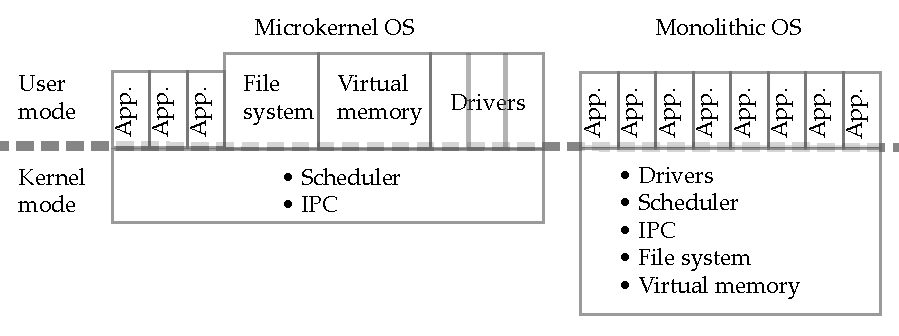
\includegraphics{os-microkernel.pdf}
		\caption{Structure of a microkernel vs. monolithic operating system.}
		\label{fig:os-microkernel}
	\end{center}
\end{figure}

Monolithic operating systems provide scheduling, \gls{IPC}, device drivers, memory allocation, file
systems and other services in the kernel, resulting in a large \emph{trusted computing base}.
Interpretations of the minimality principle varies, 
consequently which services and utilities are included in the privileged kernel varies. In
larger kernels thread scheduling, memory allocation and some device drivers are included in the kernel.
For example, \selfour~\citep{Klein_EHACDEEKNSTW_09} contains a scheduling, \gls{IPC}; 
\composite~\citep{Parmer:phd} does not provide a scheduler. 

Microkernels are far more amenable for deployment in areas where security is a primary concern,
due to their small trusted computing base.
Services on top of the microkernel can be isolated and assigned different levels of trust, unlike
the services in a monolithic \gls{OS} which all run at the same privilege level such that a fault in
one service can compromise the entire system. 

\subsection{Capabilities}

Many security-focused microkernels make use of \emph{capabilities}~\citep{Dennis_VanHorn_66}, an
established mechanism for fine-grained access control to spatial resources which allow for spatial
    isolation. A capability is a unique, unforgeable token that gives the possessor permission to access
an entity or object in system. Capabilities can have different levels of access rights, e.g. read,
write, execute etc. 

By combining access rights with object identifiers capabilities avoid the
confused deputy problem, a form of privilege escalation where a deputy program
acting on behalf of a client is  tricked into using
its own rights to manipulate a resource that the client would not normally have access
to~\citep{Hardy_88}. 

\subsection{IPC}
\label{s:background-ipc}

\gls{IPC} is the microkernel mechanism for synchronous transmission of data and capabilities between
processes. Because the microkernel model provides services encapsulated into user-level servers,
\gls{IPC} is key to microkernel performance, as it is used for more predominantly than in monolithic
\glspl{OS}. Originally, microkernels were criticised as impractical due to inefficient IPC
implementations, however this was demonstrated to be false~\citep{Hartig_HLSW_97} with the
development of very fast microkernels with optimised code paths for IPC, referred to as \emph{fastpaths}. 


\subsection{Open vs. Closed Systems}

Operating systems can be built for open or closed systems.  An \emph{open system} is any system
where code outside of the control of the system designers can be executed. For example, modern
smart phones are open systems, given that users can install third-party applications.

A \emph{closed system} is the opposite; the system designers have complete control over all code
that will execute on the system.  The majority of closed systems are embedded, including those found
in cars, spacecraft and aircraft.

In general, there is a trend toward systems becoming more open; initial mobile phones were closed
systems.  This trend can be perceived from infotainment units in automobiles to televisions, where
the option to install third party applications is becoming more prevalent.  Allowing third-party
applications to run alongside critical applications on shared hardware increases the security
requirements of the system: critical applications must be isolated from third-party applications and
secure communications must be used between distributed components.  This is currently not the
general case, which has led to researchers demonstrating attacks on
cars~\citep{Checkoway_MKASSKCRK_11}.

Open systems are generally \emph{dynamic}---where resource allocations are configured at run-time
and can change---as opposed to closed systems which have \emph{fixed} or \emph{static} resource
allocation patterns.

%% introduce RTOSes
\subsection{Real-Time Operating Systems}

A \gls{RTOS} is an \gls{OS} that provides temporal guarantees, and can be microkernel-based or
monolithic.  Whilst some real-time systems run without operating systems at all, this approach is
generally limited to small, closed systems and is both inflexible and difficult to
maintain~\citep{Lui_AACBBBCLM_04}.

In a general purpose \gls{OS}, time is shared between applications with the aim of providing
\emph{fairness}, where applications share the processor equally.  This fairness is not divided into
equal share, but weighted, such that some applications are awarded more time than others in order
to tune overall system performance.  The \gls{OS} itself is not directly aware of the timing needs of
applications.

In an \gls{RTOS}, fairness is replaced by the need to meet deadlines. As a result, time is promoted
to a first class resource~\citep{Stankovic_88}.

Time being an integral part of the system affects every other part of the \gls{OS}.  For example, in
an \gls{RTOS}, one application having exclusive access to a resource cannot be allowed to cause a
deadline miss.  Similarly, the \gls{RTOS} itself cannot cause a deadline miss.  This means that all
operations in the \gls{RTOS} must either be bounded with known {\gls{WCET}} or the \gls{RTOS} must
be fully preemptible.  However, it must be noted that a fully preemptible \gls{OS} is completely
non-deterministic, making correctness impractical to guarantee~\citep{Blackham_TH_12}.  The overheads
of \gls{RTOS} operations like interrupt handling and context switching must also be considered when
determining whether deadlines can be met.

Traditional \glspl{RTOS}, and the applications running on them, require extensive offline analysis
to guarantee that all temporal requirements are met.  This is done by using scheduling algorithms,
\gls{WCET} analysis, and resource sharing algorithms with known real-time properties.

\subsection{Resource kernels}
\label{sec:resource-kernels}

Resource kernels are a class of \gls{OS} that treat time as a first class resource, by providing
timely, guaranteed access to system resources.  In a resource kernel, a reservation represents a
portion of a shared resource, like processor, or disk bandwidth.  Unlike traditional real-time
operating systems, resource kernels do not trust all applications to stay within their specified
resource bounds: resource kernels enforce them, preventing misbehaving applications from interfering
with other applications and thus providing temporal isolation.

In the seminal resource kernel paper, \citet{Rajkumar_JMO_98} outline four main goals that are
integral to resource kernels:
\begin{description}
    \item[G1: Timeliness of resource usage] Applications must be able to specify resource
        requirements that the kernel will guarantee.  Requirements should be dynamic: applications
        must be able to change them at run-time, however the kernel should ensure that the set of
        all requirements can be admitted.
    \item[G2: Efficient resource utilisation] The mechanisms used by the resource kernel utilise
        available resources efficiently and must not impose high utilisation penalties.
    \item[G3: Enforcement and protection] The kernel must enforce resource access such that rogue
        applications cannot interrupt the resource use of other applications.
    \item[G4: Access to multiple resource types] The kernel must provide access to multiple resource
        types, including processing cycles, disk bandwidth, network bandwidth and virtual memory.
\end{description}

In another paper, \citet{deNiz_LSR_01} outline the four main mechanisms that a resource kernel must
provide, in order to implement the above concepts.

\begin{description}
	\item[Admission] check that all resource requests can be scheduled (\textbf{G1}).
	\item[Scheduling] implements the dynamic allocation of resources according to reservations (\textbf{G1, G2}).
	\item[Enforcement] limit the consumption of the resources to that specified by the reservation(\textbf{G3}.
	\item[Accounting] of reservation use, to implement scheduling and enforcement (\textbf{G1, G2, G3}).
\end{description}

In order to share resources in a resource kernel, avoiding priority inversion becomes a more
complicated problem.  \citet{deNiz_LSR_01} outline three key policies that must be considered when
handling resource sharing in reservation-based systems:

\begin{description}
    \item[Prioritisation] What (relative) priority is used by the task accessing the shared resource (and under what conditions)?
    \item[Charging] Which reservation(s), if any, gets charged, and when?
    \item[Enforcement] What happens when the reservations being charged by the charging policy expire?
\end{description}

Resource kernels are a form of monolithic operating system, where all system services and drivers
are provided by the kernel.  In a microkernel, not all of the mechanisms of a resource kernel are
suitable for inclusion in the kernel itself: some can be provided by user-level middle-ware.  This
is because core resource kernel concepts contain both policy and mechanism.  We argue that the
microkernel should provide resource kernel mechanisms such that a resource kernel can be built with
a microkernel, but policy should be left up to the system designer, as long as it does not result in
performance or security concessions.

\section{Summary}

In this chapter we have briefly covered the core real-time theory that this thesis draws upon.
We have defined operating systems, and introduced the concepts that inform the design of resource kernels.
In the next chapter we will survey how these can be combined to achieve isolation and asymmetric protection for mixed-criticality systems.

\chapter{Temporal Isolation \& \\ Asymmetric Protection}
\label{chap:scheduling}

Mixed-criticality systems at their core require isolation: isolation as strong as that provided by
physically isolated systems, meaning if one system fails it cannot effect another system.  Isolation
can be divided into two categories of resources; physical and temporal. Physical resources include 
devices and memory, where isolation can be achieved using the \gls{MMU} and \IO\glspl{MMU}.
Temporal isolation of resources more complicated, and is our focus in this chapter, where
we survey the relevant literature.
A system is said to provide \emph{temporal isolation} if temporal faults in one task cannot cause
temporal faults in another, independent task. 

However, what does isolation mean in a fully or over-committed system, where there is no slack time 
to schedule? What if there simply is not enough time? One might argue that the method of
over-provisioning systems in order to never face such a scenario is sufficient and should not be
changed. However, in the presence of \gls{SRT} and best-effort tasks which may be low in
criticality, this requirement is too strong. Instead we must explore mechanisms for \emph{asymmetric
protection}, where high criticality tasks can cause a failure in low criticality tasks, but not vice
versa.

Much of the background examined in the previous chapter (\cref{sec:real-time-theory})
made the assumption that tasks would not exceed a declared \gls{WCET} or critical section bound. 
Many existing real-time systems run either one application, or multiple applications of the same
criticality, meaning each application that is running is certified to the same level.  This means
that all applications are trusted: trusted to not crash, and trusted to not overrun their deadlines.
If one application does overrun its deadline or use more processing time that specified by its
\gls{WCET}, guarantees are no longer met. 

The issue of trust in real-time literature has not been greatly addressed: real time tasks are often
assumed to perform correctly and safely.  However, much research has looked into the scheduling of
aperiodic tasks, which by definition do cannot be trusted to follow a specific schedule, or abide by
their estimated minimum inter-arrival time. Further applicable research examines the scheduling of
\gls{SRT} and best-effort tasks along with \gls{HRT} tasks. Consequently we examine scheduling methods for
these types of systems. 

Neither \gls{FP} or \gls{EDF} scheduling
approaches discussed so far provides temporal isolation, although both can be adapted to do so.  In
this chapter we examine the techniques used by the real-time community to achieve temporal
isolation.

% TODO we should consider asymmetric protection here?
% TODO this sounds like it belongs in the chapter summary
%Temporal isolation requires tasks to specify their expected, or permitted temporal behaviour. This
%can be done by specifying a processor share, as in proportional share schedulers, or by using the
%period and execution requirement of the sporadic task model as an upper bound on task processor
%utilisation.

\section{Scheduling}

% TODO intro here

\subsection{Proportional share schedulers}

Proportional share schedulers provide temporal isolation, as long as the system is not overloaded,
although this class of schedulers is based on achieving scheduling fairness between tasks, rather
than running untrusted tasks which may exceed their execution requirement. 

Recall that fairness is not a central property of scheduling in an \gls{RTOS}. However, one approach
for real-time scheduling is to specify a set of constraints that attempt to provide fairness and
also satisfy temporal constraints.  These are referred to as \emph{proportional share} algorithms,
which allocate time to tasks in discrete sized quanta. Tasks in proportional share schedulers are assigned 
weights according to their rate, and those weights determine the share of time for which each task 
has access to a resource.

While proportional share algorithms are applied to many different scheduling problems, they apply
well to real-time scheduling on one or more processors.
Unlike other approaches to real-time scheduling, proportional share schedulers have the explicit property of guaranteeing a rate of progress for all tasks in the system.

\citet{Baruah_CPV_96} introduced the property \emph{proportionate fairness} or \emph{Pfair} as a
strong fairness property for proportionate share scheduling algorithms.  For a schedule to be Pfair,
then at every time $t$ a task $T$ with weight $T_{w}$ must have been scheduled either $\lceil T_{w}
. t \rceil$ or $\lfloor T_{w}.t \rfloor $ times.  \emph{Early-Release fair} or
ERfair~\citep{Anderson_Srinivasan_04} is an extension of the Pfair property that allows tasks to
execute before their Pfair window, which can allow for better response times.

Pfair scheduling algorithms break jobs into sub-jobs that match the length of a quantum.
Real-time and non-real time tasks are treated similarly.
When overload conditions exist, the rate is slowed for all tasks.

Pfair scheduling algorithms are good theoretically but do not perform well in practice; they incur
large overhead related capacity loss due to an increased number of context
switches~\citep{Abeni_Buttazzo_04}. Additionally, since
scheduling decisions can only be made at quantised intervals, scheduling is less precise in
proportionate fair systems.  This problem can be exacerbated by critical sections, which may last
longer than a single quantum.  \citet{Stoica_AKBGP_96} propose defining arbitrary quanta sizes based
on maximum critical section size, however quanta size decreases the accuracy of the scheduler.
Additionally, it may not be possible to have \emph{a priori} knowledge of critical section size, especially
in a soft real-time systems where it is not worth conducting \gls{WCET} analysis or execution time
is dependant on exterior factors, such as network behaviour.

One early uniprocessor Pfair scheduling algorithm is earliest eligible deadline first, presented in
\citet{Stoica_AKBGP_96}.  PD$^{2}$~\citep{Srinivasan_Anderson_06} is a more recent Pfair/ERfair
scheduling algorithm that is theoretically optimal for multiprocessors under \gls{HRT} constraints,
although only under the assumption that process preemption and migration are free.

Recall that temporal isolation means that tasks should not be able to interfere with the temporal
behaviour of other tasks in the system.  Proportionate fair systems provide temporal isolation as
part of their fairness property, unless the system is overloaded, at which point the rate of all
tasks will degrade. Pfair schedulers by definition do not support asymmetric protection.

\subsection{Isolation with EDF schedulers}

Temporal isolation in \gls{EDF} scheduling has been explored thoroughly in the real-time discipline.
We outline the most dominant approaches in this section.

\paragraph{Robust earliest deadline scheduling}
One early approach to temporal isolation with \gls{EDF} scheduling attempts to extend the 
algorithm to allow overload conditions to be handled with respect to a value. Robust earliest deadline
scheduling~\citep{Buttazzo_Stankovic_93} assigns a value to each task set, and drop jobs from
low-value tasks under overload. If the system returns to non-overload conditions those tasks are
scheduled again. This is a very early version of asymmetric protection
The algorithm is optimal, however this is only the case if
scheduler overhead is excluded.  Since the algorithm is has O($n$) complexity in the number of
tasks, the authors recommend using a dedicated scheduling processor such that overhead will not
effect the timing behaviour -- but this is not suitable for embedded systems, where the goal is to
minimise the number of processors, not increase them.

\paragraph{\Gls{CBS}} \citet{Abeni_Buttazzo_04} introduce a technique for scheduling \gls{HRT} and
\gls{SRT} tasks and providing temporal isolation.  \gls{HRT} tasks are scheduled using an \gls{EDF}
scheduler, but \gls{SRT} tasks are treated differently as \gls{EDF} does not handle overload.
Instead, a \gls{CBS} is assigned to each \gls{SRT} task.  Each \gls{CBS} has a bandwidth assigned to
it, and breaks down \gls{SRT} jobs into sub-jobs such that the utilisation rate of the task does not
exceed the assigned bandwidth.  Any sub-job that will cause the bandwidth to be exceeded is
postponed, but still executed.

\gls{CBS} stands out from previous server based approaches~\citep{Spuri_Buttazzo_96,
Ghazalie_Baker_95, Spuri_Buttazzo_94, Deng_Liu_97} as it does not require a \gls{WCET} or a minimum
bound on job inter-arrival time, making it much more suitable for \gls{SRT} tasks.  Implementation
wise, \gls{CBS} has fewer hardware overheads than Pfair schedulers.

Many extensions exist to \gls{CBS} to improve functionality.  \citet{Kato_IR_11} extend \gls{CBS} to
implement \emph{slack donation}, where any unused bandwidth is given to other jobs.  In
~\citep{Craciunas_KPRS_12}, \gls{CBS} is extended such that bandwidths are variable at run-time.
\citet{Lamastra_LA_01} introduce bandwidth inheritance across CBS servers applied to different
resources, providing temporal isolation for additional resources other than processing time.

\paragraph{\Gls{RBED}} schedulers explicitly separate the resource allocation and dispatching
(choosing which thread to run) in order to provide flexibility in timeliness requirements supported
by the scheduler.  \Gls{RBED} ~\citep{Brandt_BLB_03} is an algorithm that implements such a
scheduler.  In \gls{RBED}, tasks are considered as either \gls{HRT}, \gls{SRT}, best effort or
rate-based.  Tasks are modelled using an extension of the periodic task model, allowing any job of a
task to have a different period.  If rate-based or \gls{HRT} tasks cannot be scheduled at their
desired rate they are rejected.  \gls{SRT} tasks are given their rate if possible with the option to
provide a quality of service specification.  Processor time reservations can be used to make sure
best effort tasks are allowed some execution time.  Otherwise they are allocated slack time unused
by SRT and HRT tasks.  Either way, best effort tasks are scheduled by assigning them a rate that
reflects how they would be scheduled in a standard, fair, quantum-based scheduler.  Based on the
rates used, \gls{RBED} breaks tasks down and feeds them to an \gls{EDF} scheduler to manage
processing time.  Rates are enforced using a one-shot timer to stop tasks that exceed their
{\gls{WCET}}.  As tasks enter and leave the system, the rates of \gls{SRT} tasks will change.  Slack
time that occurs as a result of tasks completing before their deadlines is only donated to best
effort tasks, although the authors note that extensions should be able to donate slack to \gls{SRT}
tasks as well.  \Gls{RBED} is similar to the concept of CBS, however it deals with separate types of
real-time tasks more explicitly.

\subsection{Isolation with FP schedulers}
\label{background:fp-isolation}

While \gls{CBS} and \gls{RBED} provide temporal isolation for \gls{EDF} scheduling, we will now
examine methods for temporal isolation in fixed-priority systems, whilst maintaining compatibility
with rate-monotonic schedulability tests.  Like \gls{CBS}, tasks are constrained by encapsulating
one or more tasks in a server which prevents the task(s) from overrunning their assigned scheduling
parameters.

\paragraph{Polling servers}\label{p:polling-servers}~\citep{Lehoczky_LS_87} wake every period,
checks if there are any pending tasks and runs them for maximum their budget time. If there is no
task to run, the polling server will go back to sleep. That is, at time $t_{i}$, if there are no
tasks ready to execute, the server will sleep until $t_{i+1}$. This has the limitation task latency
is a function of the period $T$.

\paragraph{Deferrable Servers} Unlike polling servers, \emph{deferrable
servers}\citep{Lehoczky_LS_87, Strosnider_LS_95} preserve any unused budget across periods, although
the budget can never be exceeded.  This removes latency problems with polling servers, but
unfortunately breaks rate-monotonic schedulability analysis, as this policy can result in servers
executing back-to-back and exceeding their allocated scheduling bandwidth for any specific occurrence of
the period.  This occurs as deferrable servers replenish the budget to full at the start of each
period, and the budget can be used at any point during a tasks execution. 

We demonstrate the problem with deferrable servers using the notation introduced in
\Cref{t:notation}. Consider a sporadic task with implicit deadlines in a task set, 
$A_{1}$, with jobs $A_{11}, A_{12}, ..., A_{1n}$. Each job in that task set has a deadline once the
period has passed: $d_{1j} = t_{1j} + T_{1}$. The problem occurs if the first job arrives at $a_{11}
= d_{11} - C_{1}$, such that it is only complete at exactly the implicit deadline.  
Then a second job may arrive arrives at the release time $d_{11}$ such that it runs back-to-back with the first
task, from $a_11$ to $d_{11} + C_{1}$, then the task has exceeded its permitted utilisation 
($\frac{C_{1}}{T_{1}})$. As a result deadline misses can be caused in other
tasks, violating temporal isolation.

\paragraph{Sporadic servers}~\citep{Sprunt_SL_89a}\label{p:sporadic} address the problems of
deferrable servers by scheduling multiple replenishment times, in order to preserve the property
that for all possible points in time $U_{i} \leq \frac{C_{i}}{T_{i}}$, known as the \emph{sliding window} constraint, which
is the condition that deferrable servers violate.  Each time a task is preempted, or blocks, a
replenishment is set for current time + $T_{i}$, for the amount consumed.  When no replenishments are
available, sporadic servers have their priority decreased below any real-time task.  The priority is
restored once a replenishment is available.  While this addresses the problems of deferrable
servers, the implementation is problematic as the number of times a thread is preempted or blocked
is potentially unbounded.  It is also subject to capacity loss as tasks that use very small chunks
of budget at a time increase the interrupt load.  The bigger the bound on replenishments the less
accurate the sporadic server, but the more memory used resulting in degraded performance.

\paragraph{Priority exchange servers}~\citep{Sprunt_SL_89a} swap the priority of an inactive
aperiodic task with a periodic task, such that server capacity is not lost but used at a lower
priority.  Implementations of priority exchange require control and access to priorities across an
entire system.

\paragraph{Slack stealing}~\citep{Ramos_Thuel_Lehoczky_93} is an approach that runs a scheduling
task at the lowest priority and tracks the amount of slack per task in the system.  As aperiodic
tasks arrive, the slack stealer calculates whether they can be scheduled or not based on the slack
in the system and current load of periodic tasks.  This method does not provide guarantees at all
for the aperiodic tasks, unless a certain bound is placed on the execution of periodic tasks.

\section{Mixed-criticality schedulers}

In this section, we briefly consider schedulers designed specifically for mixed-criticality systems. 
However, as this has been a very active topic, we refer the reader to \citet{Burns_Davis_17} for
an extensive background. 

Temporal isolation in mixed-criticality systems can result in \emph{criticality inversion}, where
high criticality tasks miss their deadlines due to lower criticality tasks.  Rather than temporal
isolation, mixed-criticality systems require \emph{asymmetric protection}, where deadline misses of
low-criticality tasks caused by high-criticality tasks are permitted, but not vice-versa.  This can
be realised as a system mode-switch or form of graceful degradation.

A key observation about mixed-criticality systems is neither the strictness of the real-time model,
nor rate-monotonic priorities have any direct correlation with the criticality of a task.  While in
general critical tasks are \gls{HRT}, it is possible to have critical tasks that are \gls{SRT}, for
instance, object tracking algorithms whose \gls{WCET} depends on factors external to the software
system.

None of the scheduling algorithms so far directly support mixed-criticality systems.  \gls{RBED} is
the closest, although it assumes a direct relationship between criticality and real-time model, with
the assumption that \gls{HRT} tasks are more critical than \gls{SRT} tasks which are more critical
than best effort tasks. 

Recall that in this model \glspl{CA} provide \gls{WCET} estimates that must be schedulable, however they are often very
pessimistic.  This results in a tasks with two {\gls{WCET}} estimates, one very pessimistic one from
the \gls{CA} and a less pessimistic one from the system designers or automated tools.  As a result
of this, a family of mixed-criticality schedulers exists that handle high criticality tasks with two
{\gls{WCET}} estimates, and low-criticality tasks.  The scheduling algorithm will always schedule
high-criticality tasks.  If high-criticality tasks finish before the lower \gls{WCET} estimate,
lower criticality tasks are also scheduled.  Otherwise, tasks of lower criticality may not be
scheduled at all. 

Schedulers in this class are distinguished by a mode-switch between two or more criticality levels,
which may result in low criticality tasks being dropped or de-prioritised in some way. 
Schedulers for this model of mixed-criticality have been developed and extensively studied for
\gls{FP}~\citet{Vestal_07, Pathan:phd}, \gls{EDF}~\citet{Baruah_BDMVS_11},

\subsection{Zero Slack Scheduling}

\Citet{deNiz_LR_09} propose a scheduling approach that can handle multiple levels of criticality,
called \gls{ZS} scheduling. \gls{ZS} scheduling is based on the fact that tasks rarely use their
\gls{WCET}.  This means that resource reservation techniques like \gls{CBS} without slack donation
result in low effective utilisation.  ZS scheduling takes the reverse approach: high criticality
tasks steal utilization from lower criticality tasks.  This involves calculating a \gls{ZS} instant
- the last point at which a task can be scheduled without missing its deadline.  Under overload, the
\gls{ZS} scheduler makes sure that high criticality tasks are scheduled by their \gls{ZS} instant,
such that they cannot be preempted by lower criticality tasks.

Implementations of \gls{ZS} scheduling can be built using any priority-based scheduling technique,
however in the initial work \gls{FP} with \gls{RM} priority assignment is used.  The
\gls{ZS}\gls{RM} scheduler is proven to be able to schedule anything that standard \gls{RM}
scheduling can, whilst maintaining the asymmetric protection property.  \gls{ZS} scheduling can be
combined with temporal isolation via bandwidth servers.

% TODO possible rewrite
\gls{ZS} scheduling has been adapted to use a \gls{QoS} based resource allocation
model~\citep{deNiz_WSRR_12}, in the context of \glspl{UAV}.  Many models of real-time systems assume
that \glspl{WCET} for real-time tasks are stable and can be calculated.  However, \glspl{UAV} have
complicated visual object tracking algorithms where \gls{WCET} is difficult to calculate, and
execution time varies with the number of objects to track.  In practice, \Citet{deNiz_WSRR_12} found
that \gls{ZS}\gls{RM} scheduling resulted in \emph{utility inversion} --- where lower utility tasks
prevent the execution of higher utility tasks.  Although assuring no criticality inversion occurred
with a criticality based approach, under overload, some tasks offer more utility than others with
increased execution time.  As a result, the authors replace criticality in the algorithm with a
utility function.  Two execution time estimates are used for real-time tasks --- \gls{NCET} and
\gls{OCET}, each having their own utility.  The goal of the scheduler is to maximise utility, under
normal operation and overload.

\section{Resource sharing}

Like the scheduling algorithms, the locking protocols presented in
\Cref{sec:resource-sharing-theory} do not work if tasks are untrusted: in all of the protocols, if a
task does not voluntarily release the resource, all other tasks sharing that resource will be
blocked.

One of our goals is to allow tasks of different criticality to share resources.  While the resource
itself must be at the highest criticality of systems using it, this relationship need not be
symmetric; low criticality systems should be able to use high criticality resources.

In this section we explore how resource reservations and real-time locking protocols interact, and
asses their suitability for mixed criticality systems.  As introduced in
\cref{sec:resource-kernels}, when combining locking protocols and reservations one must consider
prioritisation, charging and enforcement.

Prioritisation, or what priority a task uses while accessing a resource, can be decided by any of
the existing protocols: \gls{PCP}, \gls{HLP} or \gls{PIP}, \gls{SRP}. Which reservation to charge 
for processing time consumed when accessing a shared resource, and when to charge, are more
interesting. \citet{deNiz_LSR_01} describe the possible mappings
between reservations and resources consuming those reservations, which comes down to the following
choices:

\begin{description}
\item[Bandwidth inheritance] Tasks using the resource run on their own reservation.  If that
    reservation expires and their are other pending tasks, the task runs on the reservations of the
    pending tasks. 
\item[Reservation for the resource] Shared resources have their own reservation, which tasks use.
    This reservation must be enough for all tasks to complete their request.  Once again, if tasks
    are untrusted no temporal isolation is provided. 
\item[Multi-reserve resources] Shared resources have multiple reservations, and the resource
    actively switches between them depending on which task it is servicing. 
\end{description} 

Of most relevant to mixed-criticality systems, where tasks cannot be guaranteed to unlock a
resource, is the enforcement mechanism.  Many protocols rely on tasks being trusted with \emph{a
priori} knowledge of a tasks resource usage.  However, in systems where tasks may not be trusted
(either due to security, certification level, or potential bugs) such \emph{a priori}
knowledge is unavailable. 

\citet{Brandenburg_14} outlines a multiprocessor \gls{IPC} based protocol where shared resources are placed in
resource servers accessed. In this scheme, the resources themselves must be at the ceiling
criticality of any task accessing those resources, but all tasks do not have to be at that
criticality level. The protocol works by channeling all IPC requests through a three-level,
multi-ended queue where high criticality tasks are prioritised over best effort tasks. 

\section{Summary}

%TODO{rewrite to include whole chapter}

Traditional scheduling algorithms, like \gls{EDF} and \gls{FP}-\gls{RM} schedule processor time but do not consider criticality differences between tasks, and also trust all tasks to stay within their \gls{WCET}.
Due to pessimism in \gls{WCET} estimates, this results in low utilisation in such systems and also prevents systems of mixed-criticality being constructed in a safe way.

Mixed-criticality systems require at minimum temporal isolation, however the asymmetric protection property allows for higher utilisation in systems.
\gls{EDF} and \gls{FP} scheduling can be adapted to have temporal isolation, or another approach, like PFair scheduling can be used to provide temporal isolation.
Much research has been done into scheduling algorithms that provide asymmetric protection, but the consequences of practical implementations in \glspl{OS} have yet to be explored.

In the next chapter, we survey existing operating systems and systems techniques with respect to temporal isolation capability, resource sharing, and asymmetric protection.




% real time models

%% cover basic RT scheduling
%%% EDF
%%% FP
%%% schedulability tests 

% operating systems
%% resource kernels
%% microkernels
%% os survey - brief, go into details later?


% multi-reserve = timeslice donation
%need to discuss that timelisce donation is NOT a reservation


%list approaches outlined here, later show how they can be achived with seL4 API












\chapter{Operating Systems}

In this chapter we provide a survey of existing operating systems, with a focus on how each one
provides mechanisms for temporal isolation, asymmetric protection, and resource sharing. 

% TODO break up into sections: discuss resource sharing, isolation approaches
% summarise with short comings: things you will solve

\section{POSIX}

The \gls{POSIX} standard specifies real-time operating systems interfaces~\citep{Harbour_93} which
influence a large amount of \glspl{OS}.  Scheduling policies specified by \gls{POSIX} are shown in
\Cref{tab:posix-sched}. 

\begin{table}
\centering
\rowcolors{2}{gray!25}{white}
\begin{tabular}{lp{.7\textwidth}}\toprule
\emph{Policy} & \emph{Description} \\\midrule
\schedfifo & Real-time tasks can run at a minimum of 32 fixed-priorities until they are preempted or yield. \\
\schedrr   & As per \schedfifo but with an added timeslice. If the timeslice for a thread expires, it is added to the tail of the scheduling queue for its priority.\\
\schedsporadic & Specifies sporadic servers as described in \Cref{p:sporadic} and can be used for
    temporal isolation. For practical requirements, the POSIX specification of \schedsporadic
    specifies a maximum number of replenishments which is implementation defined. \\\bottomrule
\end{tabular}
\caption{\gls{POSIX} real-time scheduling policies}
\label{tab:posix-sched}
\end{table}

\citet{Faggioli_08} provides an implementation of \schedsporadic, which \citet{Stanovic_BWH_10}
use to show that the POSIX definition of the sporadic server is incorrect and can allow tasks to
exceed their utilisation bound.  The authors provide a modified algorithm for merging and abandoning
replenishments which fixes these problems, of which corrections to the pseudo code were published in
\citet{Danish_LW_11}.  In further work \citet{Stanovic_BW_11} show that while sporadic servers
provide better response times than polling servers under average load, under high load the overhead
of preemptions due to fine-grained replenishments causes worse response times when compared to
polling servers.  Consequently they evaluate an approach where servers alternate between sporadic
and polling servers depending on load, where the transition involves reducing the maximum number of
replenishments to 1 and merging available refills.

Resource sharing in the \gls{POSIX} \gls{OS} interface is permitted through mutexes, which can be
used to build higher synchronisation protocols.  \Cref{tab:posix-mutex} shows the specified
protocols. 

\begin{table}
\centering
\rowcolors{2}{gray!25}{white}
\begin{tabular}{lp{.7\textwidth}}\toprule
\emph{Policy} & \emph{Description} \\\midrule
\noprioinherit & Standard mutexes that do not protect against priority inversion. \\
\prioinherit  & Mutexes with \gls{PIP} to prevent priority inversion, recall \Cref{sec:pip}. \\
\prioprotect & Mutexes with \gls{HLP} to prevent priority inversion, recall \Cref{sec:hlp}. \\
\bottomrule
\end{tabular}
\caption{\gls{POSIX} real-time mutex policies for resource sharing.}
\label{tab:posix-mutex}
\end{table}

Although \gls{POSIX} provides \schedsporadic which can be used for temporal isolation (however flawed), the intention of the policy is to contain aperiodic tasks. 
Since \schedsporadic allows tasks to run at a lower priority when they have exceeded their allowed budget in any given period, it follows that the locking protocols \prioinherit and \prioprotect would continue to operate -- although the excess time is not billed to the task. 
If a task never releases a locked resource, temporal isolation is completed violated.
As a result, \gls{POSIX} is insufficient for mixed-criticality systems where tasks of different criticalities share resources.
Few \glspl{OS} implement the full \gls{POSIX} standard, however many incorporate features of it, including Linux.

\subsection{Linux}

While Linux cannot be considered a real-time operating system for high criticality applications, it is frequently used for lower criticality applications with \gls{SRT} demands.
Additionally, Linux is often used as a platform for conducting real-time systems research. 
% TODO cite completely fair scheduler
Linux has fixed-priority preemtive scheduler which is split into scheduling classes. 
Real-time threads can be scheduled with \gls{POSIX} \schedfifo and \schedsporadic.
best effort threads are scheduled with \gls{CFS}, and real-time threads are scheduled either \gls{FIFO} or round-robin, and are prioritised over the best effort tasks. 
Fixed priority threads in Linux are completly trusted: apart from a bound on total execution time for real-time threads which guarantees that best effort threads are scheduled (referred to as real-time throttling~\citep{Corbet_08}), individual temporal isolation is not possible.

Linux version 3.14 saw the introduction of an \gls{EDF} scheduling class to
Linux~\citep{Corbet_09}, which is between the fair and the fixed priority scheduling classes.  The
\gls{EDF} implementation allows threads to be temporally isolated using \gls{CBS}.

Scheduling in Linux promotes the false correlation we see in many systems: real-time tasks are automatically trusted (unless scheduled with \gls{EDF}) and assumed to be more important, or more critical, than best effort tasks.
In reality, criticality and real-time strictness are orthogonal.
Linux does not provide any mechansims for assymettric protection.

On the resource sharing side Linux provides real-time locking via the POSIX  as per \Cref{tab:posix-mutex}.
 
\subsection{Real-time Linux Extensions}

A large amount of projects exist that attempt to retrofit more extensive real-time features onto Linux.
We briefly summarise major and relevant works here. 
One of the original works~\citep{Yodaiken_Barabanov_97} runs Linux as a fully preemptable task via virtualisation and kernel modifications.
Interrupts are handled by the virtualisation layer, and only directed to Linux if required.
This means that real-time tasks do not have to suffer from long interrupt latencies, however it also means that devices drivers need to be rewritten from scratch for real-time.

\litmus~\citep{Calandrino_LBDA_07} is an extension of Linux that allows for pluggable real-time schedulers to be easily developed for testing multiprocessor schedulers.

Linux/RK~\citep{Oikawa_Rajkumar_98} is a resource kernel implementation Linux that is often used to implement new scheduling algorithms.
\gls{ZS} scheduling~\citep{deNiz_LR_09} was implemented and tested using Linux/RK.

Whilst Linux implementations are suitable for implementing algorithms, being used as test-beds and even being deployed for non-critical \gls{SRT} applications, ultimately Linux is not a suitable \gls{RTOS} for running safety-critical \gls{HRT} applications. The large amount of source code results in a colossal trusted computing base,where it is impossible to guarantee correctness through formal verification or timeliness through {\gls{WCET}} analysis.  Major reasons for adapting Linux to real-time are the existing applications and wide array of device and platform support. For mixed-criticality systems these advantages can be leveraged by virtualising Linux to run \gls{SRT} and best effort applications.

\subsection{Commercial RTOSes}
%TODO add details on resource sharing to this section
There are several widely deployed \glspl{RTOS} used commercially. 
The majority implement part or all of \gls{POSIX}.
We present three popular alternatives: VxWorks, QNX Neutrino and RTEMS.

\paragraph{RTEMS}~\citep{RTEMS:URL} is an open-source \gls{RTOS} that operates with or without memory protection, although in either case it is statically configured.
Although it is an open source project, RTEMS is used widely in industry and research.
The main scheduling policy is \gls{FPRM}, however \gls{EDF} is also available with temporal isolation an option using \gls{CBS}.
No temporal isolation mechanisms are present for fixed-priority scheduling.
RTEMS provides semaphores with priority inheritance or immediate priority ceilings for resource sharing, as well as higher level primitives for these. 

\paragraph{QNX Neutrino}~\citep{QNX_10} is a commercial, microkernel-based \gls{RTOS} that provides \gls{FP} scheduling and resource sharing with POSIX semantics.
QNX satisfies many industry certification standards, although these in practice do not require {\gls{WCET}} analysis or formal verification of correctness.

\paragraph{VxWorks}~\citep{VxWorks_08} is a monolithic \gls{RTOS} deployed most notably in aircraft and spacecraft. 
It supports \gls{FP} scheduling with a native POSIX-compliant scheduler. 
VxWorks also has a pluggable scheduler framework, allowing developers to implement their own, in-kernel scheduler.

There are many other \gls{RTOS}es used commercially, but the general pattern is POSIX-compliant, \gls{FP} scheduling and resource sharing.
 \citet{Deos:URL} and \citet{PikeOS:URL} are two more examples.
This brief survey shows that \gls{FP} scheduling is dominant in industry due to its place in the POSIX standard. 
Although temporal isolation is sometimes provided with the possibility of bounded bandwidth via \glspl{CBS}, asymmetric protection is not provided.
In addition to scheduling, code-bases are generally large and complex, and beyond the grasp of modern {\gls{WCET}} analysis.
Although all of these \gls{RTOS}es are deployed in safety critical systems, their support for mixed-criticality applications is questionable if non-existent.


%TODO{Where does Free RTOS go??}

\section{Microkernels}

Microkernels, as introduced in  are small operating systems kernels which contain the minimum amount of software to
implement an OS. 
meal-time concepts are not new microkernels.

Real-Time
First we review some common microkernel based concepts, before presenting an overview of relevant microkernel designs.


Many microkernels with varying real-time support have arisen since.


\subsection{Capabilities}
\label{s:capabilities}

Capabilities~\citep{Dennis_VanHorn_66} are an established mechanism for fine-grained access control
to spatial resources. A capability is a unique, unforgeable token that gives the possessor
permission to access an entity or object in system. Capabilities can have different levels of access
rights, e.g. read, write, execute etc.

\subsection{IPC}
%TODO{describe IPC, how it can be used to make resource servers}
% TODO picture of ipc, to build on and refer to later
% TODO performance of ipc, why its important
% TODO define fastpath here. 


\subsection{Timeslice Donation}

%TODO{diagrams}
%TODO{describe timeslice donation}
%TODO{and migrating threads}



\subsection{Scheduling contexts}

Many kernels distinguish between a threads execution context (the registers, stack etc) and scheduling context (access to processing time) in order to allow the scheduling context to transfer between threads for accounting purposes.
This is a more explicit form of timeslice donation: when the scheduling context is passed between client and server, the scheduling context of the client is billed for activity on the servers behalf. 
Designs differ as to whether scheduling context donation is required or optional. 
Some designs allow multiple execution contexts to be attached to one scheduling context, such that the scheduling context forms a secondary run queue. 
In others, multiple scheduling contexts can be bound to one execution context, allowing the execution context to execute on any scheduling context with available execution time. 

\citet{Steinberg_WH_05} scheduling context consisted of a time quanta and a priority and were donated across \gls{IPC}.

\subsection{Examples}

\paragraph{Real-time Mach}~\citep{Mercer_RZ_94, Mercer_ST_93} first introduced the concept of processor capacity reserves, which is the first form of scheduling contexts in microkernel design.
In Real-time Mach, scheduling context donation was compulsory where processor capacity reserves were used to implement temporal isolation, however threads could be reserved or non-reserved threads. 
Threads which had exhausted their reservation were able to be scheduled by a second level time-sharing scheduler that scheduled all of the unreserved threads, if no unexhausted reservations were present in the scheduler.
Real-time Mach used fixed-priority scheduling and rate-monotonic analysis to conduct an admission test for reservations in the kernel.
If a server exausted the donated reservation, it would finish the operation using the time-sharing scheduler. 
Finally, Real-time Mach provided \gls{PIP} over \gls{IPC} to avoid priority inversion~\citep{Tokuda_NR_90}.

\paragraph{KeyKOS}~\citep{Bomberger_FFHLS_92}

\paragraph{EROS}~\citep{Shapiro_SF_99} is a capability based operating system designed to demonstrate the viability of capability-based systems in terms of performance. 
EROS introduced the idea of a single-use reply capability, termed a \emph{resume} capability, which when invoked would be consumed and allows the receiver to reply to the sender.
EROS also used what is known as an \emph{entry} capability, which allowed the holder to invoke the services provided by a program within a particular process. 
EROS uses the same scheduling and resource sharing policies as Real-time Mach, using capacity reserves, however these are not accessed via the capability system.

\paragraph{DROPS} (Dresden Real-time OPerating System)~\citep{Haertig_BBHHMRSW_98} is an L4 based real-time microkernel that also takes the resource reservation route to temporal isolation.
The scheduling scheme in DROPS allows a process to reserve a priority for an amount of cycles during a time period.
Page colouring is used to reserve parts of the caches for real-time tasks, significantly decreasing upper bounds on \gls{WCET}.

\paragraph{NOVA}~\citep{Steinberg_Kauer_10} is a capability-based microkernel aimed at virtulisation. 
NOVA provides fixed-priority round-robin scheduling, with priority inheritance across IPC~\citep{Steinberg_BK_10}.
Priorities in NOVA reflect importance: it is not a real-time kernel, and periodic scheduling is not available.  
NOVA provides \gls{BWI} through the microkernel mechanism of donation is used, so NOVA does not provide concrete reservations, but when a timeslice expires other tasks waiting for the resource \emph{help} the blocked task, where the blocked task excecutes on the pending tasks timeslice.
If the task holding the resource does not release it, all pending tasks will block forever.


\paragraph{Fiasco.O.C} is an L4 microkernel where scheduling, accounting, enforcement and admission are all implemented in the kernel, with the motivation that these functions would have high overheads if implemented at user-level. 
Resource reservations are realised as \emph{scheduling contexts} which act as timeslices: a budget paired with a priority, and a replenishment rule. 
Some scheduling mechanisms are exposed to the user;~\citet{Lackorzynski_WVH_12} alter the system call interface to support multiple mixed-criticality guests.
They find that the only way to avoid scheduling integrity violations is to export scheduling information to the host \gls{VM}.
Guests can change scheduling contexts on priority switches such that the host schedules guests with enough time to schedule all tasks.
Additionally, guests associate scheduling contexts to \glspl{ISR}.

An \gls{RBED} implementation has also been completed on OKL4~\citep{Petters_LHE_09}.
%TODO{more on OKL4}

\paragraph{seL4} is a microkernel that is particularly suited to safety-critical, real-time systems with one major caveat: the lack of real-time scheduling support.
Three main features of seL4 support this claim: it has been formally verified for correctness~\citep{Klein_EHACDEEKNSTW_09} and other properties~\citep{Sewell_WGMAK_11}; All memory management, including kernel memory, is all at user-level~\citep{Elkaduwe_Derrin_06}; Finally it is the only \gls{OS} to date with full \gls{WCET} analysis~\citep{Blackham_SCRH_11}.
The scheduler in seL4 has been left intentionally underspecified~\citep{Petters_EH_12} for later work.
The current implementation is a placeholder, and follows the traditional L4 scheduling model~\citep{Ruocco_06} --- a fixed-priority, round-robin scheduler with 256 priorities.

\paragraph{\textsc{Minix 3}}~\citep{Herder_BGHT_06} is a traditional microkernel with a focus on reliability rather than performance.
{\sc Minix 3} has been adapted for real-time with temporal isolation provided by resource servers~\citep{Mancina_LFHGT_09}.
 The implementation is designed for bandwidth servers to be implemented at user-level. 
This is achieved by adding system calls allowing for the kernel's best-effort scheduling policy to be switched to \gls{EDF} per process. 
Eight system calls are added, as well as semantics for the kernel to up-call the resource server when a real-time task is blocked, unblocked, exits or exhausts its budget.
Real-time tasks execute as the second-highest priority tasks in the system, the highest being reserved for the bandwidth server. 
The advantage of this implementation is that different types of bandwidth servers can be implemented on top of {\sc Minix 3} without kernel modifications.
 Although not covered in the paper, this could be extended to a split, user-level \gls{RBED} implementation, however the overheads of such an approach are unclear. 
The {\sc Minix 3} implementation is a good example of implementing bandwidth servers with minimal kernel modifications.
 {\sc Minix 3} is not aimed at hard-real time, supporting only mixed-criticality between \gls{SRT} and best effort processes.


\section{Other research kernels}

\paragraph{\composite} is a component-based \gls{OS} with similar with goals to a microkernel, however with a more dominant focus on support for fine-grained components.
In \composite all four mechanisms are implemented at user-level, however unlike a microkernel, \composite contains device drivers inside the kernel.

A hierarchical scheduling framework, \hires\citep{Parmer_West_11}, is used in \composite.
\hires delivers timer interrupts to a root, user-level scheduling component, which are then forwarded through the hierarchy to child schedulers.
Consequently, scheduling overhead increases as the hierarchy deepens.
Child schedulers with adequate permissions use a dedicated system call to tell the kernel to switch threads.
The kernel itself does not provide blocking semantics, which are also provided by user-level schedulers.
This design offers total scheduling policy freedom, as user-level scheduling components can implement all of the goals of a resource kernel according to their own policy.
 
% TipToe what is it and how does it schedule
\paragraph{Tiptoe}~\citep{Craciunas_KPRS_09} is a now-defunct research microkernel that also aims at temporal isolation between user-level processes and the operating system.
Like {\sc Minix 3}, Tiptoe uses the \gls{CBS} approach, although it uses variable bandwidth servers which allow for bandwidths to be altered.
Tiptoe implements bandwidth servers inside the kernel.
%TODO{look into tiptoe more detail on how it handles resource sharing}

\paragraph{Barrelfish}~\citep{Peter_SBBIHR_10} is a capability-based multi-kernel \gls{OS}, where a separate kernel runs on each processing core and kernels themselves share no memory and are essentially \emph{\gls{CPU}-drivers}.
Each CPU-driver is single-threaded and non-preemtible. 
 , although not explicitly real-time, implements a version of \gls{RBED} for managing distributed \gls{SRT} processes.
Barrelfish schedules dispatchers, which are roughly equivalent to processes. 
Execution context and scheduling context are not split.
When messages are sent between dispatchers on barrelfish the sender can choose to yield to the receiver or not by flags on the message.

TODO Quest first, then quest v. 
As a separation kernel, Quest does not provide resource sharing mechanisms by definition. 

\paragraph{Quest-V}~\citep{Danish_LW_11} is a separation kernel / hypervisor with fixed priority scheduling.
Temporal isolation is provided by sporadic servers, however I/O and normal processes are ditinguished statically: I/O processes use polling servers and normal processes use sporadic servers, with a maximum replenishment length of 32.
%TODO{there are more quest papers reference them}


\subsection{Summary}

%TODO{what did we learn in this chapter?}
%TODO{note gap between rt theory and systems}
%TODO{note the false correlation of priority, rt model, trust, criticality etc}

\begin{table}
\centering
\rowcolors{3}{}{gray!25}
\begin{tabular}{lllll}\toprule
  \emph{OS} & \emph{Scheduler}  & \emph{Isolation} & \emph{Asymmetric} & \emph{Resource}\\
            &                   &                  & \emph{protection} & \emph{Sharing}\\\midrule
Linux       & \gls{FP} + \gls{EDF} & \gls{CBS}          & \no  & \gls{PIP}, \gls{HLP}\\
POSIX       & \gls{FP}             & \gls{SS}           & \no  & \gls{PIP}, \gls{HLP} \\
Linux/RK    & TODO                 & TODO               & \no  & TODO \\
RTEMS       & \gls{FP} + \gls{EDF} & \gls{CBS}          & \no  & \gls{PIP}, \gls{HLP}\\
QNX         & \gls{FP}             & \gls{SS}           & \no  & TODO \\
VxWorks     & \gls{FP}             & TODO               & \no  & TODO  \\
Real-Time Mach & \gls{FP}          & \gls{DS}           & \no  & \gls{PIP} \\
EROS        & \gls{FP}             & \gls{DS}           & \no  & \gls{PIP} \\
Minix 3     & TODO                 & TODO               & \no  & TODO \\
Tiptoe      & TODO                 & TODO               & \no  & TODO   \\
Barrelfish  & \gls{EDF}            & \gls{RBED}         & \no  & Timeslice donation   \\
DROPS       & \gls{FP}             & TODO               & \no  & TODO \\
NOVA        & \gls{FP}             & \no                 & \no  & \gls{BWI} \\
Quest-V     & \gls{FP}             & \gls{SS}           & \no  & \no \\
seL4        & \gls{FP}             & \no                 & \no  & \no \\
Composite   & user level           & TODO               & TODO & TODO \\
\bottomrule
\end{tabular}
\label{t:os-summary}
\caption{Summary of \gls{MCS} support available in existing operating systems.}
\end{table}




\chapter{\selfour Basics}
\label{chap:sel4}

So far we have provided a general background on real-time scheduling and resource sharing.
Now we will present an overview of the concepts relevant to the temporal behaviour of our implementation platform, \selfour.

\selfour is a microkernel that is particularly suited to safety-critical, real-time systems with one major caveat: the lack of real-time scheduling support. 
Three main features of \selfour support this claim: it has been formally verified for correctness~\citep{Klein_EHACDEEKNSTW_09} and other properties~\citep{Sewell_WGMAK_11}; All memory management, including kernel memory, is all at user-level~\citep{Elkaduwe_Derrin_06}; Finally it is the only \gls{OS} to date with full \gls{WCET} analysis~\citep{Blackham_SCRH_11}.
The scheduler in \selfour has been left intentionally underspecified~\citep{Petters_EH_12} for later work and as a result has a very informal notion of time.
The current implementation is a placeholder, and follows the traditional L4 scheduling model~\citep{Ruocco_06} --- a fixed-priority, round-robin scheduler with 256 priorities.

Systems can currently choose between a restrictive implementation of temporal isolation or a system that presents timing behaviour that is impossible to analyse beyond trivial examples\footnote{Whether analysis is possible in a trivial example beyond one thread is questionable.}.
In this section we will present the current state of relevant \selfour features in order to highlight deficiencies and motivate our changes.
We will outline the existing scheduler, the API curiosity that is \yield, and how \gls{IPC} interacts with scheduling, followed by an analysis of how the current mechanisms can be used in real-time systems.


\section{\selfour concepts}

First we introduce the basics of \selfour: kernel memory management, capabilities, \gls{IPC} and
signalling. \Cref{f:legend-1} shows the legend for diagrams in this section. 

\begin{figure}
    \centering
    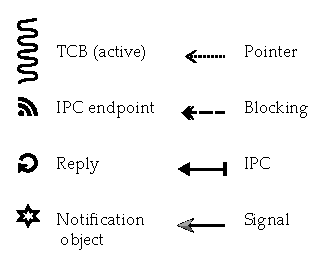
\includegraphics[width=0.5\textwidth]{legend-1}
    \caption{Legend for diagrams in this section}
    \label{f:legend-1}
\end{figure}

\subsection{Capabilities}
\label{s:capabilities}

As a capability-based \gls{OS}, access to any functionality in \selfour is via capabilities (recall
\Cref{s:os-capabilities}). Capabilities to all system resources are passed to the initial task --- the first
user-level thread started in the system --- which can then allocate resources as appropriate.
Capabilities exist in a \emph{capability space} that can be configured per thread or shared between
threads. 

Capability spaces are analogous to address spaces for virtual memory, and are formed of
\emph{CNodes} which contain capabilities. Where address spaces map virtual addresses to physical
addresses, capability spaces map object ids to access rights.  CNodes are analogous to page tables
in virtual memory, and can contain capabilities to further CNodes. A capability space address refers
to an individual entry in some CNode in the capability space, and may be empty or contain a
capability to a specific kernel resource. For brevity, a capability space address is referred to as
a slot. 

% access rights
Each capability has three potential access rights: read, right and grant. How those rights affect
the resource the capability provides access to depends on the type of resource, and is explained in
the next section.

% badges and operations
Various operations can be done on capabilities, which are summarised in \cref{t:capability_ops}.
When a capability is copied or minted, it is said to be \emph{derived} from the original capability.
All derived capabilities can be deleted by using \code{revoke}.
There are restrictions on which capabilities can be derived and under what conditions, depending on
what the capability provides access to. 
\emph{Badging} is a special type of derivation which allows specific capability types to be copied
with an unforgeable identifier. We discuss derivation restrictions and the use of badges further
in this chapter.
Any individual capability can be deleted, or revoked. The former simply removes a specific
capability from a capability space, the latter removes all child capabilities.

\begin{table}
    \centering
    \rowcolors{2}{gray!25}{}
    \begin{tabular}{l p{0.8\textwidth}}\toprule
    \emph{Operation}    & \emph{Description}\\\midrule
    \code{Copy}         & Create a new capability in a specified CNode slot, which is an exact copy
                         of the other capability and refers to the same resource. \\
    \code{Mint}         & Like copy, except the new capability may have diminished rights and/or be
                          badged. \\
    \code{Move}         & Move a capability from one slot to another slot, leaving the previous slot
                          empty. \\
    \code{Mutate}       & Like move, except the new capability may have diminished rights and/or be
                          badged. \\
    \code{Rotate}        & Atomically move two capabilities between three specified slots. \\
    \code{Delete}        & Remove a capability from a slot. \\
    \code{Revoke}        & Delete any capabilities derived from this capability. \\
    \code{SaveCaller}    & Saves the kernel generated resume capability into the designated slot. \\
    \bottomrule 
    \end{tabular}
    \caption{Summary of operations on capabilities provided by baseline \selfour~\citep{seL417}}.
     \label{t:capability_ops}
\end{table}


\subsection{Kernel Resources}

Capabilities provide access to specific objects, a brief summary of which is shown in
\cref{t:kernel_objects}. While the majority of objects in \selfour have a platform-dependant size fixed at compile time, some
are sized dynamically at runtime, \eg untyped and CNodes, which can be any power of two size.

% table of object types 
\begin{table}
    \centering
    \rowcolors{2}{gray!25}{}
    \begin{tabular}{l p{0.6\textwidth}}\toprule
    \emph{Object}    & \emph{Description}\\\midrule
    CNode            & A fixed size table of capabilities. \\
    \Gls{TCB}        & A thread of execution in \selfour.\\
    Endpoint  & Ports which facilitate \gls{IPC}. \\
    Notification object & Arrays of binary semaphores.\\
    Vspace     & Top level paging structure. \\
    PageTable  & Page table structures and address space IDs.\\
    Page       & Mappable physical memory. \\
    Interrupt & Allow access to specific hardware interrupts.\\
    Untyped    & Memory that can be retyped into other types of memory, including untyped.\\
    \bottomrule
    \end{tabular}
    \caption{Major object types in \selfour, excluding platform specific objects. For further detail
    consult the \selfour manual~\citep{seL417}}.
     \label{t:kernel_objects}
\end{table}



% control caps, normal caps
% operations

\subsection{Kernel memory management}

All kernel memory in \selfour is managed at user-level and accessed via capabilities
which is key to \selfour's isolation and security, but also essential for
understanding the complexity of kernel design.

Capabilities to objects can be copied, which creates another capability to the same object,
potentially with different access rights, but not
a copy of the object itself. 
Similarly capabilities to objects can also be deleted, but only when the last capability to an
object is deleted will the object itself be deleted. Object capabilities contain a pointer to the
actual kernel object. 

All memory in \selfour starts as \emph{untyped} memory, capabilities to which is granted to the
initial task in the system as part of the boot process. The initial task can then create all
types of memory, including further untyped, with an operation known as \emph{retyping}. As a result,
any object with a pointer to another object must have a back pointer to update should that object be
deleted, in order to avoid stray pointers in the kernel. 

\subsection{Untyped}


\subsection{Thread control blocks}

\Glspl{TCB} represent an execution context and manage processor time in \selfour. Each \gls{TCB} is
associated with a cspace and a top level virtual memory object, specified by capabilities, which may
be shared with other threads. 
Additionally threads have an IPC buffer, which is a page shared between the kernel and the thread
for messages. 
Threads have a timeslice attribute, which specifies the amount of milliseconds until that thread is
preempted, and a priority for the fixed priority scheduler.

% table of tcb invocations
\begin{table}
    \centering
    \rowcolors{2}{gray!25}{}
    \begin{tabular}{l p{0.8\textwidth}}\toprule
    \emph{Operation}    & \emph{Description}\\\midrule
        \code{Resume}               & Place a thread in the scheduler.\\ 
        \code{Suspend}              & Remove a thread from the scheduler.\\
        \code{WriteRegisters}       & Configure a threads execution context.\\
        \code{ReadRegisters}        & Read a threads execution context.\\
        \code{SetAffinity}          & Set the CPU on which this thread should run.\\
        \code{SetIPCBuffer}         & Set the page to use for the IPC buffer.\\
        \code{SetPriority}          & Set the priority of this TCB.\\
        \code{BindNotification}     & TODO \\
    \bottomrule 
    \end{tabular}
    \caption{Summary of operations on TCBs. Further operations are available that batch several
    setters to reduce thread configuration overheads.}.
     \label{t:tcb_ops}
\end{table}


\subsection{Endpoints}
\label{s:ipc}

\gls{IPC} is the microkernel mechanism for synchronous transmission of data and capabilities. In the \selfour model,
\gls{IPC} takes place via endpoints, which represent a general communication port. Any thread with a
capability to an endpoint can send and receive messages on that endpoint, subject to the access
rights. Most messages sent fit into registers, however messages exceeding this platform dependent
size are stored in the \gls{IPC} buffer, a kernel-writeable frame per
thread. 

IPC can be one-way, where the sender blocks until the message is sent then may continue
(\texttt{send()}) , or two-way,
where the sender blocks until a reply message is sent (\texttt{call()}). One-way IPC may also be
non-blocking, where the message is only sent if a receiver is already present.
Multiple senders and receivers can use the same endpoint, and which act as \gls{FIFO}
queues. 

\begin{figure}
    \centering
    \begin{subfigure}[h]{0.48\textwidth}
        \centering
        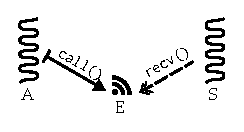
\includegraphics[width=\textwidth]{ipc1}
        \caption{Phase 1}
        \label{f:ipc1}
    \end{subfigure}%
    \begin{subfigure}[h]{0.48\textwidth}
        \centering
        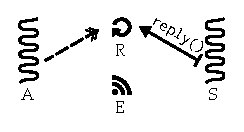
\includegraphics[width=\textwidth]{ipc2}
        \caption{Phase 2}
        \label{f:ipc2}
    \end{subfigure}
    \label{f:ipc}
    \caption{IPC phases: (a) shows the initial IPC rendezvous, (b) shows the
    reply phase. See \Cref{f:legend-1} for the legend.}
\end{figure}

Two-way IPC has two phases, as \cref{f:ipc} illustrates: rendezvous and reply.

\Cref{f:ipc1} demonstrates the rendezvous phase, where regardless of the order of operations, 
when one thread blocks (\cref{recv}) on the endpoint and another thread sends on that endpoint
then a message is sent. This occurs for both one-way and two-way \gls{IPC}.

The reply phase, illustrated in \Cref{f:ipc2}, only occurs if the sender used \texttt{call} to send
the \gls{IPC}. In this case, a one-off \emph{resume} capability is generated, which the caller ($A$)
blocks on, and the receiver ($S$) sends a reply message to, waking the caller. Receivers can save
the \emph{resume} capability to send a reply to later, but otherwise the resume capability is
installed in the \gls{TCB} CNode. The \emph{reply} system call directly invokes the resume
capability in this slot. 

% fastpath
Given \gls{IPC} performance is critical to overall system performance in a microkernel, \selfour
contains two \gls{IPC} fastpaths which is used when the following, common-case conditions are satisfied:

\begin{enumerate}
    \item the sender is using \texttt{call()} or the receiver is using \texttt{replyrecv()},
    \item there are no threads of higher priority than the thread being woken in the scheduler,
    \item the thread to be switch to has a valid address space and has not faulted,
    \item and the message fits in registers.
\end{enumerate}

Endpoint capabilities can be minted with unique, unforgeable badges which are delivered to the
receiver with the rest of the IPC message. This provides a mechanism for identifying senders.

\subsection{Fault handling}

\glspl{TCB} can have a specific fault endpoint registered, on which the kernel can send simulated
\gls{IPC} messages containing information about the fault. Fault handling threads can block on this 
endpoint. When a fault message is delivered to the fault endpoint, the kernel blocks the faulting
thread. The fault handling thread can then reply to this message to resume the thread and reset its
registers. If no fault endpoint is present, the
thread is rendered inactive and no fault message is sent. 

\subsection{Signalling}

Notification objects facilitate signalling in \selfour, either from other threads via \texttt{send()} or from
interrupts. The signals are non-blocking, as the badge of the notification capability is simply
bitwise ORed with a data word stored in the notification object itself. When a receiver blocks on a
notification object (\texttt{recv()}), if the badge has already been set it the receiver will
receive it immediately, otherwise the receiver will block immediately. Receivers can also poll a
notification object with \texttt{nbrecv()}.

% notifications, interrupts, aep-binding
\begin{figure}
    \centering
    \begin{subfigure}[h]{0.48\textwidth}
        \centering
        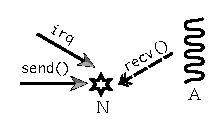
\includegraphics[width=\textwidth]{signal1}
        \caption{Notification}
        \label{f:signal1}
    \end{subfigure}%
    \begin{subfigure}[h]{0.48\textwidth}
        \centering
        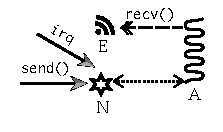
\includegraphics[width=\textwidth]{signal2}
        \caption{Bound notification}
        \label{f:signal2}
    \end{subfigure}
    \label{f:signal}
    \caption{Signals via a notification object. See \Cref{f:legend-1} for the legend.}
\end{figure}


\Cref{f:signal1} shows signal handling, where a thread A receives a signal and an interrupt at the
same time. In this case, the interrupt handler has a badged capability to the notification object,
$N$, as does the signaller. Both badges will be combined with a bitwise OR and delivered to the
receiver.

Signals can also be received by threads waiting on \gls{IPC}, as shown in \Cref{f:signal2}. A
\gls{TCB} object is bound to a notification object, establishing a link between them. Badges can be
used to determine whether a message was received from the endpoint or a signal on the notification object.

\subsection{System calls}

Over the last few sections we have indirectly presented several system calls for \gls{IPC} and
signalling. \Cref{t:system-calls} shows all the system calls available in \selfour. Communication
with the kernel itself is modelled as \gls{IPC} by using \texttt{call()} on kernel object
capabilities. Each capability has a set of \emph{invocations} which allow for methods on that object
to be used \eg binding a \gls{TCB} and notification object.

\begin{table} 
    \centering
    \rowcolors{2}{gray!25}{}
    \begin{tabular}{lp{0.6\textwidth}}\toprule
        \emph{System call} & \emph{Description} \\\midrule
        \texttt{send}      & One-way blocking \gls{IPC} or non-blocking signal.\\
        \texttt{nbsend}    & One-way non-blocking \gls{IPC} or non-blocking signal.\\
        \texttt{recv}      & Block waiting for a message or signal. \\
        \texttt{nbrecv}    & Poll for a message or signal. \\
        \texttt{call}      & Send an IPC and wait for a reply, or invoke the kernel. \\
        \texttt{reply}     & Send a message to the resume capability in the TCB CNode.\\
        \texttt{replyrecv} & \texttt{reply} and \texttt{recv} combined in one system call.\\
        \texttt{yield}     & Surrender current timeslice. \\
        \bottomrule
    \end{tabular}
    \caption{\selfour system call summary.}
    \label{t:system-calls}
\end{table}

\subsection{Thread states}

As depicted in \Cref{f:thread_state}, threads in \selfour can be inactive, running or blocked on a
specific object. The thread state encodes the object which the thread is blocked on. 

\begin{figure}[h!tb]
    \centering
    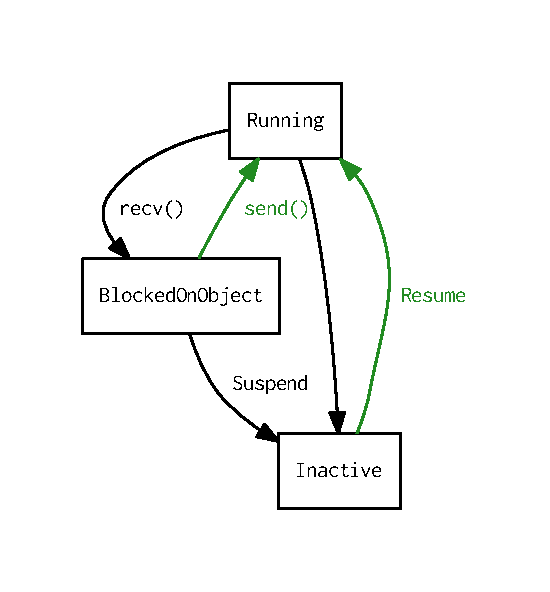
\includegraphics[width=1.1\textwidth]{thread_state}
    \caption{Thread state transitions in \selfour}
    \label{f:thread_state}
\end{figure}


\section{Scheduler}

The scheduler in \selfour is priority-based round-robin with 256 priorities (0 --- 255), implemented as an array of lists: one list of ready threads for each priority level. 
At a scheduling decision, the kernel chooses the head of the highest-priority, non-empty list, and
removes it from the relevant scheduler queue, which is referred to as \emph{Benno Scheduling}, named
after its original author.
The kernel previously used \emph{lazy scheduling}, leaving the current thread in its run queue, however this was replaced in favour of Benno scheduling to reduce the WCET of the kernel. 

Scheduling decision complexity is $O(1)$ as a two-level bit field tracks the highest priority with a runnable thread.

Kernel time is accounted for in ticks, with a static tick length defined at compile time (CONFIG\_TIMER\_TICK\_MS).
Threads have a timeslice field which represents the number of ticks they are eligible to run. 
This value is decremented every time a timer tick is handled, and when the timeslice is exhausted the thread is appended to the relevant scheduler queue, with a replenished timeslice.
The reload value of the timeslice is also defined at compile time (CONFIG\_TIME\_SLICE).

In an unrealistically simple system, where threads run at the same priority and do not communicate, it is possible to analyse temporal behavior on \selfour: threads will run for the timeslice value in round-robin order.
However, the allocation of ticks to threads is not actually that simple due to yield behaviour, preemption and \gls{IPC}. 

\subsection{Priorities}

Like any priority-based kernel without temporal isolation mechanisms, time is only guaranteed to the highest priority threads.
Priorities in \selfour act as informal capabilities: threads cannot create threads at priorities higher than their current priority, but can create threads at the same or lower priorities.
If threads at higher priority levels never block, lower priority threads in the system will not run.
As a result, a single thread running at the highest priority has access to 100\% of processing time.
However, even this becomes unclear once there is more than one thread at a priority: if two threads are running, they can both access 50\% of processing time.
If one of two threads blocks, the other gets 100\% of processing time and vice versa.
There is no way to enforce a certain processor allocation and how CPU time a thread receives is up
to priorities and the behaviour of other threads in the system, which is impossible to guarantee.

\subsection{Accounting}
% I think this should move to the design section?
\selfour has a tick-based scheduler, where ticks are accounted to the currently running thread,
meaning that temporal isolation in servers is not possible and accuracy is traded for precision, as
discussed in \Cref{s:tick-v-tickless}.

Similarly, the \texttt{yield} system call will not alter the timeslice of the current thread, and
only donates a portion of the current tick to the next thread in the round-robin scheduler. 

\subsection{Domain scheduler}

A recent addition to the \selfour kernel adds the ability to guarantee complete temporal isolation and deterministic scheduling between sets of threads, using the concept of scheduling \emph{domains}.
Threads are assigned to domains, each of which has a separate array of lists of threads over the priority range.
Each domain runs for a fixed amount of ticks, and domains are scheduled sequentially and deterministically.
Cross-domain \gls{IPC} is delayed until a domain switch, and \texttt{yield} between domains is not
possible. When there there are no threads to run while a domain is scheduled, a domain-specific idle thread will run until a switch occurs.

The domain scheduler can be leveraged to achieve temporal isolation however since domains cannot be
preempted, it is only useful for cyclic, non-preemptive scheduling with scheduling order and
parameters computed-offline.
In such a scenario each real-time task could be mapped to its own domain, and each task would run for its specified time before the domain scheduler switched to the next thread.
Any unused time in a domain would be wasted, and spent in the idle thread.

Such a scheduler is only suitable for closed systems and results in low system utilisation.
Dynamic real-time applications with shared resources and high system utilisation are not compatible
with the domain scheduler, as they require preemption.

\section{RT support}

We introduced basic \selfour concepts and terminology, and investigated mechanisms that effect
timing behaviour in the kernel: the scheduler, priorities, yield and IPC. 
In this section we will look at how real-time scheduling could be implemented with those mechanisms.

There are several options for implementing a real-time scheduler in the current version of \selfour: leveraging the domain scheduler, using the priority scheduler or implementing a scheduling component to run at user-level. 
The domain scheduler offers low utilisation for strictly closed
systems with strict temporal partitioning and no preemption, so is clearly insufficient, as
discussed in \Cref{sec:rt-scheduling}.

The priority scheduler could be leveraged to implement a rate-monotonic scheduler.
However, this requires complete trust in every thread in the system, as there is no mechanism for temporal isolation: if one thread executes for too long, other threads will miss their deadlines.
Essentially the only thread with a guaranteed CPU allocation is the highest priority thread, which under rate-monotonic priority assignment is not the most critical thread in the system, but the thread with the highest rate.
Additionally, periodic threads driven by timer interrupts rather than events would need to share a user-level timer.

\begin{table}
	\centering
	\begin{tabular}{lp{2cm}p{2cm}p{2cm}p{2cm}} \toprule
        & \emph{Temporal isolation} & \emph{Utilisation} & \emph{Low kernel overheads} &
        \emph{Dynamic}\\
        \midrule
Domain scheduler          & \yes               & \no         & \yes        & \no    \\
Priority scheduler        & \no                & \yes        & \yes        & \yes   \\
Trusted timer component   & \yes               & \yes        & \no         & \yes   \\
        \bottomrule
	\end{tabular}
	 \caption{Comparison of existing \selfour scheduling options -- nothing ticks all of the boxes.}
	 \label{tab:nothing-ticks-all-boxes}
\end{table}


To build a dynamic system with temporal isolation and high CPU utilisation, one could implement a trusted timer component at user-level.
This component would be the highest priority thread in the system, and could pause threads to prevent them from overrunning their assigned rate.
However, since the timer component would need to maintain accounting information and track the currently running thread, it would need to be invoked for every single scheduling operation.
This is prohibitively expensive, as it results in doubled context switching time and increased number of system calls for thread management.

\Cref{tab:nothing-ticks-all-boxes} shows a comparison of all of the available scheduling options in the current version of \selfour -- no option provides all of the qualities we require.
Clearly, the kernel needs something more. 
In the next section we will our model for a more principled approach to time by extending the
baseline \selfour model presented in this chapter. We incorporate using the principles of resource kernels and with the aim of support diverse task sets, including those for mixed-criticality systems.


\chapter{Design \& Model}
\label{chap:model}

We now present our design and model for mixed-criticality scheduling support in a high-assurance
system such as \selfour. 

Our goal is to provide support in the kernel for mixed-criticality workloads.  This involves
supporting tasks of different time sensitivity, (\gls{HRT}, \gls{SRT}, best-effort), different
criticalities, and different levels of trust.  Such tasks should not be forced into total
isolation, but be permitted to share resources without violating their temporal correctness
properties through mechanisms provided by the kernel.

To achieve this we require temporal isolation: a feature of resource kernels, whose mechanisms we
apply to our research platform, \selfour.  However temporal isolation is not enough: mixed-criticality
systems require asymmetric protection rather than temporal isolation, as a result we leverage
traditional resource kernel reservations but decouple them from priority, allowing the processor to
be overcommitted while providing guarantees for the highest priority tasks.

In this section we first address how we integrate resource kernel mechanisms with \selfour with
mechanisms for temporal isolation. We then describe our mechanisms for temporal isolation of
resources shared between clients of different levels of criticality, time sensitivity, and trust.
Finally, we show how our mechanisms can be used to build several existing user-level policies. 

Our design goals are as follows:
\begin{description}\sloppy
    \item[Capability-controlled enforcement of time limits:] In general, capabilities
      help to reason about access rights. Furthermore, they allow a
        seamless integration with the existing capability-based spatial
          access control of security-oriented systems such as \selfour.
    \item[Policy freedom:] In line with microkernel philosophy
        \citep{Heiser_Elphinstone_16}, the model should not force systems
        into a particular resource-management policy. In particular, it
        should support a wide range of scheduling policies and
        resource-sharing models, such as locking protocols.
    \item[Efficient:] The model should add minimal overhead over the best
                      existing implementations. In particular, it should be compatible
                        with fast \gls{IPC} implementations in high-performance microkernels.

    \item[Temporal isolation:] The model must allow system designers to create systems where a
        temporal failure in one component cannot cause a temporal failure in another part of the
        system.

    \item[Overcommitment:] The model must allow systems to be specified that are not necessarily
        schedulable: as the degree and nature of overcommitment is a core policy of a particular
        system. Overcommitment is also key to providing  asymmetric protection, where high
        criticality tasks can disrupt low criticality tasks.

    \item[Safe resource sharing:] Temporal isolation should persist even in the case of
        shared-resources, to provide mechanisms for sharing between applications with different
        levels of time-sensitivity, criticality and trust.
\end{description}

The model  provides temporal isolation mechanisms from the kernel, while allowing for more complex
scheduling policies to be implemented at user level.

\section{Scheduling}

We outlined four core resource kernel mechanisms---admission, scheduling, enforcement and
accounting---that are essential to resource kernels for implementing temporal isolation.  However,
as noted in \Cref{sec:resource-kernels}, such kernels are monolithic, where all policy, drivers and
mechanisms are provided by the kernel.

Microkernels like \selfour offer a different design philosophy, based on the principle of
minimality~\citep{Liedtke_95}, where mechanisms are only included in the kernel if they would
otherwise prevent the implementation of required functionality. Previous resource kernels
are all monolithic, where all resource policies are implemented in the kernel itself.

The goals of resource kernels do not directly align with that of microkernels in general.  This is
because microkernels do not directly manage all resources in the system, but provide mechanisms for
the system designer to implement custom resource management policies.  

In \selfour, mechanisms for physical memory, device memory, interrupt and \IO port management are
exposed to the user via the capability system, as outlined in \cref{chap:sel4}. As a result, the
only resource that the kernel needs to provide reservations for is processing time.  We now present
our mechanisms, and discuss how each of the four resource kernel policies can be implemented within our model.

\subsection{Scheduling}
\label{sec:model-scheduling}

There are two design choices relevant to scheduling:

\begin{itemize} 
    \item Should a scheduler be provided in the kernel at all? 
    \item Should the scheduling algorithm be fixed (\gls{FP}) or dynamic (\gls{EDF}) priority?
\end{itemize}

\subsubsection{Kernel scheduling}

We retain the scheduler in the kernel, unlike \composite, for two reasons: to
maintain a small trusted computing base, and for performance. Any system with
multiple threads of execution, which is required in a mixed-criticality system,
must have a scheduler, which for the purposes of temporal isolation is part of
the trusted computing base. If a system must have a scheduler, and in a
mixed-criticality system, with untrusted components, that scheduler must be in
a separate protection domain to those untrusted components, then a scheduling
decision will require at least two context switches: from the preempted thread
to the scheduler, and from the scheduler to the chosen thread. Placing a basic
scheduler in the kernel reduces this overhead. 

Additionally, as the scheduler is a core component of the system it must be
verified: by keeping the
scheduler in the kernel we maintain the current verification. Verification of a user-level scheduler
and its interaction with the kernel is a far more complex task, especially as verification of
concurrent systems is very much an open research challenge. 

One might claim maintaining a scheduler in the kernel is a violation of our goal of policy freedom.
However, we maintain this is not the case, which comes down to our choice of fixed priorities over
\gls{EDF}.

\subsubsection{Fixed priorities}

Our model uses \gls{FP} scheduling as a core part of the kernel, with the addition of mechanisms
that allow for the efficient implementation of user-level schedulers.
We choose \gls{FP} over \gls{EDF} for three reasons; 
fixed-priority is dominant in industry
as shown in \cref{chap:operating-systems} and maps well to \gls{FP} with \gls{RM} priority assignment; and dynamic scheduling policies like
\gls{EDF} can be implemented at user level; and \gls{FP} has defined behaviour on overcommitted
systems.

\gls{EDF} scheduling can be implemented by using a single priority for the dynamic
priorities of \gls{EDF}, as we will demonstrate in \cref{s:edf-impl}.
However, the opposite is not true: mapping the dynamic priorities of EDF to a fixed-priority
is non-trivial and would come with high overheads. 
Our approach is consistent with existing designs in Linux  and ADA~\citep{Burns_Wellings:crtpa}, which
support both scheduling algorithms, usually with \gls{EDF} at a specific priority. Additionally,
schedulability analysis of \gls{EDF}-within-priorities is well
understood~\citep{Harbour_Palencia_03}.

We do not consider Pfair scheduling (recall \cref{s:pfair}) an option, as its high interrupt
overheads and fairness properties are not suitable for hard real-time systems.  Again however, it is
possible to implement a Pfair scheduler at user level.

The final reason to base the approach on fixed priorities is the ability
to reason about the behaviour of an
overcommitted system. Overcommitting, is important for achieving high
actual system utilisation, given the large time buffers required by
critical hard real-time threads. It is also essential to keeping the kernel
policy-free: The degree and nature of overcommitment is a core policy
of a particular system. For example, the policy might require that the
total utilisation of all \crit{high} threads is below the \gls{FPRM}
schedulability limit of 69\%, while \crit{low} threads can overcommit,
and the degree of overcommitment may depend on the mix of hard RT,
soft RT and best-effort threads. Such policy should be defined and
implemented at user level rather than in the kernel.

As discussed in \autoref{s:overload}, the result of overload in an
EDF-based system is hard to predict, and such a system is hard to
analyse. In contrast, with fixed priority the result is easy to
understand: If the sum of utilisations of threads at priority \(\geq
P\) is below the utilisation bound, then all those threads will meet
their deadlines, while any thread with priority \(<P\) may miss. This
allows easy analysis of schedulability.

\subsection{Scheduling contexts}
\label{sec:model-scheduling-contexts}

At the core of the model is the \emph{\gls{SC}} as the
fundamental abstraction for time allocation, and the basis of 
the enforcement and accounting mechanisms in our model.
An \gls{SC} is a representation
of a reservation in the object-capability system, which means that 
they are first-class objects, like threads, address spaces, or
\gls{IPC} endpoints. An SC is represented by a capability to a
scheduling context object.

In order to run, a thread needs an \gls{SC}, which represents the
maximum CPU bandwidth the thread can consume. Threads obtain \glspl{SC} through \emph{binding}, and
only one thread can be bound to an \gls{SC} at a time to avoid hierarchical scheduling.
In a multicore system, an SC represents the right to access a
particular core. Core migration, \eg for load balancing, is policy
that should not be imposed by the kernel but implemented at user
level. A thread is migrated by replacing its SC with one tied to a
different core. This renders the kernel scheduler a partitioned scheduler, 
which aligns with our efficiency goal; partitioned schedulers outperform global
schedulers~\citep{Brandenburg:phd}.

The unfungible nature of time in real-time systems requires that the
bandwidth limit must be enforced within a certain time window. We
achieve this by representing an SC by sporadic task parameters, \emph{period}, \(T\), and a
\emph{budget}, \(C\), where \(C\leq T\) is the maximum amount of time
the SC allows to be consumed in the period. \(U=\frac{C}{T}\) represents the
maximum \emph{CPU utilisation} the SC allows. The SC can be viewed as
a generalisation of the concept of a time slice, discussed in \cref{s:timeslices-and-meters}.

In order to support MCS, we do not
change the meaning of priority, but what it means for a thread to be
\emph{runnable}: We associate each thread with an SC, and
make it non-runnable if it has exhausted its budget. 


\glspl{SC} can be gracefully integrated into the 
existing model used in \selfour,
logically replacing the time slice attribute with the scheduling context object.

Unlike \fiascooc's scheduling contexts~\citep{Lackorzynski_WVH_12}, which
are superficially similar to ours, we retain priorities as a thread
attribute rather than making them part of \glspl{SC}\footnote{\fiascooc's scheduling
contexts are not integrated in to the capability system.}. The advantage of keeping the two
orthogonal will become evident in \cref{s:locking}.

\subsection{Accounting}
\label{sec:model-accounting}

Accounting must be a mechanism implemented by the kernel, as the kernel is the only entity in the system
that can monitor all threads, regardless of preemption in the system, since the kernel facilitates all
preemption.
The accounting mechanism is provided by new system invariant that the currently running thread 
must have a scheduling context with available budget, as all time consumed is billed to the
current scheduling context.
This includes time spent executing in the kernel, including preemptions.
The rule for accounting kernel time is all time, from kernel entry, is billed to the scheduling
context active on kernel exit. This means that if a thread is preempted and 
that preemption does not trigger a switch to a 
different scheduling context, all time is accounted to the current scheduling context. Otherwise, 
time from kernel entry is accounted to the next scheduling context.

In order to facilitate user-level schedulers, the kernel tracks the amount of time consumed by a
scheduling context, which can be retrieved by an invocation on that specific scheduling context
object.
We specifically do not cater for dynamic frequency scaling and ensure that it is turned off
during testing---this is out of scope and a topic for future work. 

\subsection{Admission control}
\label{sec:model-admission}

Unlike any previous kernel that supports reservations, our model delegates admission control to user
level, as it is deeply tied to policy, which a microkernel should not limit. A consequence of this
choice is the design naturally supports over-commitment, as this is part of the admission test.

The mechanisms for admission control consist of two parts: scheduling contexts are created without
any budget at all, and a new control capability must be invoked to populate scheduling context
parameters.
\schedcontrol is the new control capability, one of which is provided per processing core,
and grants authority to 100\% of time on that core, thus providing the admission-control privilege.
This is analogous to how \selfour controls the right
to receive interrupts, which is controlled by the IRQ\_control
capability as introduced in \cref{s:control-capabilities}. Like time, IRQ sources are non-fungible.

Unlike the reservations in resource kernels, the scheduling context does not 
act as a lower-bound on CPU bandwidth that a thread can consume. This, combined with
user-level admission control, is also key to allowing system designers to over-commit the system. 

By designating admission tests as user-level policy, we allow system designers complete freedom
in determining which admission test to use, if at all, and when that test should be done.
Consequently, they can be run dynamically at run-time, or offline, as per user-level policy.

Thus, the kernel places no restriction on the creation of reservations apart from minor integrity
checks (\ie $C \leq T$).
For example, some high-assurance systems may sacrifice utilisation for safety with a very basic but easily verifiable, online, admission test.
Other implementations may conduct complex admission tests offline in order to obtain the highest possible utilisation, using algorithms that are not feasible at run time.
Some systems may require dynamic admission tests that sacrifice utilisation or have increased risk.
Basic systems may require a simple break up of the processing time into rate-limited reservations.
By taking the admission test out of the kernel, all of these extremes (and hybrids of) are optional policy for the user.

A consequence of this design is that more reservations can be made than processing time available.
This is a desirable feature: it allows system designers to overcommit the system, while features of the scheduling mechanisms provided by the kernel guarantee that the most important tasks get their allocations, if the priorities of the system are set correctly.

However, allowing any thread in the system to create reservations could result in overload behaviour and violation of temporal isolation.
To prevent this, admission control is currently restricted to the task that holds the scheduling
control capability for each processing core.

\subsection{Replenishment}

Scheduling contexts can be \emph{full} or \emph{partial}. A thread with a \emph{full} SC, where
\(C=T\), may monopolise whatever
CPU bandwidth is left over from higher-priority threads, while high-priority threads with full
\glspl{SC} may monopolise the entire system. 
Partial \glspl{SC}, where \(C<T\), are not runnable once
they have used up their budget, until it is replenished, and form our mechanism for temporal
isolation.  

Full \glspl{SC} are key to maintaining policy freedom and performance; while systems
must be able to use our mechanisms to enforce upper bounds on execution, the usage of 
those mechanisms is policy. If a task is truly trusted, no enforcement is required,
as in standard \gls{HRT} systems. They can also be used for best-effort threads which run in slack time.
The \(C\) of a full \gls{SC} represents the timeslice, which once expired results in round robin
scheduling at that priority. Additionally, full \glspl{SC} provide legacy compatibility: setting \(C\ = T =\)
the previous timeslice value results in the same behaviour as the master kernel. 

From a performance perspective full \glspl{SC} prevent mandatory preemption overheads 
that derive from forcing all threads in a system to have a reservation. Threads with a full
budget incur no inherent overhead other than the preemption rate $1/T$.

Threads with \emph{partial} \glspl{SC} have a limited budget, which forms an upper
bound on their execution. For replenishment, we
use the sporadic servers model as described in \cref{p:sporadic} with an
implementation based on the algorithms presented
by~\citet{Stanovic_BWH_10}. 

The combination of full and partial \glspl{SC}  and the ability to overcommit distinguishes our
model from that of resource kernels.

\subsubsection{Sporadic servers}
\label{sec:model-sporadic}

We use sporadic servers as they provide a mechanism for isolation without requiring the kernel
to have access to all threads in the system, unlike other approaches discussed in
\cref{background:fp-isolation}, \eg  priority exchange servers and slack stealing.
Deferrable servers do not require global state but are avoided due to the back-to-back
problem.
Avoiding global, shared-state is required for confidentiality, because access to shared state
has cache effects, which leak information via cache-based timing-channels. In order to maintain these properties,
timing channels must be mitigated through partitions. 
It must be possible to partition a system completely, such that operations in one partition do not
alter the cache state in the other partitions.

Recall that sporadic servers work by preserving the
\emph{sliding window} constraint, meaning that during any time
interval not exceeding the period, no more than $C$ can be consumed.
This stops a thread from saving budget until near the end of its
period, and then running uninterrupted for more than $C$. It is achieved by tracking any leftover
budget when
a thread is preempted at time \(t\), and scheduling a replenishment for time  $t+T$.

In practice, we cannot track an infinite number of
replenishments, so in a real implementation, once the number of
queued replenishments exceeds a threshold, any excess budget is
discarded. If the threshold is one, the behaviour degrades to polling
servers~\citep{Sprunt_SL_89a} where any unused budget is lost and the
thread cannot run until the start of the next period. 

There is an obvious cost to replenishment fragmentation that will
arise from preemptions, and polling servers are more efficient in the
case of frequent preemption \citep{Li_WCM_14}; an arbitrarily high
threshold makes little sense. The optimal value depends on
implementation details of the system, as well as the characteristics
of the underlying hardware.

We therefore make the threshold an attribute of the SC. \glspl{SC} are variably sized,
such that system designers can set this bound per SC. This is a generalisation of the approach used
in Quest-V~\citep{Danish_LW_11}, where \IO reservations are polling servers and other reservations 
are sporadic servers, as policy which can easily be implemented at user-level with variably sized
\glspl{SC}.

\subsection{Enforcement}
\label{sec:model-enforcement}

Threads may exhaust their budgets for different reasons. A budget may
be used to rate-limit a best-effort thread, in which case budget
overrun is not different to normal time-slice preemption of
best-effort systems. A budget can be used to force an untrusted thread
to adhere to its declared WCET. Such an overrun is a contract violation, which may be reason
to suspend the thread or restart its subsystem. Finally, an overrun by
a critical thread can indicate an emergency situation; for example,
critical threads may be scheduled with an optimistic budget to provide
better service to less critical threads, and overrun may require
provision of an emergency budget or specific exception handler.

Clearly, the handling of overrun is a system-specific policy, and the
kernel should only provide appropriate
mechanisms for implementing the desired policy. Our core mechanism is
the \emph{timeout exception}, which is raised when a thread is
preempted due to budget expiry. To allow the system to handle the exceptions, each thread
is optionally associated with a timeout exception handler, which is
the temporal equivalent to a (spatial) protection exception. When a
thread is preempted, the kernel notifies its handler via an \gls{IPC} message. The
exception is ignored when the thread has no timeout exception handler, and the thread
can continue to run once its budget is replenished.

The timeout fault
endpoint is separate from the existing thread fault endpoint, as the semantics are different,
because non-timeout faults are not recoverable without the action of another thread. 
While threads are not required to have a fault endpoint, when a fault occurs a thread is always
blocked, as it is no longer in a runnable state. Timeout faults on the other hand are recoverable:
the thread must simply wait until budget replenishment. 

Timeout fault handling threads should have their own \gls{SC} to run on, with enough budget to handle
the fault, otherwise they will not be eligible for selection by the kernel scheduler.

Similar to a page fault handler, timeout fault handlers can be used to adjust thread parameters
dynamically as may be required for an \gls{SRT} system, or raise an error.
The handler has a choice of a range of overrun policies, including:
\begin{itemize}
      \item providing a one-off (emergency) budget to the thread and letting it continue,
       \item permanently increasing the budget in the thread's SC, and
       \item killing/suspending the thread.
       \end{itemize}
Obviously, these are all subject to the handler having sufficient
authority (\eg \schedcontrol).

If a replenishment is ready at the time the budget expires, the thread
is immediately runnable. It is inserted at the end of the ready queue
for its priority, meaning that within a priority, scheduling of
runnable threads is round-robin.

The timeout fault handler is similar to the original KeyKOS~\citep{Bomberger_FFHLS_92} concept of
meters, which was carried through to earlier L4 microkernels as a \emph{preempter}. The preempter was
invoked every time the timeslice/meter expired to make a scheduling decision. This was abandoned due
to performance reasons. Our approach differs in that timeout fault handlers are optional, so that
they can be used in exceptional scenarios only. However, timeout fault handlers can also be used to
facilitate user-level scheduling, which is now feasible as modern hardware has much faster context
switch times. 

\subsection{Priority assignment}

Assignment of priorities to threads is user-level policy. One approach is to simply use
rate-monotonic scheduling: where priorities are assigned to threads based on their period, and
threads use scheduling contexts that match their sporadic task parameters.  Each thread in the
system will be temporally isolated as the kernel will not permit it to exceed the processing time
reservation that the scheduling context represents.

However, the system we have designed offers far more options than simple rate-monotonic fixed-priority
scheduling.  Policy freedom is retained as reservations simply grant a potential right to processing
time, at a particular priority.  What reservations actually represent is an upper bound on
processing time for a particular thread.  Low priority threads are \emph{not} guaranteed to run if
reservations at higher priorities use all available CPU.  However, threads with reservations at low
priorities will run in the system slack time, which occurs when threads do not use their entire
reservation.

The implication is that a system could use a high range of priorities for rate-monotonic threads,
while best-effort and rate-limited threads run at lower priorities.  Another alternative is to map
user-lever schedulers to specific  priorities, for instance an EDF scheduler. 

\subsection{Asymmetric Protection}

Recall that in a mixed-criticality system, asymmetric protection means that tasks with higher
criticality can cause deadline misses in lower criticality tasks.  Two approaches to mixed
criticality scheduling that provide asymmetric protection are slack scheduling and
\gls{RTA}~\citep{Burns_Davis_17}.

Under slack scheduling, low-criticality tasks run in slack time of high-criticality tasks.  Our
model supports this easily: high-criticality tasks are given reservations to all processing time at
high priorities, and low-criticality tasks are given reservations at a lower priority band.

\gls{RTA} relies on suspending or de-prioritising low-criticality tasks if a high-criticality
task runs for longer than expected.  Simple \gls{RTA} schemes involve two system modes:
a \crit{HI} mode and a \crit{LO} mode, although they have been generalised to
more~\citep{Fleming_Burns_13}.  In \crit{LO} mode, high-criticality tasks run with smaller 
reservations, and the remaining
CPU time is used for low-criticality tasks.  If a high-criticality task does not complete before its
\crit{LO}-mode reservation is exhausted, the system switches to \crit{HI} mode: all low criticality
tasks are suspended.  Such a criticality switch is also supported by our model, at user-level: a high-priority scheduling thread can be
set up to receive temporal faults when a task does not complete before its budget expires.  On a
temporal fault, the scheduling thread can modify the scheduling parameters of tasks appropriately,
for example by boosting the high-criticality task's priority and budget.

\subsection{Summary}

The scheduling, accounting and enforcement mechanisms presented are sufficient to support temporally
isolated, fixed-priority or \gls{EDF} scheduled real-time threads. By keeping admission control
out of the kernel we preserve policy freedom, while the mechanisms provided allow for a full
resource kernel to be built, or other types of system which require the ability to over-commit.
Additionally, we have maintained
support for best-effort threads, and have added the ability to provide asymmetric protection for
mixed-criticality workloads. 
In the next section, we show how our model provides mechanisms for resource sharing. 

\section{Resource sharing}\label{s:locking}

Reservations through the mechanism of scheduling contexts are not sufficient alone to provide
resource sharing between tasks of different time-sensitivity, criticality, and trust. We now
present how the scheduling context mechanism facilitates resource sharing policies 
in terms of the three core mechanisms ---prioritisation, charging and enforcement---presented 
in \cref{sec:resource-kernels}.

In this section we consider only resources shared by resource servers in a \gls{RPC} style where
servers are scheduled directly as a result of the \gls{RPC}. Other forms of resource sharing, such
as the asynchronous multicast provided by ARINC 653 (\cref{s:arinc}), are possible, but not
relevant, as time is not directly exchanged, and we have already shown how temporal partitioning is possible with
reservations. 

RPC-style shared servers are fundamentally a trusted entity: the client does not resume until the
server replies to a request, and the server may not ever reply. Additionally, the client requires the
server to carry out the operation requested. Consequently, the server takes on the ceiling of the
requirements of all the clients. If a server is shared between trusted and untrusted clients, the
server must be trusted as much as the most trusted client. If a server is shared between \gls{HRT}
and best-effort clients, the server must have the same time sensitivity as the HRT clients: a defined 
\gls{WCET} and bounded blocking behaviour. Finally, the server must be at the highest criticality
level of all clients, however the opposite is not true. If a server has sufficient isolation
properties, then all the clients of that server are not also promoted to the
highest criticality level, which as we know greatly increases the certification burden. 

This asymmetry also holds for trust: a trusted server need not trust its clients,
and the clients need not trust each other. 
Trusted scenarios do not require this level of encapsulation: user-level threads packages can implement
locking protocols with libraries such as \texttt{pthreads}. Therefore, our focus is on temporal
isolation in shared servers beyond strict partitioning, where clients do not trust each other, and
the server does not trust the client.

The proposed model supports shared servers, including scheduler
bypass, through \emph{scheduling context
donation}: a client invoking a server can pass its SC along, so the
server executes on the client's SC, until it replies to the
request. This ensures that the time consumed by the server is billed
to the client on whose behalf the server's work is done. If the scheduling context 
expires, the enforcement mechanism of timeout exceptions can be used to recover the server according 
to server specific policy.

\subsection{Prioritisation}

We indicated in \Cref{sec:model-scheduling-contexts} that scheduling contexts are separate from thread control blocks in
order to support resource sharing. Additionally, unlike previous microkernel designs for \glspl{SC}, priority
remains an attribute of the execution context. Decoupling priority and scheduling context avoids
prior patterns where priority-inheritance is enforced by the kernel. 

The \Gls{IPCP} maps neatly to this model: if server threads are assigned the ceiling protocol of all of
their clients, then when the \gls{IPC} rendezvous occurs and we switch from client to server, the
server's priority is used, a consequence of decoupling priority from the scheduling context.
\gls{IPCP} is also practical: it is mandated by the AUTOSAR standard
(recall \cref{sec:os-autosar}) and is therefore understood well by parts of the industry.

The main drawback of the \gls{IPCP}, namely the requirement that all
lockers' priorities are known \emph{a priori}, is easy to enforce in a
capability-based system: The server can only be accessed through an
appropriate invocation capability, and it is up to the system designer
to ensure that such a capability can only go to a thread whose
priority is known or appropriately controlled.

The choice of the \gls{IPCP} over other fixed-priority protocols, the \gls{PIP} and the \gls{OPCP},
is intentional, and we now present the case against both protocols.

In order to properly support real-time systems, our model orders endpoint queues by priority, rather
than the traditional \gls{FIFO} of L4 kernels. Threads of the same priority remain FIFO. 

\subsubsection{\gls{PIP}}

The major factor in ruling the \gls{PIP} out as a mechanism provided by the microkernel is
performance. Introducing \gls{PIP} would drastically increase scheduler operations on the critical
\gls{IPC} fastpath, as priorities would need to be returned on the reply path. One could take after
Real-time Mach, and provide \gls{PIP} as an optional flag on a message port, thereby retaining
policy freedom, but at a performance cost. Mandating the \gls{PIP}, which incurs a high-preemption
overhead compared to other protocols, would violate both our performance and policy freedom
requirements. 

There is an additional, practical concern, in that the \gls{PIP} does not map well to the existing
capability system. Recall from \cref{p:sel4_ipc} that endpoints have very minimal state\footnote{Which
again contributes to high performance.}, and once an \gls{IPC} rendezvous has occurred, the caller is
blocked on the resume capability. Consequently, there is \emph{no way to reach the caller} after an 
\gls{IPC} message has been sent. 
Significant changes would be required to the \gls{IPC} model to ensure threads
blocked on resume capabilities could be tracked from the endpoint that the message was sent over.



\subsection{\gls{OPCP}}

Although the \gls{OPCP} offers greater processor utilisation than the \gls{IPCP}, it would require the
kernel to track a system ceiling and also implement priority inheritance, in a form where unrelated
threads may inherit priorities due to a resource access pattern. Both of these mechanisms are
required to implement the \gls{OPCP}, and both would violate confidentiality by altering state 
across partitioned resources.  This is the same reason we exclude
priority-exchange and slack-stealing servers, as discussed in \cref{sec:model-sporadic}.

Although not provided by the kernel, \gls{PIP} and \gls{OPCP} can be implemented at user-level if
required, by proxying requests to shared resources via an endpoint and thread which manipulates the priorities
appropriately, before forwarding on the request. For \gls{PIP}, only one extra thread per resource would 
be required and could exist in the same address space as the resource.
Since \gls{OPCP} requires global state, an implementation would require a shared service for all threads 
sharing a set of resources. We describe such an implementation in \cref{sec:model-mechanisms} after introducing further mechanisms
in \cref{sec:model-policies}.

\subsection{Charging}

\begin{figure}
    \centering
    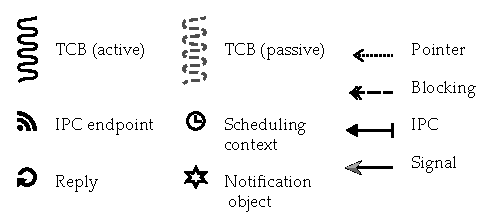
\includegraphics[width=0.7\textwidth]{legend-full}
    \caption[Legend for diagrams in this chapter.]{Legend for diagrams in this chapter, an expanded version of \cref{f:legend-1}}
    \label{f:legend-2}
\end{figure}


\begin{figure}
    \centering
    \begin{subfigure}[h]{0.48\textwidth}
        \centering
        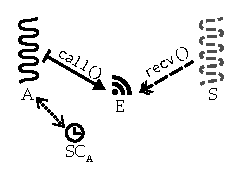
\includegraphics[width=\textwidth]{passive1}
        \caption{Phase 1}
        \label{f:passive1}
    \end{subfigure}%
    \begin{subfigure}[h]{0.48\textwidth}
        \centering
        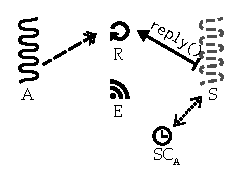
\includegraphics[width=\textwidth]{passive2}
        \caption{Phase 2}
        \label{f:passive2}
    \end{subfigure}
    \caption[IPC phases between an active client and passive server.]{IPC phases between an active client and passive server: (a) shows the initial \gls{IPC} rendezvous, (b) shows the
    reply phase. The client's $SC_{A}$ is donated between client and server. See \Cref{f:legend-2} for the legend.}
    \label{f:passive}
\end{figure}
\begin{figure}
\centering
\begin{subfigure}[h]{0.48\textwidth}
    \centering
    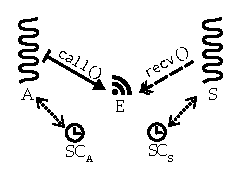
\includegraphics[width=\textwidth]{active1}
    \caption{Phase 1}
    \label{f:active1}
\end{subfigure}%
\begin{subfigure}[h]{0.48\textwidth}
    \centering
    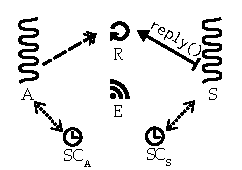
\includegraphics[width=\textwidth]{active2}
    \caption{Phase 2}
    \label{f:active2}
\end{subfigure}
\caption[IPC phases between active client and active server.]{IPC phases between an active client and active server: (a) shows the initial \gls{IPC} rendezvous, (b) shows the
reply phase. Both client and server have their own SC. See \Cref{f:legend-2} for the legend.}
\label{f:active}
\end{figure}

Charging for time executed in a server is simple in our model: charge the scheduling
context that the resource server is running on.
The question is, \emph{which} scheduling context is the server running on? Unlike
previous implementations of donation like semantics, our model does not mandate
scheduling context donation. Resource servers are free to run on their own scheduling context, 
according to the policy of the system.

Whether donation occurs or not is inferred at the time of the \gls{IPC} rendezvous: we test if the
server is passive or active. 
\emph{Passive} servers do not have a scheduling context 
and receive them over \gls{IPC} whereas \emph{active} servers have their own scheduling context. 
Passive servers, as illustrated in \cref{f:passive}, effectively provide a migrating-thread
model~\citep{Ford_Lepreau_94, Gabber_SBBS_99}, but without requiring
the kernel to manage stacks. \Cref{f:active} shows active servers, which allow system designers to
build systems without temporal isolation, as it is not suitable
for all systems.

\subsection{Enforcement}

If a passive resource server exhausts the scheduling context it is running on, it and any waiting clients
are blocked until replenishment. On its own, this means that a client
not only has to trust its server, but all the server's other
clients. This would rule out sharing a server between clients of
different criticality.

In a \gls{HRT} system, we can assume that a client's reservations are sufficient to complete
requests to servers.  However, in systems with best-effort and soft real-time tasks, no such
assumption can be made and client budgets may expire during a server request.  This leaves the
server in a state where it cannot take new requests as it is stuck without an active reservation to
complete the previous request.  Without a mechanism to handle this event the server, and any
potential clients, would be blocked until the client's budget is replenished.

Timeout exceptions can be used to remove this need for trust, and
allow a server to be shared across criticalities, as depicted in \cref{f:timeout}. Timeout fault endpoints are specific to the
execution context of a thread, not the scheduling context. Consequently, servers may have timeout
fault handlers while clients do not. The 
server's timeout handler can, for example, provide an emergency budget
to continue the operation (useful for \crit{HI} clients) or abort
the operation and reset or roll back the server. The latter option is
attractive for minimising the amount of budget that must be reserved
for such cases.

\begin{figure}
    \centering
    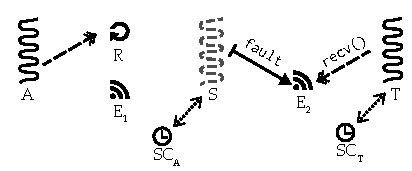
\includegraphics[width=0.8\textwidth]{timeout}
    \caption[Example of a timeout exception handler.]{Example of a timeout exception handler. The passive server $S$ performs a request on
    client $A$'s scheduling context, $SC_{A}$. A timeout fault is generated when $SC_{A}$ is
exhausted and sent to the server's timeout fault endpoint $E_{2}$, and the timeout handler receives
it. See legend \cref{f:legend-2}}
    \label{f:timeout}
\end{figure}


A server running out of budget constitutes a protocol violation
by the client, and it makes sense to penalise that
client by aborting. Helping schemes, such as \gls{PIP} or bandwidth
inheritance,
make the waiting client pay for
another client's contract violation. This not only weakens temporal isolation,
it also implies that the size of the required reserve budget
must be a server's full WCET. This places a restriction on the server
that no client request exceed a blocking time that can be tolerated by
all clients, or that all clients must budget for the full server WCET in
addition to the time the server needs for serving their own request.
Our model provides more flexibility: a server can use a timeout
exception to finish a request early (e.g.\ by aborting), meaning that clients can only be
blocked by the server's \gls{WCET} (plus the short
clean up time).

\subsection{Multiprocessors}

The mechanism of scheduling-context donation can also be used across processing cores, and 
allows users to easily specify if servers should migrate to the core of the client, or 
process the request on a remote core. Specifically, active servers process requests on the core of
their own scheduling context, and passive servers migrate to the scheduling context of the client. 
The mechanism is simple: if a
server is passive, it migrates to the core that the donated scheduling context provides time for. 

\section{Mechanisms}
\label{sec:model-mechanisms}

Before exploring how various user-level policies can be implemented using our model, we describe
four new mechanisms introduced for high-performance implementation of those policies.

\subsection{Directed yield}

The first is simple: in order to implement user-level schedulers, the kernels scheduling queues
must be able to be manipulated. For this, we add an operation on scheduling contexts: a
directed yield to a specific scheduling context. By invoking the \scyieldto invocation on 
a specific scheduling context, the thread running on that scheduling context is placed at the head
of the scheduler queue for its priority. 
This may change the currently running thread if it is at the same priority, and only effects the
scheduler if there is a runnable thread bound to the invoked scheduling context. Threads cannot
yield to threads of higher priorities than their own, as they are by definition, not currently
running.

\subsection{IPC Forwarding}
\label{sec:ipc-forwarding}

We introduce another concept called \emph{forwarding}, which allows callers to
invoke one capability and block on another capability in the same system call, via
a new system call \nbsendrecv. This is required to
facilitate a forwarding \gls{IPC}, and allows passive proxies to seamlessly forward messages,
capabilities and scheduling contexts, as shown in \cref{f:model-forward}. 

\begin{figure}
    \centering
    \begin{subfigure}[h]{0.8\textwidth}
        \centering
        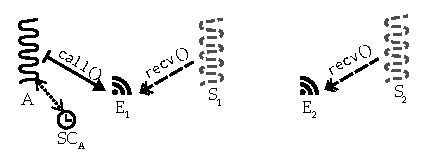
\includegraphics[width=\textwidth]{forward1}
        \caption{$A$ \call() $S_{1}$ over $E_{1}$.}
        \label{f:forward1}
    \end{subfigure}
    \begin{subfigure}[h]{0.8\textwidth}
        \centering
        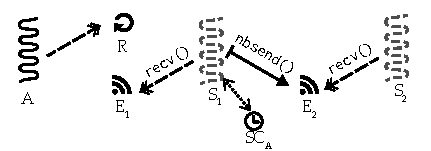
\includegraphics[width=\textwidth]{forward2}
        \caption{$S_{1}$ uses \nbsendrecv() to forward the request, and $A$'s resume 
            capability, to $E_{2}$, and
        wait for further messages on $E_{1}$.}
        \label{f:forward2}
    \end{subfigure}
    \begin{subfigure}[h]{0.8\textwidth}
        \centering
        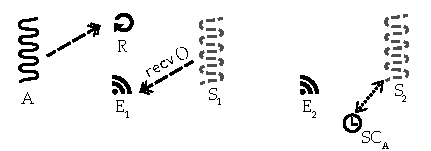
\includegraphics[width=\textwidth]{forward3}
        \caption{$S_{2}$ processes the request.}
        \label{f:forward3}
    \end{subfigure}
    \begin{subfigure}[h]{0.8\textwidth}
        \centering
        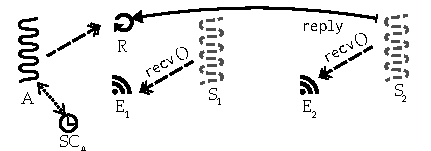
\includegraphics[width=\textwidth]{forward4}
        \caption{$S_{2}$ uses the \replyrecv() system call to reply to $A$ and block on
        $E_{2}$ again. }
        \label{f:forward4}
\end{subfigure}
\caption[IPC forwarding.]{IPC forwarding: client $A$ sends a request to passive server $S_{2}$ via a passive proxy $S_{1}$,
and the scheduling context passes from $A \rightarrow S_{1} \rightarrow S_{2} \rightarrow A$. See \Cref{f:legend-2} for the legend.}
\label{f:model-forward}
\end{figure}

\subsection{Flexible Resume Capabilities}

The final mechanism we introduce is the ability to transfer resume capabilities between servers. 
This means that a blocked thread can be forwarded to other threads, thus allowing the resume
capability to be moved. Note that this is explicitly not delegation: resume capabilities cannot be
copied.

\subsection{Notification Binding}

Recall from \cref{s:notification-binding} that notification objects can be bound to threads such that single-threaded servers can be 
constructed which receive \gls{IPC} messages and signals. We extend this mechanism with passive server
support by allowing scheduling contexts to be bound to notifications, such that the passive server
execute using the notification's scheduling context when processing interrupts or signals from other
threads. 

\section{Policies}
\label{sec:model-policies}

We now describe how different policies can be implemented by user-level systems using the 
existing mechanisms in seL4, combined with the new mechanisms of scheduling contexts,
scheduling context donation, directed yield, \gls{IPC} forwarding, and flexible resume capabilities.
First, we explain how different best-effort, rate-based and real-time tasks are compatible
with our model and describe their implementation. We subsequently explain how various different 
resource sharing policies and servers, with and without temporal isolation, can be constructed. 

\subsection{Scheduling policies}

\subsubsection{Best-effort threads}

Best-effort threads, scheduled round-robin, are compatible with our model, which maintains
compatibility with the previous, baseline \selfour scheduler.  Full scheduling contexts are the
mechanism to support best-effort threads, and by setting the budget and period to equal, system
designers can set a timeslice, which determines how long a specific scheduling context can be
executed upon before preemption.

More complicated, time-sharing schedulers can be built by a user level scheduler, using the directed
yield and ability to request the amount of time consumed by a specific scheduling context.

\subsubsection{Rate-limited threads}

Rate-limited threads simply have their scheduling contexts configured with
parameters that express the desired upper-bound on rate.  No other work is
required by the user: if there are no higher priority threads and the
rate-limited thread does not block, it will be runnable at the rate expressed
in the scheduling context.  Otherwise, the thread will be capped at the rate
specified, but cannot be guaranteed to get the entire rate allocation if there
are higher priority threads in the system, or if the priority of the
rate-limited thread is overloaded.

\subsubsection{Periodic, polling threads}

Threads that need to wake, poll for an event, and sleep again can be
implemented using the sporadic server mechanism, by  
setting threads' scheduling parameters appropriately. As long as the budget is
not full ($C\neq T$), the \yield system call can be used to block until the next replenishment
is available, as shown in \cref{list:polling}. However, this approach will only work if the amount of thread preemptions 
is known and the amount of extra sporadic replenishments is set correctly, as \yield sleeps until
the next available replenishment. If fragmentation occurs due to preemption and incorrect sporadic
replenishments, the polling thread will not wake at the start of every period. This could be
ameliorated by checking the time on wakeup, or using a different task model.  

\begin{listing}
  \begin{minted}{c}
      for (;;) {
          seL4_Word badge;
          seL4_Poll(notification_object, &badge);
          doJob();
          // sleep until next job is ready
          seL4_Yield();
      }
  \end{minted}
  \caption{Example of a polling task on \selfour.}
  \label{list:polling}
\end{listing}

\subsubsection{Sporadic threads}

Recall that sporadic threads wake due to an event such as an interrupt, then process the event and
go back to sleep. To constrain sporadic thread's execution times, they are given a maximum
inter-arrival time.
To build sporadic threads notifications can be used
with scheduling contexts, as displayed in \cref{list:model-sporadic}. In this case, if the
number of sporadic replenishments is not sufficient, the processing bandwidth may be artificially
limited by excessive preemptions, otherwise it will be $\frac{C}{T}$. 

\begin{listing}
  \begin{minted}{c}
      for (;;) {
          doJob();
          // sleep until next job is ready
          seL4_Word badge;
          seL4_Wait(notification_object, &badge);
      }
  \end{minted}
  \caption{Example of a basic sporadic task on \selfour.}
  \label{list:model-sporadic}
\end{listing}

\subsubsection{Time triggered threads}

Time-triggered threads, which wake up, do some processing, and go to sleep again until the next
period can be set up with a user-level timer driver in order to wake at exactly the right time.
Scheduling contexts can be combined with this approach to rate-limit time-triggered threads, but 
the exact amount of preemptions does not need to be known.
\cref{list:model-sporadic} also applies to this policy, where the notification object is configured to
receive periodic notifications from a timer service.

\subsection{Resource sharing policies}

\subsubsection{\gls{PIP}/\gls{BWI}}
\label{sec:model-pip-bwi}

\begin{figure}
    \centering
    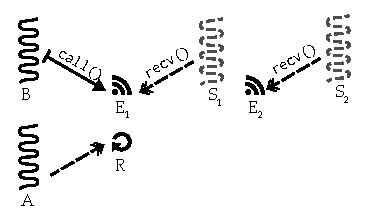
\includegraphics[width=0.7\textwidth]{pip}
    \caption[Example of proxying requests via a server.]{Example of proxying requests via a server that manipulates priorities before resource
    access, see \cref{f:legend-2} for the Legend.}
    \label{f:model-pip}
\end{figure}
 
\cref{f:model-pip} shows an example of a resource server ($S_{2}$) which proxies \gls{IPC} messages via
another server ($S_{1}$) to manipulate priorities according to some protocol before and after
requests. The policy works as follows: clients are given a badged capability to an endpoint,
$E_{1}$, on which to make requests on the resource server. $S_{1}$ receives requests, identifies 
the client via the badge, and manipulates $S_{2}$'s priority before forwarding the request to
$S_{2}$ over endpoint $E_{2}$. $S_{1}$ returns to wait on $E_{1}$, while $S_{2}$ processes the
request. If while $S_{2}$ is processing a request from $A$, and a higher priority thread $B$
preempts it and sends a request on $E_{1}$, $S_{2}$ can bump $S_{1}$'s priority again, and forward
$B$'s request to $S_{2}$, once again returning to wait on $E_{1}$ for further messages. When $A$'s
request is complete, $S_{2}$ enqueues a request on $E_{1}$, such that $S_{1}$ can readjust the
priority of $S_{2}$ according to the protocol, and reply to the original caller. Note that for this
method to work, $S_{1}$ must be the highest priority, and acts as a critical section for
manipulating priorities in the system.

Our description so far can be used to implement the \gls{PIP} or the \gls{OPCP}, depending on 
the logic used by the proxy-server $S_{1}$. This functions whether $S_{1}$ and $S_{2}$ are active or
not. In order to extend this protocol to bandwidth inheritance, a timeout fault handler would need
to be specified for both server threads, which could then bind the pending client's scheduling
context to the server to finish the request. 

\subsubsection{Best-effort Shared Server}
\label{sec:best-effort}

Best-effort systems have no timing requirements, so each thread in the system has a full \gls{SC}
with a budget and period the length of the timeslice. Threads are scheduled round-robin. To
implement such a system with our mechanisms, all server threads would be configured as active, and 
set to the ceiling priority of the clients. 

This policy does not provide temporal isolation, as the server executes on its own budget.  If one
client launches a denial of service attack on the server, depleting the servers budget, then other
clients are starved. 

While our resource sharing mechanisms do not rule out this policy, it is only suitable for
systems where all clients are trusted and the amount of requests each client makes is known \emph{a
priori}, or systems that have low temporal sensitivity.

\subsubsection{Migrating threads}

\composite~\citep{Parmer_10} solves the resource sharing model by using migrating 
threads (also termed stack-migrating \gls{IPC}).
On every \gls{IPC}, client execution contexts (and CPU reservation) transfer to a new stack running in the
server's protection domain, resulting in multi-threaded servers.

To implement migrating threads, \composite requires that every server have a mechanism for allocating stacks.
If no memory is available to allocate stacks, then the request is blocked.
This solution forces servers to be multi-threaded, and does not solve the problem of a clients budget expiring while the server is in a critical section, which is solved by providing atomic primitives that call the kernel.

A stack-spawning policy can be implemented using the mechanisms we have provided, similarly to
the \gls{PIP} implementation described above (\cref{sec:model-pip-bwi}), except the proxy
server spawns new worker threads instead of manipulating priorities. 
The stack-spawning proxy would also be at a lower priority than the worker threads, 
such that it would only be activated when all worker threads are busy.

An alternative policy is to build systems with a fixed number of server threads, all waiting on the
same endpoint. 
Like the best-effort policy, our model supports this approach but it is not required.

\subsubsection{Blocking Servers}

Some servers need to block in order to function: for example, servers providing \IO may need to wait
until an operation completes before replying to the client. Consider a disk server, where
clients make requests of the server to write data to the disk. The server makes the request to the
disk, but does not reply to the client until the device has signalled that \IO is complete. Rather
than blocking until the driver responds, preventing the server from taking on further requests, the
server can block on the endpoint and wait for the interrupt or further RPC requests. If an interrupt
comes in, the server runs the bound notification objects scheduling context to complete the
request.

Another option is to use multiple threads, with a passive thread for handling requests and an active
thread servicing interrupts, however this requires synchronisation between the threads within the
server.

\subsubsection{Server isolation}

We now describe how timeout handlers can be used to implement server isolation and other policies,
as previously introduced in \cref{sec:model-enforcement}. 

For our example consider a server shared between clients of different criticality, time sensitivity,
and trust, which provides an encryption service via \gls{AES}. 
Such a server processes data in blocks, and the \gls{WCET} of a request is a function of the 
amount of data to be encrypted. Such a server can be constructed transactionally in order
to render it preemptable: each block processed is considered a transaction. The server atomically
switches between two states each time it completes a block, effectively finishing one transaction
and starting another. The state the server is working on is always dirty, the previous is clean. 

By constructing the server in this way, a timeout handler can reset the server to the last clean
state if the passive server raises a timeout exception due to the client's \gls{SC} expiring. 
The timeout handler saves the server at a known checkpoint, and flips the server back to 
the known checkpoint. The handler can then reply to the client on the server's behalf, and return how
far through the request the server completed by reading it out of the last clean state. Invoking the
reply returns the scheduling context to the client, and the timeout handler blocks waiting for the
next request.

Other options are also available to the timeout handler, which is important as not all server
operations can be reset midway. The timeout handler can reply with an error to the client, 
not reply to the client at all, thereby preventing the client from making further requests, or 
bind a temporary scheduling context to the server to complete the request. 

\section{Summary}

In this chapter we have outlined our model for providing temporal isolation via scheduling and
resource sharing mechanisms. We introduce support for user-level
admission tests via a new control capability, and add processor reservations to the kernel in the form of scheduling contexts.  
Scheduling contexts differ from prior work in that they are decoupled from priority, thereby
avoiding priority inheritance on scheduling context donation, and by differentiating between passive and active servers we maintain policy freedom.

Finally, we outlined existing models for integrating real-time resource policies over \gls{IPC} and
show how scheduling-context donation combined with passive servers can be used to create trusted
servers with untrusted clients. 
Our model supports best-effort, migrating threads, or temporal isolation policies for resource sharing.

Timeout exceptions are provided which allow for user-defined enforcement policies, while the default
mechanism maintains isolation by preventing threads from executing for more than the share of processing
time represented by the scheduling contexts.

In the next section we will outline the implementation of our model in \selfour. 

\chapter{Implementation}
\label{chap:implementation}


In the previous chapter we presented our model for MCS mechanisms for a microkernel.
This section provides the deatils of the implementation in seL4.

% TODO should the seL4 background section go here?

Kernel changes include additions to the scheduler to support temporal isolation, scheduling contexts
objects, system call API changes and a new mechanism -- scheduling context donation -- which supports bandwidth inheritance.

These changes allow user-level to construct systems with combinations of best-effort and real-time threads.
We illustrate through example how threads can achieve resource sharing through reservation-per-thread, migrating threads or scheduling context donation policies.



\section{Objects}

We add two new objects to the kernel, \glspl{SCO} and resume objects. Additionally, we modify
the \gls{TCB} object although do not increase its total size. All three objects interact to
implement our mechanisms.

\subsection{Resume objects}
\label{s:resume}

Resume objects are introduced to track scheduling context donation over IPC path when \call is
used. Futher detail is provided in TODO.

\begin{description}
    \item[Caller] a pointer to the \gls{TCB} that is blocked on this reply object.
    \item[Prev,Next] pointers which track the call chain.
\end{description}

\subsection{Scheduling context objects}
\label{s:sco}

\glspl{SCO} are variable sized objects that represent access to a certain amount of time and
consist of a core amount of fields, and a circular buffer to track the consumption of time.
The core fields in a \gls{SCO} are as follows:

% TODO picture of scheudling context layout

\begin{description}
    \item[Period] The replenishment period.
    \item[Refills] A circular buffer of sporadic replenishments.
    \item[Consumed] The amount of cycles consumed since the last reset.
    \item[Core] The id of the processor this scheduling context grants time on.
    \item[TCB] A pointer to the thread this scheduling context is currently providing time to.
    \item[Reply] A pointer to the last resume object (see \cref{s:resume}) in a call chain where
        this scheduling context was donated.
    \item[Notification] A pointer to the notification object
    \item[Badge] A unique identifier for this scheduling context.
    \item[YieldFrom] Pointer to a \gls{TCB} that has yielded to this \gls{SCO}.
    \item[Head,Tail] Indexes to the circular buffer of sporadic replenishments.
    \item[Max] Maximum amount of replenishments for this scheduling context.
\end{description}

In addition to the core fields, scheudling contexts contain a variable amount of
\emph{replenishments}, which consist of a \emph{timestamp} and \emph{amount}. These are used for
both round-robin and sporadic threads.

%TODO discuss sporadic vs round robin, invocatinos on scheduling contexts

\subsection{Thread control block objects}

% TODO what is changed in TCBs

\section{Scheduling}

Now we discuss changes to the kernel scheduler and how the new \glspl{SCO} interact which the
scheduling algorithm to provide temporal isolation and asymmetric protection.
We show how best-effort and real-time threads are supported by these changes, and consider \emph{rate-based} threads -- which are essentially best-effort threads with a kernel-enforced bound on maximum rate.


\tikzstyle{decision} = [diamond, draw,
    text width=4.5em, text badly centered, node distance=3cm, inner sep=0pt]
\tikzstyle{block} = [rectangle, draw,
    text width=5em, text centered, rounded corners]
\tikzstyle{line} = [draw, -latex']


\begin{figure}
\begin{tikzpicture}[node distance = 3cm, auto]
    % place nodes
    \node[block]                      (entry)  {update kernel time};
    \node[block,    left of = entry]  (swi)    {enter kernel};
    \node[decision, below of = entry ](enough) {budget sufficient?};
    \node[block,    left of  = enough](tick)   {simulate tick};
    \node[block,    right of = enough](op)     {do kernel operation};
    \node[decision, below of = enough]    (sc)     {change SC?};
    \node[block,    left of  = sc]    (commit) {commit kernel time};
    \node[block,    right of = sc]    (rb)     {rollback kernel time};

    % place lines
    \path [line] (swi)    -- (entry);
    \path [line] (entry)  -- (enough);
    \path [line] (enough) -- node [near start, above] {no} (tick);
    \path [line] (enough) -- node [near start] {yes}(op);
    \path [line] (tick)   -- (sc);
    \path [line] (op)     -- (sc);
    \path [line] (sc)     -- node [near start] {yes} (commit);
    \path [line] (sc)     -- node [near start, above] {no}  (rb);
\end{tikzpicture}
\caption{Kernel structure}
\label{figure:tickless}
\end{figure}

We make changes to the scheduler and structure of the scheduler to support temporal isolation: we
convert the scheduler to tickless, add a release queue of threads waiting for budget replenishment
and introduce the invariant that threads without scheduling contexts are not eligible for
scheduling.

\subsection{Tickless}

We convert \selfour from a tick-based to a tickless kernel in order to reduce preemptions and
improve scheduling precision, as discussed in \Cref{sec:tick-v-tickless}.
As \selfour is non-preemtible (save for explicit preemption points in a few long-running
operations), tickless kernel design is non-trivial, as preemption interrupts cannot interrupt the
kernel itself.

The main change required to the existing scheduler is the addition of a \emph{release queue} per
processing core. If a
preempted thread does not have any available replenishments, the kernel removes the thread from the
ready queue to the release queue, retaining the invariant for the ready queue, which the release
queue is charaterised as holding all threads that would be runnable but are presentingly out of
budget. The queue is ordered by the timer when the next replenishment is available.

On kernel entry (except on the IPC fastpath, which never leads to an SC
change or scheduler invocation) the kernel updates the current
timestamp and stores the time since the last entry. This is required as when preemption occurs, the
preemptor is charged for the time since the kernel entry. Without knowing if the kernel entry will
trigger a thread switch in advance, the kernel must record the time for each entry. However, if the
recorded timestamp is not acted upon, the time is rolled back to the previously recorded value.

After recording the timestamp, the kernel then checks
whether the thread has sufficient budget to complete the kernel
operation, using a fixed estimate of double the kernels \gls{WCET}.
If the available budget is insufficient, the kernel pretends the timer has already fired,
resets the budget and adds the thread to the release queue. If the entry was due to a system call
,the thread will retry that call once it wakes with further budget.
Once the thread is awoken it will retry the system call

This adds a new
invariant, that any thread in the scheduling queues must have enough budget to exit the kernel.
It makes the scheduler precision equal twice the kernel's WCET, which for
seL4 is known (unlike any other protected-mode OS we are aware of).
This invariant is required as it simplifies the kernel design and actually minimises the WCET: when
a
thread runs out of time it may need to raise a timeout exception resulting in delivering an IPC to a
timeout handler.By requiring that anything in the scheduler queue, or any endpoint queue, must have
enough budget to wake up we avoid needing to potentially raise timeout exceptions on many wakeup
paths in the kernel.

Threads are only charged when the scheduling context changes, in order to avoid
reprogramming the timer which can be expensive on many platforms. %(\autoref{s:timer-reprogram}).
If there is no SC change, the timestamp update is rolled back by subtracting the
stored consumed value from the timestamp.
\autoref{figure:tickless} illustrates the structure of this kernel design.

\subsection{Priority queues}

Priority queues for both scheduling algorithms are implemented as ordered lists, with $O(n)$ insertion and removal complexity.
The most frequent operation on the lists is to remove the head, which is $O(1)$.
We choose a list over a heap for increased performance and reduced verification burden.

A list-based priority queue out performs a heap-based priority queue for small $n$ in our implementation up to around $n = 100$.
This $n$ is larger than one would expect in a traditional \gls{OS}, where heap implementations are array-based in contiguous memory with layouts optimised for cache usage.
However, in order to provide isolation and confidentiality, \selfour kernel memory is managed at user-level, as discussed in %TODO{section}.
Consequently, to put a \selfour kernel object into a heap, the pointers for the heap implementation must be contained within the object, which could be anywhere in memory as chosen by the user.
This means that \selfour heap implementations are non-contiguous, and must be pointer based, resulting in a much larger cache footprint with worse performance than an array-based approach.

verification.
Of course, even if the heap implementation is slower, given a sufficient number of tasks a heap will scale better than a list.
However, we do not expect systems to run a large amount of real-time tasks, as \selfour target applications generally run virtualised Linux along-side a few critical real-time tasks.
Additionally, the reduced complexity of a list compared to a heap will result in faster verification, so consequently a list implementation looks favourable.

%TODO{Link to eval}
\subsection{Admission}

As established in section \Cref{sec:model-admission}, admission tests for reservations are considered policy to be implemented by user-level.

In the current design, we control the creation of scheduling contexts by conveying the authority to populate their parameters into a single capability per processor.
Each processor has a scheduling control capability, all of which are given to the root task on initialisation.
Scheduling contexts can be created by any task, using standard seL4 conventions to create an object, which result in a scheduling context with all parameters are set to 0.
The implication is that tasks in the system with access to memory can only create empty reservations.
While an empty reservation can be bound to a thread, since the reservation contains no budget that thread will never be eligible to run.

In order to populate the parameters of a scheduling context, one must invoke a new capability: the scheduling control capability for the core that the thread is intended to run on.
Only a single copy of this capability is available per processor in the system, so the population of scheduling contexts with parameters is restricted to processes with access to those capabilities, which can conduct admission tests as per user-level policy.

\subsection{Scheduling Contexts}
\label{sec:schedcontext}

We introduce a new kernel object type, scheduling contexts, which act as processor reservations and contain sporadic task parameters.
Scheduling contexts encapsulate processor time reservations, derived from sporadic task parameters: min-period ($T$) and a set of replenishments which is populated from an original execution budget ($C$), representing the reserved rate reserved rate ($U$) = $\frac{C}{T}$.
The execution budget will be populated with the \gls{WCET} for \gls{HRT} tasks, and a max-rate for \gls{SRT} and rate-based tasks.

Scheduling contexts are connected to one thread at a time.
A thread is not permitted to execute for more time than that represented in the scheduling context.
Threads without scheduling contexts are not runnable.

Scheduling contexts also form part of the accounting mechanism: the amount of budget a thread has remaining, and when the budget is due to be recharged, are stored in the scheduling contexts.
\Cref{tab:sched_context} displays a summary of the main fields stored in a scheduling context object.

The method \texttt{seL4\_SchedControl\_Configure} is used to set the parameters on a specific scheduling context.
It taskes a \texttt{budget}, \texttt{period}, \texttt{num\_extra\_refills} and \texttt{badge}.

\subsection{Replenishments}
\label{sec:replenishments}

Scheduling contexts contain a circular buffer for sporadic task replenishments.
Each replenishment has an amount of time that stands to be replenished, and the absolute time from when that replenishment can be used, as shown in \cref{tab:refill}.
When \texttt{seL4\_SchedControl\_Configure} is called on an inactive scheduling context, the amount is set to the budget and the replenishment time to the current time.
At all times, the sum of the amounts in the replenishment buffer is equal to the configured budget.
The maximum size of this buffer is statically configurable, and the minimum size is one.
Users can specify the amount of extra refills a scheduling context can have, up to the static maximum.

Scheduling contexts with zero extra refills behave like polling servers (\cref{p:polling-servers}), otherwise they behave as sporadic servers (\cref{p:sporadic}), allowing application developers to tune the behaviour of threads depending on their preemption levels and execution durations.

The algorithms to manage replenishments are taken from \citet{Danish_LW_2011}, with adjustments to support periods of 0 (for round robin threads) and to implement a minimum budget.
Whenever the current scheduling context is changed, \texttt{check\_budget} as shown in Listing \ref{list:check-budget} is called to bill the amount of time consumed since the last scheduling context change.
`check\_budget`
If the budget is not completely consumed by \texttt{check\_budget}, \texttt{split\_budget} as shown in Listing \ref{list:split-check} is called to schedule the subseqeunt refill for the chunk of time just consumed.
If the replenishment buffer is full, or the amount consumed is less than the minimum budget, the amount used is merged into the next replenishment.
The scheduling context being switched to has \texttt{unblock\_check} Listing (\ref{list:unblock-check}) called on it, which merges an replenishments that are already available, avoiding unneccessary preemptions.

When \texttt{seL4\_SchedControl\_Configure} is called on an active scheduling context, the refills are adjusted to reflect the new budget and period but respect the sliding window constraint.

Round-robin threads have full reservations: $T = C$, entitling them to 100\% of the processor but subject to preemption every time $C$ is used.
Clearly we don't want to track replenishments for round-robin threads, so the kernel detects if round robin scheduling contexts when \texttt{seL4\_SchedControl\_Configure} is called, and sets the period to 0.
This avoids much special casing in the replenishment code, as round-robin threads are always ready (we always add 0 to the replenishment time).

\begin{lstlisting}[frame=single,language=c,caption=Check budget routine.,label=list:check-budget,float=htpb]
uint_64_t check_budget(sched_context_t *sc, uint64_t usage) {
  while (head_refill(sc).amount <= usage) {
    // exhaust and schedule replenishment
    old_head = pop_head(sc);
    usage -= old_head.amount;
    old_head.time += sc->period;
    add_tail(sc, old_head)
  }

  /* handle budget overrun */
  if (usage > 0 && sc->period > 0) {
    // delay refill by overrun
    head_refill(sc).time += usage;
    // merge replenishments if time overlaps
    if (refill_size(sc) > 1 &&
        head_refill(sc).time + head_refill(sc).amount
        >= refill_next(sc).time) {

      refill_t old_head = pop_head(sc);
      head_refill(sc).amount += old_head.amount;
    }
  }
}
\end{lstlisting}

\begin{lstlisting}[frame=single,language=c,caption=Split check routine.,label=list:split-check,float=htpb]
void split_check(sched_context_t *sc, uint64_t usage) {
  uint64_t remnant = head_refill(sc).amount - usage;
  if (remnant < MIN_BUDGET && refill_size(sc) == 1) {
    // delay entire replenishment
    // refill too small to use and nothing to merge with */
    head_refill(sc).time += sc->period;
    return;
  }

  if (refill_size(sc) == sc->refill_max || remnant < MIN_BUDGET) {
    // merge remnant - out of space or its too small
    pop_head(sc);
    head_refill(sc).amount += remant;
  } else {
    // split the head refill
    head_refill(sc).amount = remnant;
  }

  // schedule the used amount
  refill_t split;
  split.amount = usage;
  split.time = head_refill(sc).time + sc->period;
  add_tail(sc, split);
}
\end{lstlisting}

\begin{lstlisting}[frame=single,language=c,caption=Unblock check routine.,label=list:unblock-check,float=htpb]
void unblock_check(sched_context_t *sc) {
  if (!head_refill(sc).time > now)) {
    return;
  }

  head_refill(sc).time = now;
  // merge available replenishments
  while (refill_size(sc) > 1) {
    if (refill_next(sc).time < now + head_refill(sc).amount) {
      refill_t old_head = pop_head(sc);
      head_refill(sc).amount += old_head.amount;
      head_refill(sc).time = now;
    } else {
      break;
    }

    if (head_refill(sc).amount < MIN_BUDGET) {
      // second part of split_check can leave refills
      // with less than MIN_BUDGET amount.
      // detect them here and merge.
      refill_t old_head = pop_head(sc);
      head_refill(sc).amount += old_head.amount;
    }
}
\end{lstlisting}


\subsection{Task model}

We extend the seL4 API with support for real-time and rate-based tasks, while maintaining support for round-robin, best-effort tasks.
In this section we present how our mechanisms support each type of task, and how user-level should configure them.

\subsubsection{Best-effort threads}

Best effort threads, scheduled round-robin, are compatible with our model.
In the original seL4 kernel, best effort threads would be scheduled for CONFIG\_TIME\_SLICE ticks, before being taken from the start of their run queue and placed at the end of the run queue.
This was sufficient for round-robin scheduling.

Scheduling contexts for best-effort threads are assigned an equal budget and period, with the value set to the desired round-robin time slice for the thread.
Since the budget and period of threads configured in this fashion are equal, when the budget expires it will be immediately replenished as the period has passed already.
However, replenishment places a thread on the end of its run queue, thereby implementing round-robin scheduling, as any other thread in the queue will be scheduled first.
This approach minimises the amount of code required and should result in a fast scheduler, with no special cases for best-effort versus real-time threads.
Of course, populating scheduling context parameters as such entitles best-effort threads to an effective 100\% share of the CPU, so it should only be used at low priorities.
Additionally, real-time threads and best-effort threads should not run at the same priority.

\subsubsection{Rate-limited threads}

Rate-limited threads simply have their scheduling contexts configured with parameters that express their desired bound on rate.
No other work is required by the user: if there are no higher priority threads and the rate-limited thread does not block, it will be runnable at the rate expressed in the scheduling context.
Otherwise, the thread will be capped at the rate specified, but cannot be guaranteed to get the entire rate allocation if there are higher priority threads in the system, or if the priority of the rate-limited thread is overloaded.
%TODO{ talk about sporadic refill parameter}

\subsubsection{Real-time threads}

Real-time threads are more complicated than rate-limited or best-effort threads, as the concept of a sporadic job, including job release time and job completion, need to be supported by the kernel API.

We define the initial job release as when a thread is resumed: the available budget is set to the total budget in the reservation for that thread.

Job completion is more complicated.
As described in section \Cref{sec:sporadic-task-model}, job completion occurs when a job blocks waiting for the next job to be released.
Any budget left by the current job is released as slack into the system, which means the available reservation budget drops to 0.
If a job is time-triggered, such that it only relies on time for job release, then next job will be released once the period has passed.
If a job is event-triggered, then the next job should be released once the period has passed \textit{and} an external event occurs, such as an interrupt.

Simply defining job completion as when a task blocks is not sufficient as jobs can also block for other reasons, like polling I/O, or waiting for an asynchronous server.
Unintentionally completing a job by blocking is incorrect, as it would result in real-time threads receiving less processing time than they have reserved.

One design option we considered was to use the yield system call to complete the current job.
However this approach would not enable a thread to receive a notification on job release, requiring more system calls to retrieve notifications.

\begin{lstlisting}[frame=single,language=c,caption=Example of a basic sporadic real-time task on sel4.,    label=list:sporadic-sel4]
    for (;;) {
        // job is released
        doJob();
        // job completes before deadline or is postponed by CBS
        // sleep until next job is ready
        seL4_Word badge;
        seL4_Wait(bound_async_endpoint, &badge);
    }
\end{lstlisting}

% TODO background on endpoints, endpoint binding on backgournd sel4 section to support this.
Instead, we use asynchronous endpoints to implement sporadic jobs on seL4, which unifies jobs to be completed and release with notifications, reducing the amount of system calls required.
Currently, asynchronous endpoints can be bound to a thread, which enforces a one-to-one relationship be  tween the bound thread and the bound endpoint.
The current semantics of async endpoint binding allow threads to wait on a synchronous endpoint and receive notifications from their bound async endpoint at the same time.
Due to implementation complexities, no thread but the bound thread is permitted to wait on the bound endpoint.
However, in practice, threads only ever wait on a separate synchronous endpoint, not the bound endpoint.
As a result, we use this operation to implement job completion.

The new semantics are simple: waiting on the bound asynchronous endpoint completes the current job.
The next job is released when a notification arrives on the endpoint.
If the budget has not been replenished at this point, the thread will not be runnable until it is.
This design allows a simple distinction between standard blocking, and blocking to complete the current job.
A code example of what real-time threads look like on seL4 is shown in Listing \ref{list:sporadic-sel4}.

Time-triggered jobs have an additional semantic, as the kernel will send a notification to the asynchronous endpoint when the period passes to release the next job.
This is a conscious design choice: it would be possible for users to implement time-triggered jobs using a user-level timer driver.
In that case the kernel could treat all real-time jobs as event-triggered jobs.
However, since the kernel at this point already contains a trusted timer driver to support the enforcement mechanism, it is impractical to require users to provide a second trusted timer driver for periodic, real-time threads.
This also reduces overhead for time-triggered jobs, as less context switches are required for job release.

Best-effort and rate-limited threads in practise run one real-time job, as they never complete their current job.
If a real-time job does not complete before its budget expires, then it will be rate-limited, preserving temporal isolation.

\subsection{Compatibility with the domain scheduler}

While the real-time amendments to the scheduler are compatible with the domain scheduler, either the domain scheduler or the real-time amendments should be used for real-time scheduling.
This is because domains are non-preemptive and as a result can only be used for non-preemptive real-time scheduling, where domain parameters exactly match real-time scheduling parameters.
Using more than one domain when preemptive real-time scheduling is will result in missed deadlines.



\section{Resource Sharing}

Thread communications in seL4 take place via the IPC mechanism, which we alter to support scheduling context donation.
In this section we will address changes to the system calls used to send and receive IPC messages to implement scheduling context donation.
% more
We then illustrate through example how reservation-per-thread, thread-migrating IPC and scheduling context donation can be built with the new \gls{API}.

\subsection{Endpoints}

\gls{IPC} in seL4 is conducted through endpoints, which do not denote a specific receiving or sending thread, but act as arbitrary communication endpoints.
Any thread with an endpoint capability can send or receive messages on that capability: if two threads send and receive messages on the same endpoint, then a communication rendezvous occurs and a message is send.

Endpoints are either synchronous: sending a message on a synchronous endpoint blocks the sender until the message is received, and in the case of multiple messages a queue of messages to be processed forms on the endpoint.
As a result, IPC over synchronous endpoints triggers a thread switch.
Messages on asynchronous endpoints do not block the sender, and are combined instead of forming a queue.
We use IPC on synchronous endpoints to donate scheduling contexts, while asynchronous communication is expected to occur between threads with their own reservations.

\subsection{Reply objects}

%TODO{Reply objects}

\begin{table}
    \centering
    \begin{tabular}{|>{\texttt\bgroup}l<{\egroup} | p{6cm} |} \hline
        \textnormal{\textbf{Field}} & \textbf{Description} \\\hline
         tcb\_t *tcb    & The calling thread that is blocked on this reply object. \\\hline
         void *prev & 0 if this is the start of the call stack, otherwise points to the previous reply object in the call stack. \\\hline
         void *next & Either a pointer to the scheduling context that was last donated using this reply object, if this reply object is the head of a call stack (the last caller before the server) or a pointer to the next reply object in the chain. 0 if no scheduling context was passed along the chain.\\\hline
    \end{tabular}
    \caption{Fields in a reply object.}
    \label{tab:reply_object}
\end{table}


\subsection{Donation semantics}

A synchronous message in seL4 can be sent by using the following system calls on a synchronous endpoint capability:

\begin{itemize}
	\item \send blocks until the message is received by another thread, then the sender continues execution.
	\item \nbsend only performs the send if the receiver is already waiting, otherwise it fails (although the client cannot tell which behaviour occurred).
	\item \call sends a message to another thread and blocks until a reply is received back.
\end{itemize}

\call is a special case: when \call is executed the kernel manufactures a special, single-use capability (referred to as the reply cap) which the callee invokes to reply to the message.
The presence of the reply capability guarantees that a blocking thread is present to receive a reply.
The reply capability is actually a thread object, not the endpoint, so reply messages are not conducted through an endpoint.
Replies can be sent with the following two system calls:

\begin{itemize}
	\item \reply sends a reply message and blocks the replying thread until the message is received.
	\item \replywait sends a reply and then blocks on an endpoint argument to the system call until another message is received.
\end{itemize}

To implement scheduling context donation, we augment the system call API as follows:

\begin{itemize}
	\item \call (altered) between a caller that has a scheduling context and a callee that does not have a scheduling context donates the callers scheduling context to the callee. If the callee has a scheduling context then donation does not occur. The callee runs at its own priority, as per \gls{HLP}.
	\item \replywait (altered) to a thread without a scheduling context donates the scheduling context to subject of the reply.
    \item \sendwait (new), which allows a thread to send a message and donate a scheduling context to an endpoint or reply cap, then wait on another endpoint.
\end{itemize}

Scheduling context donation does not occur on \send, \nbsend or \reply,  as the sender cannot continue to execute without a scheduling context, and without receiving one from another thread the sender is blocked.
These system calls are not unusable, but should should be used between threads who have their own scheduling contexts.
If a thread attempts to use \send, \reply or \nbsend to communicate to a thread without a scheduling context, the communication will block.

\begin{figure}
\centering
    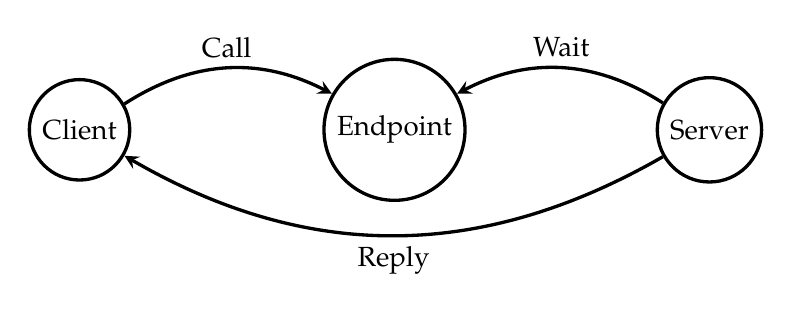
\begin{tikzpicture}[node distance=4cm,on grid,>=stealth,very thick,initial text=Event]
        \node[state] (client)   {Client};
        \node[state] (endpoint) [right=of client] {Endpoint};
        \node[state] (server)   [right=of endpoint] {Server};
        \path[->]
            (client) edge [bend left]  node [above] {Call} (endpoint)
            (server) edge [bend right] node [above] {Wait} (endpoint)
            (server) edge [bend left]  node [below] {Reply} (client)
        ;
    \end{tikzpicture}
\caption{Client-server scenario with \call and \replywait and a synchronous endpoint.}
\label{fig:client-server-endpoint}
\end{figure}

\begin{figure}
\centering
    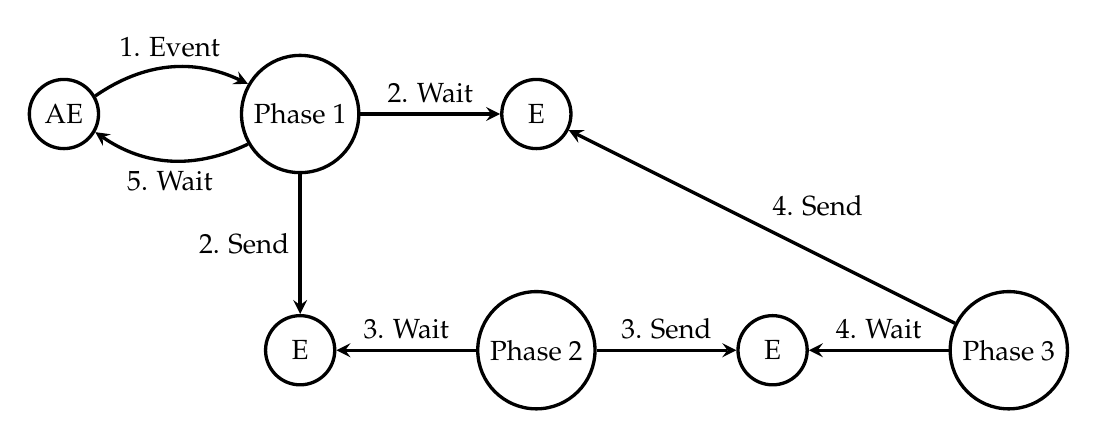
\begin{tikzpicture}[node distance=3cm,on grid,>=stealth,very thick,initial text=Event]
        \node[state] (async_endpoint)                      {AE};
        \node[state] (phase_1)   [right of=async_endpoint] {Phase 1};
        \node[state] (endpoint0) [right of= phase_1]         {E};
        \node[state] (endpoint1) [below of= phase_1]         {E};
        \node[state] (phase_2)   [right of= endpoint1]      {Phase 2};
        \node[state] (endpoint2) [right of= phase_2]        {E};
        \node[state] (phase_3)   [right of= endpoint2]      {Phase 3};
        \path[->]
            (async_endpoint) edge [bend left]  node [above] {1. Event} (phase_1)
            (phase_1)        edge [bend left]  node [below] {5. Wait}  (async_endpoint)
            (phase_1)        edge              node [above] {2. Wait}  (endpoint0)
            (phase_1)        edge              node [left]  {2. Send}  (endpoint1)
            (phase_2)        edge              node [above] {3. Wait}  (endpoint1)
            (phase_2)        edge              node [above] {3. Send}  (endpoint2)
            (phase_3)        edge              node [above] {4. Wait}  (endpoint2)
            (phase_3)        edge              node [above right] {4. Send}  (endpoint0)
        ;
    \end{tikzpicture}
\caption{Data-flow scenario with endpoints: AE indicates an asynchronous endpoint through which an event occurs, E indicates a synchronous endpoint. Numbering indicates event ordering: a Send and Wait with the same number occur in one system call.}
\label{fig:dataflow-endpoint}
\end{figure}

\Cref{fig:client-server-endpoint} and \Cref{fig:dataflow-endpoint} illustrate the client-server and data-flow scenarios with endpoints, using \call, \replywait and \sendwait.
The cycle in the data-flow scenario is required in order to donate the scheduling context back to the source of the event: otherwise, after one iteration, phase 1 has no reservation budget to execute the next event on.

\subsubsection{SendWait}

Introducing \sendwait into the kernel can lead to a long-running operation if the send part of the system call, when called on a synchronous endpoint, is allowed to block.
\Cref{fig:sendwait-chain} depicts this scenario.
This situation can be avoided if \sendwait is only allowed to occur if the send stage is non-blocking: the rendezvous partner must already be blocking on the endpoint that the send is called on.
This is not a problem when the \sendwait is called on a reply cap: the presence of the reply cap guarantees a thread is blocked waiting for a reply.
As a result, \sendwait when called on a synchronous endpoint will succeed if the receiver is ready and waiting.
Note that this long-running operation is not a problem with the existing \call, as the presence of the reply cap guarantees that earlier threads in the chain are blocked, preventing the long-running operation.

\begin{figure}
\centering
    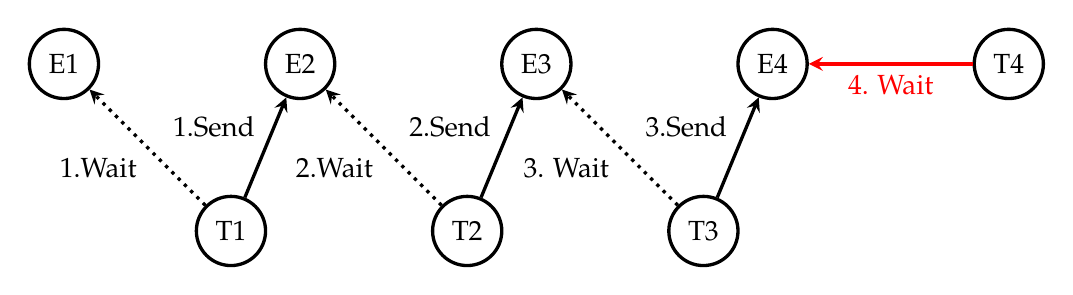
\begin{tikzpicture}[node distance=3cm,on grid,>=stealth,very thick,initial text=Event]
        \node[state] (e3)              {E1};
        \node[state] (e2) [right of=e3] {E2};
        \node[state] (t2) [below right of=e3] {T1};
        \node[state] (e1) [right of=e2] {E3};
        \node[state] (t1) [right of=t2] {T2};
        \node[state] (e0) [right of=e1] {E4};
        \node[state] (t0) [right of=t1] {T3};
        \node[state] (tx) [right of=e0] {T4};

        \path[->]
             (t0) edge          node [above left] {3.Send} (e0)
             (t0) edge [dotted] node [below left] {3. Wait} (e1)
             (t1) edge          node [above left] {2.Send} (e1)
             (t1) edge [dotted] node [below left] {2.Wait} (e2)
             (t2) edge          node [above left] {1.Send} (e2)
             (t2) edge [dotted] node [below left] {1.Wait} (e3)
             (tx) edge [color=red] node [below] {4. Wait} (e0)
        ;
    \end{tikzpicture}
\caption{A \sendwait triggering a long-running kernel operation. Threads T1, T2 and T3 call \sendwait on endpoint pairs (E1, E2), (E2, E3) and (E3, E4) respectively, however each thread blocks on the send. Finally T4 waits on E4, triggering a chain of messages that the kernel would have to process if this pattern were permitted.}
\label{fig:sendwait-chain}
\end{figure}

\subsubsection{Server/Activity blocking}

If a phase or server blocks waiting on input from another endpoint, messages can accumulate on the endpoint that donation occurs through.
This could be input from a device, or input from another task with its own reservation.
In this case, the request from the client with the highest priority should be serviced first to maintain real-time guarantees.
This requires endpoint queues to be ordered, which increases the complexity of a non-fastpath IPC to $O$(number of threads)\footnote{By using a heap this could be reduced to $O$(log$_{2}$(number of threads)), however we have conducted measurements previously establishing that a pointer-based list implemented in seL4 beats a pointer-based heap for up to and beyond 100 threads.}.
IPC ordering only needs to be applied to one side of the rendezvous process: either when the message is enqueued or when it is dequeued.

In some models, a server may wish to avoid blocking on input, but instead to issue an asynchronous request and continue to service other clients requests.
In the verified seL4 kernel, a server would achieve this using the asynchronous endpoint binding mechanism or using a multi-threaded approach with one thread per client.
The latter implementation is compatible with the scheduling context design, and will be explained in \Cref{sec:multithread}.
However the former approach is not compatible with passive servers running on clients scheduling contexts.
If scheduling context donation is not used, and the server has its own scheduling context, then the asynchronous endpoint binding approach remains viable.

\subsubsection{Revoking a server}

What happens if a server is revoked while executing on a clients scheduling context?
Since the kernel does not track the `home' of a scheduling context, it is not possible to return the scheduling context to the calling thread.
Currently the scheduling context will be disconnected from the server, and not returned to the caller.

In real scenarios, this revocation should only occur if the sub-system is being torn down so this is not a problem.
Otherwise, the scheduling context object is still valid: but it won't have any threads associated with it.
A supervisor thread could be set up to reset the scheduling contexts of any threads that have lost theirs if a server goes down.
Generally, if a server goes down in the middle of a request, action must be taken to restart the server and fix the client anyway so restoring the scheduling context must be incorporated in the protocol.
Note that if the server goes down the reply cap is also lost: so in the current seL4 design restarting the server and replying to the client is already impossible.

\subsection{Temporal Exceptions}

Threads can register a synchronous endpoints for two different types of temporal faults: deadline faults and budget faults.
In the former cause, a temporal fault is generated if the budget of a scheduling context expires while it is not home.
In the latter case, the current job is not completed before the deadline passes.
Both faults are optional and no fault message will be delivered if the respective endpoint is not set.

\subsection{Helping}

We introduce a new mechanism to the kernel -- helping -- which implements bandwidth inheritance as discussed in \Cref{sec:bandwidth-inheritance}.
Helping only occurs if a scheduling context runs out of budget, no temporal fault handler is registered for the current thread, and another thread has attempted to contact the stuck server.
Bandwidth inheritance is supported to allow shared servers and phases to remain single threaded.

\begin{figure}
\centering
    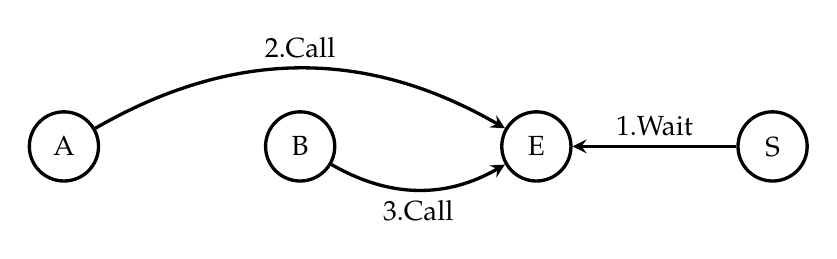
\begin{tikzpicture}[node distance=3cm,on grid,>=stealth,very thick]
        \node[state] (a)              {A};
        \node[state] (b) [right of=a] {B};
        \node[state] (e) [right of=b] {E};
        \node[state] (s) [right of=e] {S};
        \path[->]
             (a) edge [bend left]  node [above] {2.Call} (e)
             (b) edge [bend right] node [below] {3.Call} (e)
             (s) edge              node [above] {1.Wait} (e)
        ;
    \end{tikzpicture}
\caption{Client A makes a request from server S on endpoint E. A's scheduling context is donated from A to S. The budget expires while S is executing the request, blocking S from servicing other requests. Another Client, B, attempts to make a request but finds S blocked.}
\label{fig:budget-expiry}
\end{figure}

We explain the helping mechanism with reference to \Cref{fig:budget-expiry}.
$A$ sends an IPC to $S$ via endpoint $E$, and scheduling context donation occurs: $S$ is now running on $A_{sc}$.
As part of the donation process, a pointer to $S_{tcb}$ is stored in $E$, as the help-target.
$A_{sc}$ expires, and $B$ becomes runnable, issuing a request to $S$ via $E$.
Since no other threads are waiting to receive messages on $E$, $B$ inspects the state of the help-target, and finds that $S$ is running on expired scheduling context, $A_{sc}$.
$S$ inherits $B_{sc}$ in order to finish its request.
When $S$ replies to $A$, $A_{sc}$ is returned to $A$, and $S$ picks up $B$'s request from the IPC message queue, inheriting $B_{sc}$.

If $B_{sc}$ also expires, then it will be returned to $B$ and $B$ is removed from the endpoint queue.
When $B_{sc}$ is recharged, it can restart the operation.
This approach avoids large dependency chains in the system, and is acceptable as helping will never be triggered by \gls{HRT} threads, and is intended for use by rate-based threads and \gls{SRT} threads.

\subsubsection{Nested helping}

With the presence of nested servers, budget expiry can also occur and is more complicated.
Note that in the data-flow scenario, nested budget expiry is not possible as once a phase is executed and the scheduling context passed on, that phase is ready to execute another request immediately.
Nested budget expiry is illustrated in \Cref{fig:nested-budget-expiry}.

\begin{figure}
\centering
    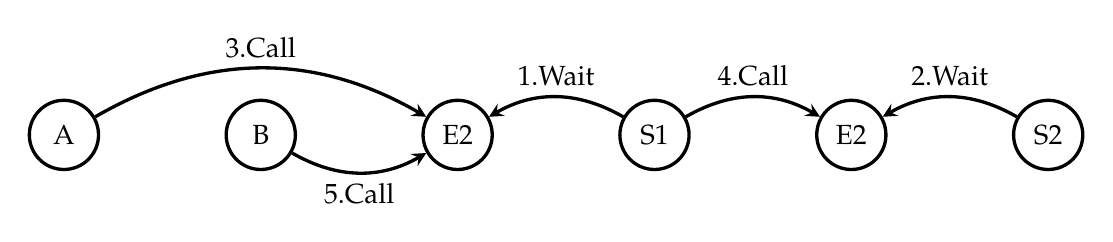
\begin{tikzpicture}[node distance=2.5cm,on grid,>=stealth,very thick]
        \node[state] (a)              {A};
        \node[state] (b) [right of=a] {B};
        \node[state] (e1) [right of=b] {E2};
        \node[state] (s1) [right of=e1] {S1};
        \node[state] (e2) [right of=s1] {E2};
        \node[state] (s2) [right of=e2] {S2};
        \path[->]
             (a) edge  [bend left]  node [above] {3.Call} (e1)
             (b) edge  [bend right] node [below] {5.Call} (e1)
             (s1) edge [bend right] node [above] {1.Wait} (e1)
             (s1) edge [bend left]  node [above] {4.Call} (e2)
             (s2) edge [bend right] node [above] {2.Wait} (e2)

        ;
    \end{tikzpicture}
\caption{Clients A makes a request to server S1 on endpoint E1. S1 receives A's request first, and makes a nested request to another server, S2. A's scheduling context is donated from A to S1 to S2, but the budget expires while S2 is executing.  A's budget expires while S is executing on it, blocking S from servicing other requests. Client B now makes a request, and finds S1 blocked.}
\label{fig:nested-budget-expiry}
\end{figure}

This problem can also be solved through helping by following the chain of help-target TCBs and passing the scheduling context through the chain.
This requires the addition of preemption points as it introduces a long-running operation.
If the operation is preempted, the chain search will be abandoned until the thread is scheduled again, at which point the \call will be restarted (since anything could happen during the preemption -- the scheduling context for the server may be replenished).

\subsection{Server and activity initialisation}

Except for systems using the reservation-per-thread model, where a scheduling context is assigned for each thread in the system, shared servers and activities are passive: they do not have their own scheduling context.
However, without a scheduling context these threads are not runnable, so how can one initialise a passive thread?

Two options are available using the new mechanisms: dedicated initialisation reservations, or helping.
Dedicated reservations involve resuming a thread with a reservation set purely for its initialisation phase.
The thread transfers the reservation back to the initialiser with a \sendwait call once it is ready to receive messages.

The helping approach operates by leveraging the helping mechanism and removes the requirement that a dedicated reservation be created purely for initialisation: instead, the initialiser passes its own reservation directly to the passive component.
To achieve this, a new kernel invocation is provided, \texttt{seL4\_Endpoint\_SetHelpTarget}, which allows the help target of an endpoint to be set.
To initialise a thread the initialiser can \call the server, thus donating its scheduling context to that thread via the helping mechanism.
The server can then \replywait to the initialiser, and it is now blocked waiting for the first client.

\subsection{Fastpath}

seL4 has an optimised fastpath that is executed for \call and \replywait.
As the semantics of these system calls have been altered, the impact on the fastpath has to be assessed.
The conditions to hit the fastpath currently are:
\begin{enumerate}
    \item the message arguments must fit into the scratch registers of the calling convention ($\leq$ 2 for x86, $\leq$ 4 for arm),
    \item the message must be sent on a synchronous endpoint,
    \item the receiver must be higher or equal priority,
    \item the receiver must be blocking on the endpoint,
    \item the message must be sent via a \call or \replywait.
\end{enumerate}
All of these conditions are performance optimisations: if we \call to a lower priority thread the scheduler would need to be invoked to check there are no other runnable threads at a higher priority than the receiver.

The addition of scheduling contexts raises adds a new condition to the fastpath:
\begin{enumerate}
    \setcounter{enumi}{5}
    \item the scheduling context must not change.
\end{enumerate}
When the current scheduling context changes, the time needs to be read to bill the previous scheduling context and an interrupt set for the budget expiry of the new scheduling context.
Adding these operations to the fastpath would slow it down greatly, as access to the timer device is expensive.
Consequently, the fastpath is aborted if the current scheduling context would change.

Scheduling context donation \emph{does} occur on the fastpath, as it only adds to writes.
Checking if the scheduling context will change adds 2 reads, and the donation takes 5 writes.

In future we will add a fastpath for \sendwait.

\subsection{Examples}

This chapter so far has outlined the various mechanisms added to the kernel to support resource sharing.
In this section we demonstrate how these mechanisms can be used to support different system policies for resource sharing.

\subsubsection{Reservation-per-thread}

Recall from \Cref{sec:reservation-per-thread} that in this model, clients and servers have their own reservations.
The reservation-per-thread model is the most simple to implement: all components in a system are assigned their own scheduling context with sufficient parameters.
If a shared resource runs out of budget, any clients will be blocked until the budget is recharged.
While independent threads in this example are temporally isolated from each other, threads sharing resources servers using reservation-per-thread are not temporally isolated.

\subsubsection{Migrating threads}

\begin{figure}
    \centering
    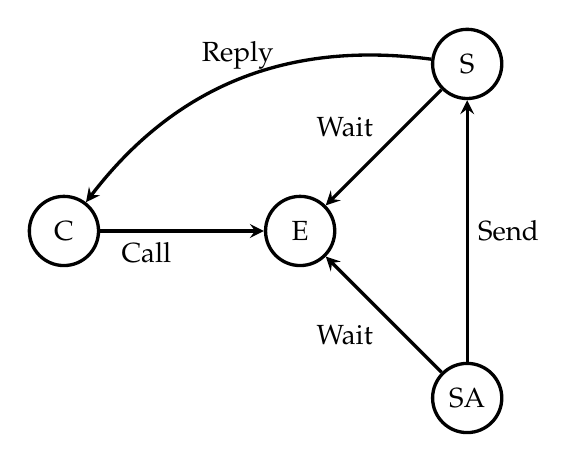
\begin{tikzpicture}[node distance=3cm,on grid,>=stealth,very thick]
        \node[state] (client)                     {C};
        \node[state] (endpoint) [right=of client] {E};
        \node[state] (server) [above right=of endpoint] {S};
        \node[state] (stack) [below right=of endpoint] {SA};

        \path[->]
            (client) edge node [below left] {Call} (endpoint)
            (server) edge node [above left] {Wait} (endpoint)
            (server) edge [bend right] node [above] {Reply} (client)
            (stack)  edge              node [below left]       {Wait} (endpoint)
            (stack)  edge              node [right] {Send} (server)
       ;
    \end{tikzpicture}
    \caption{Migrating threads with a stack allocating thread, SA.}
    \label{fig:migrating-threads}
\end{figure}

User-level systems can build multi-threaded servers with migrating threads in the following way: server threads run at priority $p$ and wait on the server endpoint.
An additional thread runs at priority $p - 1$, whose purpose is to allocate stacks.
If a client request comes in and no server thread is available to serve it, then the stack allocating thread will run, allocate a new stack and start a new server thread.
The stack allocator will forward the clients scheduling context and request onto the new server thread, and wait on the endpoint again, using the new system call \sendwait.
This is illustrated in \Cref{fig:migrating-threads} -- SA is the stack allocator, which creates server thread S after client C makes the first request.

Because the endpoint always has a thread waiting for messages (the stack allocator), the helping mechanism will not be triggered.
This scenario relies on priority ordered \gls{IPC}, and the correct ceiling priorities assigned to servers.

\subsubsection{Exception}

Temporal faults allow the user to implement custom handling for budget expiry.
A temporal fault endpoint for budget expiry is set per thread, so a server can set up a dedicated thread to wait for temporal faults.
The dedicated thread must be assigned its own reservation for handling faults.
The thread can be used to complete the request (as an emergency reservation), to rollback the request and return an error from the server, or for other purposes.
Of course, servers then must be thread safe such that the fault handling thread does not corrupt state.

\subsubsection{Bandwidth inheritance}

Bandwidth inheritance will occur if no temporal fault endpoint is registered and a blocked server encounters contention.
This allows user systems to have temporally contained servers without the requirement that those servers be thread safe.

\subsection{Summary}

This section has outlined the details of integrating resource kernel concepts of enforcement, admission and scheduling into \selfour.
We also outlined our approach to resource sharing, using scheduling context donation over IPC, and showed how this supports servers using reservation-per-thread, migrating-threads, temporal exceptions or bandwidth inheritance.

The status of the implementation so far is as follows:

\subsubsection{Implemented}

\begin{itemize}
\item Scheduling contexts.
\item EDF scheduling.
\item User-level admission control.
\item Fast-path changes.
\item Task completion when a thread waits on its bound asynchronous endpoint.
\item Temporal isolation for fixed-priority threads.
\item Scheduling context donation.
\item Converted kernel to tickless.
\end{itemize}

\subsubsection{To be implemented}

\begin{itemize}
\item \sendwait
\item Ordered \gls{IPC} endpoint queues.
\item Temporal exceptions.
\item Helping.
\item Nested Helping.
\end{itemize}



\chapter{Evaluation}
\label{chap:evaluation}

We now evaluate our model through a series of microbenchmarks, system benchmarks and case studies on
a both and ARM and x86 hardware.
First, we present the hardware platforms used in addition to the cost of timer operations on those
platforms. Then we demonstrate the minimal performance overhead of our mechanisms using a set of 
microbenchmarks which measure the overheads of the MCS kernel versus the existing \selfour kernel, 
which is referred to as \emph{baseline}.  

We then run a several system benchmarks, first comparing a Redis~\citep{redis:url} 
implementation to baseline \selfour, Linux and NetBSD to show that our kernel is competitive.
We then demonstrate temporal
isolation between threads sharing the same CPU in two scenarios,
using Redis again, followed by ipbench~\citep{Wienand_Macpherson_04}. Finally, we show isolation in a
shared encryption server, and measure the cost of various timeout fault handling policies. 

In addition, we evaluate two user-level scheduler implementations: one which implements a static
criticality switch, and a user-level \gls{EDF} implementation which we show is
competitive with an in-kernel \gls{EDF} scheduling from \litmus. Lastly, we use an \gls{IPC}
throughput benchmark to demonstrate minimal, multicore scalability overhead, and we show 
how resource server threads can migrate between processing cores.

\section{Hardware}

% describe benchmark setup, details of each hardware platform
We ran microbenchmarks on a variety of hardware to show the overheads of the model compared to
baseline \selfour. \Cref{t:evaluation-hardware} summarises the hardware platforms. \textsc{Sabre} is
the verified platform for \selfour, although at the time of writing verification for \textsc{x64} is
ongoing. Currently, the only platforms that support more than one core are \textsc{Sabre},
and \textsc{x64}.

Two of our platforms, \textsc{x64} and \textsc{Hikey} support both 32- and 64-bit execution modes.
We use both, referring to them as \textsc{ia32} and \textsc{Hikey32} when in 32-bit mode and
\textsc{x64} and \textsc{Hikey64} otherwise. All platforms have out-of-order execution, except
\textsc{Hikey}, which is in-order.

Additionally, we use several load generators running Linux on an isolated network for 
benchmarks that require a network.

\begin{table}[t]
\begin{tabularx}{\textwidth}{Xlrrrrr}\toprule
    \emph{Platform}       & \emph{Microarch.} & \emph{Clock } & L1 & L2 & L3  & TLB  \\
    \emph{Arch}           & \emph{CPU}        & GHz           & (KiB) & (KiB) & (MiB) & (entries) \\\midrule
    \textsc{KZM} (32-bit) & ARM1136JF-S       & 1.0           & 16+16       & 128      & \no      & 32\\
    \small{ARMv6}                 & i.MX31            &               & 4$\times$        & 8$\times$         & \no      & 2$\times$  \\
    \rowcolor{gray!25}
    \textsc{Sabre} (32-bit) & Cortex-A9       & 1.0           & 32+32    & 1024     & \no      & 64\\
    \rowcolor{gray!25}
    \small{ARMv7}                    & i.MX6             &               & 4$\times$  & 16 $\times$  & \no & 2$\times$  \\
    \textsc{Hikey} (64-bit)  & Cortex-A53        & 1.2           & 32+32     & 512 & \no & 128         \\
    \small{ARMv8}                    & Kirin 620         &               & 4+2$\times$       & 16$\times$    & \no   & 4$\times$  \\
    \rowcolor{gray!25}
    \textsc{TX1}   (64-bit)  & Cortex-A57        & 1.9           &  32+48 & 2,048 & \no & 256          \\
    \rowcolor{gray!25}
    \small{ARMv8}                   & Jetson TX1  &                   & 2+3$\times$       & 16$\times$ & \no & 4$\times$ \\
    \textsc{x64}    (64-bit) & i7-4770           & 3.1           & 32+32 & 256 & 8 & 128,8 \\          
    \small{x86}                     & Haswell            &                 & 8$\times$ & 8$\times$ & 16$\times$ & 8$\times$ \\
    \bottomrule
\end{tabularx}
\caption[Hardware platform details.]{Hardware platform details, ``$\times$`` is associativity, and + indicates i-cache+d-cache.}
\label{t:evaluation-hardware}
\end{table}

\section{Overheads}

We first present a suite of microbenchmarks to evaluate any performance overheads against baseline
\selfour.
For each benchmark we ensure \gls{FPU} context switching is off by performing the required number of 
system calls 
without activating it such that the kernel will cease switching the FPU context. We present
overheads on IPC operations, signalling and interrupts, and finally scheduling. 

For each of the benchmarks in this section, we measure the cost of measurement, which is reading the
cycle counter on ARM platforms, and the \gls{TSC} on x86, and subtract the value obtained
from the final result.

\subsection{Timer}
\label{s:eval-timer}

Two of the main sources of overhead introduced by our model are related to the need to read and
reprogram the timer on non-fastpath kernel entries, and when performing a scheduling context switch.
We show the results of microbenchmarks of both of these operations in \Cref{t:evaluation-timer}, and
note the timer hardware used on the specific platform. 

\begin{table}[t]\centering
\rowcolors{2}{gray!25}{white}
\begin{tabularx}{\textwidth}{lXccc}\toprule
    \emph{Platform} & \emph{Timer} & \emph{Read time} & \emph{Set timeout} & \emph{Sum}
    \\\midrule
    \textsc{KZM}               & General purpose timer    & 83 (0)   & 203(0)  & 286   \\
    \textsc{Sabre}             & ARM MPCore global timer  & 23 (0)   & 36 (0)  & 59    \\
    \textsc{Hikey32/64}        & ARM generic timers       &  6 (0)   &  6 (0)  & 12    \\
    \textsc{TX1}               & ARM generic timers       &  8 (0)   &  1 (0)  & 9     \\
    \textsc{ia32}              & TSC deadline mode        & 12 (2.2) & 220 (1.0) & 232 \\
    \textsc{x64}               & TSC deadline mode        & 11 (2.3) & 217 (2.0) & 228 \\
    \bottomrule\hline
\end{tabularx}
\caption[Latency of timer operations.]{Latency of timer operations per platform in cycles. Standard deviations shown
in parentheses.}
\label{t:evaluation-timer}
\end{table}

For both microbenchmarks, we read the timestamp before and after the operation, and do this 102
times, discarding the first two results to prime the cache.  We take the difference of the cycle
counts, and subtract the cost of measuring the cycle counter itself. The results show the cost of
both operations separately, and then their sum, which is the total measured overhead introduced by timers on
scheduling context switch.

All platforms excluding \textsc{KZM} have a 64-bit timer available, making \textsc{KZM} the only
platform requiring timer overflow interrupts, which are not measured as \textsc{KZM} is a deprecated
platform provided for comparison with modern ARM versions.

\textsc{KZM} and \textsc{Sabre} both use memory mapped timers, the 32-bit general purpose timer for
the former and 64-bit ARM global timer for the latter. \textsc{Sabre} has four cores and the timer
registers are banked, making access fast for each core. Timer access on \textsc{Sabre} is
significantly faster than the \textsc{KZM}. 

For all other ARM platforms, the ARM generic timers are available, which are accessed via the
coprocessor. The majority of new ARM platforms support the ARM generic timers. 

On \textsc{x64} we use the \gls{TSC} with \gls{TSC}-deadline
mode~\citep{Intel_64_IA-32:asdmspg_325384}, an architectural \gls{MSR} available since
Intel SandyBridge by which a local-APIC timer interrupt is triggered when the \gls{TSC} matches the
programmed value. 

\Cref{t:evaluation-timer} shows the instruction latency of each timer operation. In practice, especially
for \textsc{x64}, these operations are subject to pipeline parallelism and out-of-order execution, which
reduces the overhead.

Results on both architectures show that the overhead of a tickless kernel, which requires the timers
to be frequently read and reprogrammed, is practical on modern hardware. On ARM, timer costs have
reduced by an order of magnitude from ARMv6 through to ARMv8. 

\subsection{IPC performance}

\Gls{IPC} performance is a critical measure of the practicality and efficiency of a
microkernel~\citep{Liedtke_95}. We benchmark our \gls{IPC} operations against base system, \selfour,
which has an established efficient \gls{IPC} fastpath~\citep{Elphinstone_Heiser_13}. 

\subsubsection{Fastpath}

To evaluate IPC fastpath performance we set up a client (the caller) and server (the callee) in different
address spaces. We take timestamps on either side of the IPC operation being benchmarked and record
the difference. This is done 16 times for each result value to prime the cache, then record the next
value. Results presented are for performing this a total of 16 times. Additionally, we measure the
overhead of system calls stubs in the same way and subtract this from the measurement, to obtain
only the kernel cost of the operation\footnote{The \gls{IPC} benchmarks already existed for
 \selfour, but we modified them to support the \gls{MCS} kernel as part of this thesis}.
   The message sent is zero length, so neither the caller nor callee's \gls{IPC} buffer accessed.

\begin{table}[t]\centering
\begin{tabular}{ll r@{~}l r@{~}l r@{~}r}\toprule
\emph{Platform}           & \multicolumn{1}{c}{\emph{Operation}}
                                & \multicolumn{2}{c}{\emph{Baseline}}
                                & \multicolumn{2}{c}{\emph{MCS     }}
                                & \multicolumn{2}{c}{\emph{Overhead}} \\
    \ipcmicro{KZM}{kzm}{fastpath}
    \ipcmicro{Sabre}{sabre}{fastpath}
    \ipcmicro{Hikey32}{hikey32}{fastpath}
    \ipcmicro{Hikey64}{hikey64}{fastpath}
    \ipcmicro{TX1}{tx1}{fastpath}
    \ipcmicro{x64}{haswell}{fastpath}
    \ipcmicro{ia32}{ia32}{fastpath}
    \bottomrule
\end{tabular}
\caption[Fastpath IPC overhead]{Time in cycles for \selfour fastpath \gls{IPC}. Standard deviations shown in brackets.}
\label{t:fastpath-ipc-micro}
\end{table}

As discussed in \cref{p:impl-fastpath}, timer operations are avoided on the fastpath. However, we do
add significantly to the \call fastpath, by accessing two further objects (the scheduling context
and resume object) and two validation checks. In detail, the \call fastpath is altered as follows:

\begin{itemize}
\item We remove the reply capability lookup, so the sending \gls{TCB}'s \code{cnode} is no
        longer accessed. 
\item We read the resume object pointer from the thread state, however the thread state is already accessed
    by the \call fastpath. 
\item We check that the resume object is valid. 
\item We read from and write to the resume object to push it onto the call stack.
\item We check the destination \gls{TCB} is passive.
\item We write scheduling context that is lent over the \call to link it to the receiver, and update
    the back pointer to the resume object.
\end{itemize}

\cref{t:fastpath-ipc-micro} shows the results.
Overheads on the \call fastpath are low, with the worst effected platform being
\textsc{KZM} with a 10\% overhead, which is the oldest platform with the smallest caches. On call,
\textsc{KZM} shows L1 data cache miss and 1 memory access, which shows that the new fastpath does not
fit into the small, 16KiB L1 cache. \textsc{Sabre} suffers a 7\% overhead, due to a \gls{TLB} miss likely
due to the relatively low associativity on Cortex-A9 \glspl{TLB}.  In general, as hardware becomes newer the
overhead reduces, with the exception of the \textsc{Hikey} which is the only platform we use that has in
order execution. Additionally \textsc{Hikey} has a smaller L2 cache than the older \textsc{Sabre},
but a larger \gls{TLB} wit higher associativity.
We posit that for the Hikey, further hand optimisation of the fastpath would result in better
performance. The newest ARM hardware is the TX1, which only shows a 5\% overhead. x86 with its large
caches and highly optimised pipeline only incurs a 1\% overhead. For further detail on the
numbers read from the performance counters cited here, please see
\cref{appendix:fastpath-performance}.

The fastpath for \replyrecv has a higher impact, for two reasons: first, we add a new capability
lookup, being the resume object provided to receive, which must be looked up by the \replyrecv
fastpath. Although we remove of reply capability from the \gls{TCB}
\code{cnode}, that \code{cnode} is still accessed to validate the caller's root cspace capability
and top-level page directory capability, so that cache line is still read. Additionally, because
\gls{IPC} is now ordered, the fastpath must check if the callee's \gls{TCB} will be appended to the
endpoint queue. Otherwise, the fastpath is aborted for an ordered insert. 

As a result, the overheads shown in \cref{t:fastpath-ipc-micro} for \replyrecv are generally higher
than \call, except for \textsc{Sabre}, which already suffered some \gls{TLB} misses on
the baseline kernel, again due to low \gls{TLB} associativity.

\subsubsection{Slowpath}
\label{eval:slowpath}

Now we evaluate the \gls{IPC} slowpath, for both active and passive threads. Unlike the fastpath, the slowpath
generally doesn't fit into the cache and shows erratic results with high standard deviations on our
hardware, slowpath benchmarks are conducted differently. For the slowpath benchmarks, we set up a
pair of threads to do \call and \replyrecv 10,000 times and divide the result by 10,000. We do this
for 110 runs, abandoning the first 10, to calculate the standard deviation and average. In order to guarantee that we hit the
slowpath on a non-error condition, we set the message length to ten words. 

\cref{t:slowpath-ipc-micro} shows the results for round-trip, slowpath \gls{IPC}. For passive, slowpath IPC
we see the cost of the
timer read, extra objects and extra code. The overhead decreases as hardware caches increase in size and
timer accesses faster (for ARM the worst result is on the \textsc{KZM} and best on \textsc{TX1}).
For active slowpath \gls{IPC}, the scheduling context is changed on the IPC, invoking the sporadic
check routines and requiring a time reprogram. 

It should be noted that the slowpath is avoided in most cases, as long IPC is discouraged in
favour of establishing shared memory protocols to transfer large amounts of data. The majority of
fastpath checks make sure the thread being switched to is valid and runnable. Only two cases hit the
fastpath frequently: if a medium priority thread has woken, and is higher priority than the
\gls{IPC} target, and if the target is active, not passive. 
Additionally, many improvements can be made to the \gls{IPC} slowpath to improve
performance, but it has not been examined extensively.

\begin{table}[hb]\centering
\begin{tabular}{ll r@{~}l r@{~}l r@{~}r}\toprule
\emph{Platform}           & \multicolumn{1}{c}{\emph{Operation}}
                                & \multicolumn{2}{c}{\emph{Base}}
                                & \multicolumn{2}{c}{\emph{MCS}}
                                & \multicolumn{2}{c}{\emph{Overhead}}\\
    \ipcmicro{KZM}{kzm}{slowpath}
    \ipcmicro{Sabre}{sabre}{slowpath}
    \ipcmicro{Hikey32}{hikey32}{slowpath}
    \ipcmicro{Hikey64}{hikey64}{slowpath}
    \ipcmicro{TX1}{tx1}{slowpath}
    \ipcmicro{x64}{haswell}{slowpath}
    \ipcmicro{ia32}{ia32}{slowpath}
    \bottomrule
\end{tabular}
\caption[Slowpath IPC overhead.]{Slowpath IPC overhead in cycles, baseline \selfour versus MCS.
Standard deviations shown in brackets.} \label{t:slowpath-ipc-micro}
\end{table}

\subsection{Faults}

Recall that fault handling in \selfour occurs via an \gls{IPC} simulated by the kernel to a fault
endpoint, which a fault handling thread blocks on, waiting for any fault messages (\cref{api:faults}). 

To measure the fault handling cost, we run two threads in the same address space: a fault handler
and a faulting thread, with the same priority. We trigger a fault by executing an undefined instruction in a loop on the faulting thread's
side. The fault handler then increments the instruction pointer past the undefined
instruction, and the benchmark continues.  As this is also a slowpath we use the same method as
above, and measure the amount of time it takes for 10,000 faults then divide the result. We do this
for 110 runs, abandoning the first 10, to calculate the standard deviation and average. 

We measure both active and passive fault handling, and the results, shown in
\cref{t:slowpath-fault-micro}, are similar to slowpath
\gls{IPC}, being slower for active, and improving as cache-size and timer operation cost reduces. 
Note that although there is currently no fastpath for fault handling, it is merely a matter of
engineering effort to add one should this become a performance issue. 

We do not show results for the \textsc{KZM} platform, as it is ARMv6 and the performance monitor
unit, including the cycle counter, cannot be read from user mode. Further, the use the undefined instruction 
to read the cycle counter efficiently on this platform, so the fault benchmark does not work.

\begin{table}[t]\centering
\begin{tabular}{cl r@{~}l  r@{~}l r@{~}r}\toprule
\emph{Platform}           & \multicolumn{1}{c}{\emph{Operation}}
                                & \multicolumn{2}{c}{\emph{Baseline}}
                                & \multicolumn{2}{c}{\emph{MCS}}
                                & \multicolumn{2}{c}{\emph{Overhead}} \\ 
    % no kzm, fault benchmark doesn't work
    \faultmicro{Sabre}{sabre}
    \faultmicro{Hikey32}{hikey32}
    \faultmicro{Hikey64}{hikey64}
    \faultmicro{TX1}{tx1}
    \faultmicro{x64}{haswell}
    \faultmicro{ia32}{ia32}
    \bottomrule
\end{tabular}
\caption[Fault handler overhead.]{Fault IPC slowpath overhead in cycles, baseline \selfour versus
MCS. Standard deviations shown in brackets.}
\label{t:slowpath-fault-micro}
\end{table}

\subsection{Signalling and interrupts}

As noted in the previous section, mainly engineering effort is required to add new fastpaths. For
this reason, we add two new (non-verified) experimental fastpaths to the kernel: one for interrupt
delivery, and the other for signalling a low-priority thread, which we now examine.

We measure interrupt latency using two threads, one spinning in a loop
updating a volatile cycle counter, the other, higher priority thread
waiting for an interrupt. On delivery, the handler thread determines the
interrupt latency by subtracting the
looped timestamp from the current time. The overhead is higher here as we must switch scheduling
contexts, which requires reprogramming the timer, however the scheduler is by-passed as the switch
is to a higher priority thread. \textsc{KZM} shows the  highest overhead, where once again we
exceed the small cache. The \textsc{Hikey} pays for its in order execution pipeline, which could be
improved with further profiling of the fastpath. The \textsc{TX1} shows the least impact, with only
a 5\% increase on the interrupt fastpath, as shown in \cref{t:micro-irq}. 

\code{signal()}, on the other hand shows little overhead as it does not alter the
scheduling context or access to the timer device.  In this benchmark, a high priority thread signals
a low priority thread, a common operation for interrupt service routines. As \cref{t:micro-irq}
shows, in 
cases where slowpath performance is a issue, further fastpaths can be added to avoid accessing the
timer, in the case where older hardware is required.

\begin{table}[t]\centering
\begin{tabular}{cl r@{~}l r@{~}l r@{~}r}\toprule
\emph{Platform}           & \multicolumn{1}{c}{\emph{Operation}}
                                & \multicolumn{2}{c}{\emph{Base}}
                                & \multicolumn{2}{c}{\emph{MCS}}
                                & \multicolumn{2}{c}{\emph{Overhead}} \\
    \irqmicro{KZM}{kzm}
    \irqmicro{Sabre}{sabre}
    \irqmicro{Hikey32}{hikey32}
    \irqmicro{Hikey64}{hikey64}
    \irqmicro{TX1}{tx1}
    \irqmicro{x64}{haswell}
    \irqmicro{ia32}{ia32}
    \bottomrule
\end{tabular}
\caption[Fastpath IRQ and Signal overhead.]{Fastpath IRQ and signal overhead in cycles, baseline
    \selfour versus MCS. Standard deviations shown in brackets.}
\label{t:micro-irq}
\end{table}

\subsection{Scheduling}

\begin{table}[t]\centering
\begin{tabular}{cl r@{~}l  r@{~}l r@{~}r}\toprule
\emph{Platform}           & \multicolumn{1}{c}{\emph{Operation}}
                                & \multicolumn{2}{c}{\emph{Base}}
                                & \multicolumn{2}{c}{\emph{MCS}}
                                & \multicolumn{2}{c}{\emph{Overhead}} \\

    
    \schedulemicro{KZM}{kzm}
    \schedulemicro{Sabre}{sabre}
    \schedulemicro{Hikey32}{hikey32}
    \schedulemicro{Hikey64}{hikey64}
    \schedulemicro{TX1}{tx1}
    \schedulemicro{x64}{haswell}
    \schedulemicro{ia32}{ia32}
    \bottomrule
\end{tabular}
\caption[Slowpath yield and scheduler costs.]{Slowpath yield and scheduler costs in cycles, baseline \selfour 
versus MCS. Standard deviations shown in brackets.}
\label{t:micro-schedule}
\end{table}

In our final microbenchmark we look at the cost of the scheduler, and the \yield system call. 

The \code{schedule} benchmark measures the cost of a signal to a higher priority thread, which forces 
a reschedule operation and does not avoid picking a new thread from the scheduler, in addition to
all other slowpath overheads. Like the other slowpath benchmarks, we take the average of 10,000
runs. 
The scheduler is by definition a slowpath activity, as it is completely avoided on the fastpath, and
much of the slowpath, by the lazy scheduling mechanism (\cref{sec:sel4-scheduler-opt}).
\cref{t:micro-schedule} shows that scheduling cost increases noticeably, however note that \selfour IPC,
particularly scheduler-context donation (and its predecessor, the
undisciplined timeslice donation), is designed to minimise the need for
invoking the scheduler, therefore this increase is unlikely to have
a noticeable effect in practice. 

We also measure the average cost for the current thread to \yield to itself. This is not so much an
overhead as a completely different system call: previously \yield was incomplete, and would simply
dequeue and enqueue the current thread from the scheduling queues, before returning to user level.
\yield in the new model charges the remaining budget in the head replenishment to the thread, and
triggers a timer reprogram. Although semantically similar for round robin threads, \yield does a lot
more, hence the drastic overheads shown in \cref{t:micro-schedule}.

\subsection{Full system benchmark}
\label{s:evaluation-redis-overhead}

To demonstrate the impact of the overheads in a real system scenario, 
we measure the performance of the Redis key value store~\citep{redis:url} using 
\gls{YCSB}~\citep{Cooper_STRS_10} on baseline and MCS \selfour, and compare this
against Linux, the Rump unikernel~\citep{Kantee_Cormack_14} and 
NetBSD~\citep{NetBSD:url} all on the \textsc{x64} machine.

For \selfour, we use a single-core Rump library OS~\citep{Kantee_Cormack_14} to provide 
NetBSD~\citep{NetBSD:url} network drivers at user level, by leveraging an existing port of this infrastructure
to \selfour~\citep{McCleod:be}.
The system consists of Redis/Rump running on three active \selfour threads: 
two for servicing interrupts (network, timer) and one for Rump, as shown in
\cref{f:redis-arch}. Interrupt threads run at the highest priority,
followed by Redis and a low-priority idle thread (not shown) for measuring CPU utilisation;
this setup forces frequent invocations of the scheduler and interrupt path.

 \begin{figure}[ht]
    \centering
    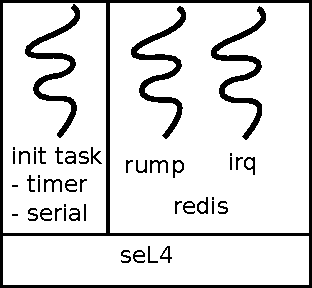
\includegraphics{redis-arch}
    \caption[System architecture of Redis benchmark.]{System architecture of the Redis / \gls{YCSB} benchmark on \selfour, 
        Linux, NetBSD and Rump unikernel.}
    \label{f:redis-arch}
\end{figure}

\cref{t:redis} shows the achieved throughput of Redis+Rump
running \gls{BMK}, and Redis on the seL4 baseline and as well as the MCS
branch, plus Linux and NetBSD (7.0.2) for comparison. \cref{f:redis-arch} shows the \selfour set up,
compared with the architecture of Redis on Linux, NetBSD and \gls{BMK}. 

\cref{t:redis} indicates the interrupt handling method used, as there is no single method supported
across all four scenarios. \gls{BMK} only supports the legacy
\gls{PIC},
while NetBSD only supports \glspl{MSI}. Linux and seL4 both support the
advanced \gls{APIC}.

The utilisation figures show that the system is fully loaded, except
in the Linux case, where there is a small amount of idle time. The
cost per operation (utilisation over throughput) is best on Linux, a
result of its highly optimised drivers and network stack. Our
bare-metal and \selfour-based setups use Rump's NetBSD drivers, and
actually performance within a few percent of native NetBSD. This
indicates that the MCS model comes with low overhead.

\begin{table}[t]\centering
      \rowcolors{3}{}{gray!25}
      \begin{tabularx}{\textwidth}{Xrrrrr}\toprule
          \emph{System}   & \emph{IRQ} & \emph{Throughput} & \emph{Utilisation} & \emph{Cost} & \emph{Latency} \\
                          &            & (k ops/s)         & (\%)               & per op.     & (ms)            \\
        \midrule

      \input{data/ycsb-redis.inc}
      \bottomrule
    \end{tabularx}
    \caption[Results of Redis throughput benchmark.]{Throughput (k\,ops/s) achieved by Redis using the YCSB
      workload A with 2 clients.  Latency is the average Read and Update,
      standard deviations in parentheses and omitted where less than the least
      significant digit shown.}
    \label{t:redis}
\end{table}

\section{Temporal Isolation}

We have demonstrated our model has little overhead and is competitive with existing monolithic
kernels. Now we evaluate temporal isolation properties, between processes and in a shared-server
scenario. 
In addition, we evaluate and demonstrate different
techniques to restore server state after a timeout exception.

% Show isolation between processes using different scheduling contexts
\subsection{Process isolation} 

We evaluate process isolation, where processes do not share resources, indirectly via network
throughput and network latency in two separate benchmarks. Note that the Rump unikernel only
currently supports x86 platforms, consequently these experiments are only carried out on
the \textsc{x64} platform. 

\subsubsection{Network throughput}

First, we demonstrate our isolation properties with the Redis architecture described in
\Cref{s:evaluation-redis-overhead} with an additional, high-priority active CPU-hog thread
competing for \gls{CPU} time.  All scheduling contexts in the system are configured with a
5\,ms period. We use the budget of the CPU-hog to control the amount of time left over
for the server configuration. \autoref{f:redis} shows the throughput
achieved by the YCSB-A workload as a function of the available CPU
bandwidth (i.e \ the complement of the bandwidth granted to the CPU-hog
thread). All data points are the average of three benchmark runs.

\begin{figure}[h]
  \centering
  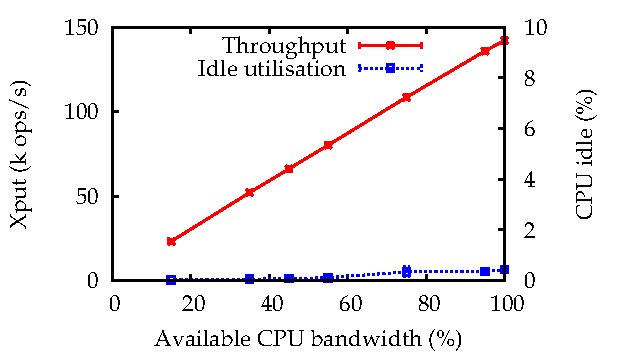
\includegraphics{redis}
  \caption[Results of Redis isolation benchmark.]{Throughput of Redis YCSB workload A and idle time versus available bandwidth.}
  \label{f:redis}
\end{figure}

The graph shows that the server is CPU limited (as indicated by very low idle time)
and consequently throughput scales linearly with available CPU
bandwidth.

\subsubsection{Network latency}

Second, we evaluate process isolation via network latency in a system shown in \cref{f:ipbench-arch}. 
The system consists of a single-core of a Linux \gls{VM} which runs at a high priority with a
constrained budget and a \gls{UDP} echo server running at a lower priority,
representing a lower-rate \textsc{high} thread. We
measure the average  and maximum UDP latency reported by the
ipbench~\citep{Wienand_Macpherson_04} latency test.

\begin{figure}[h]
    \centering
    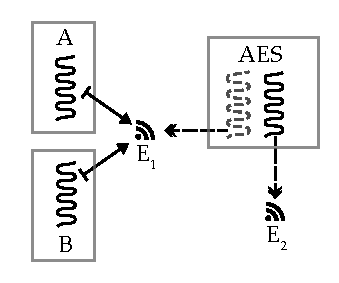
\includegraphics{ipbench-arch}
    \caption{System architecture of ipbench benchmark.}
    \label{f:ipbench-arch}
\end{figure}


Specifically, the Linux VM interacts with timer (PIT) and serial device drivers implemented as
passive servers outside the \gls{VM}; all three components are at a high priority. In the Linux server we
run a program (\code{yes > /dev/null}) which consumes all available
CPU bandwidth.  The UDP echo server, completely isolated from the Linux instance during the
benchmark, but sharing the
serial driver, runs at a low priority with its own HPET timer
driver.

Two client machines run ipbench daemons to send packets to the UDP-echo server on the target machine
(\textsc{x64}). The control machine, one of the load generators, runs ipbench with a \gls{UDP} socket at 10\,Mbps over a 1\,Gb/s Ethernet connection with 100-byte packets. The Linux VM has a 10\,ms period and we vary the
budget between 1\,ms and 9\,ms.
We represent the zero-budget case by an unconstrained Linux that is not running any user code.
Any time not consumed by Linux is available to UDP echo for processing
10,000 packets per second, or 100 packets in the time left over from
each of Linux's 10\,ms period.

\autoref{f:ipbench} shows the average and maximum \gls{UDP} latencies for
ten runs at each budget setting. We can see that the maximum latencies
follow exactly the budget of the Linux server (black line) up to 9\,ms. Only
when Linux has a full budget (10\,ms), and thus able to monopolise the
processor, does the UDP server miss its deadlines, resulting in a
latency spike.  This result shows that our sporadic server implementation is effective in bounding
interference of a high-priority process.

\begin{figure}[h]
  \centering
  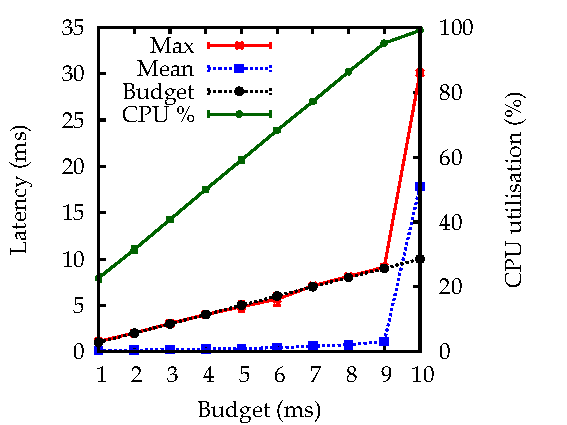
\includegraphics{ipbench}
  \caption[Results of ipbench isolation benchmark.]{Average and maximum latency of UDP packets with
  a CPU-hog VM running a high priority with a 10\,ms budget.}
  \label{f:ipbench}
\end{figure}

% Show isolation in a shared server
\subsection{Server isolation} 
\label{s:server-isolation}

To demonstrate temporal isolation in a shared server, we use a case study of an encryption service
using \gls{AES} to encrypt client data. We measure both the overhead of different
recovery techniques, and the throughput achieved when two clients constantly run out of budget in the server. 
We port an existing, open-source \gls{AES} implementation to a shared server running on \selfour, and run
benchmarks on both \textsc{x86} and \textsc{Sabre}.

\Cref{f:aes-arch} shows the architecture of the case study. Both clients $A$ and $B$ are single
 threaded and exist in separate address spaces to the server. The server has two threads, a passive
 thread for serving request on the clients scheduling context and an active thread which handles
 timeout exceptions for the server. The server and timeout exception handler share the same virtual
 memory and capability spaces.

\begin{figure}
\centering
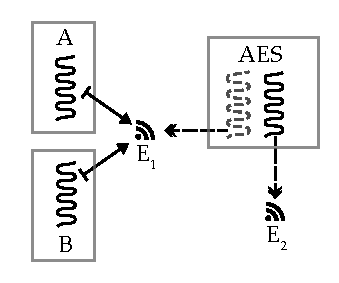
\includegraphics{aes-arch}
\caption[Architecture of the AES case study.]{Architecture of the \gls{AES} case study. Client $A$ and $B$ make \gls{IPC} requests over
endpoint $E_{1}$ of passive $AES$ which has an active timeout fault handling thread waiting for
fault \gls{IPC} messages on endpoint $E_{2}$.}
\label{f:aes-arch}
\end{figure}

The server itself runs the AES-256 algorithm with a block size of 16~bytes. The server alternates between two
buffers, using an atomic swap, of which one always contains consistent state, the other is
dirty during processing. When a timeout fault occurs, only the dirty buffer is lost due to
inconsistency. Both clients request 4\,MiB of data to be encrypted, and have a budget insufficient to
complete the request. When the server is running on the clients scheduling context and the budget
expires, a timeout exception, which is a fault IPC message from the kernel, is delivered to the timeout
handler. 

\subsection{Timeout handling techniques}

If client scheduling context is depleted while the server is servicing the request, a timeout fault
is raised and sent to the timeout handler.  The appropriate protocol for handling such faults
depends ultimately on the requirements of the system.  Consequently, we implement and evaluate four
different timeout fault handling techniques: rollback, error, emergency and extend. 

While each technique is evaluated separately, combinations of such techniques could be used for
different clients depending on their requirements. For example, trusted clients may get special
treatment. Note that in all cases of blocking IPC, clients must trust the server as discussed in
\cref{s:locking}. Additionally, although out experiment places 
the timeout fault handler in the server's address
space, this is not necessary: for approaches that require access to scheduling contexts and
scheduling control capabilities, the timeout handler may be placed in a scheduling servers address
space, separate from the server itself.

\subsubsection{Rollback}

Rollback restores the server to the last known consistent state recorded. In the case of non-thread
safe servers, this may require rolling back an entire request. However, algorithms like \gls{AES}
which can easily be batched can make progress. The process for rollback involves is as follows:

\begin{enumerate}\label{e:rollback}
    \item A timeout fault is received by timeout handler, $T$ over $E_{2}$.
    \item $T$ constructs a reply message to the client from the last clean state, and sends this 
        message to the client by invoking the resume capability that the server has used for that client. 
        Because the resume object tracks the donation, the client's scheduling context is returned.
    \item $T$ then restores the server, $S$ to a known state by the timeout handler (restoring registers,
        stack frames and any global state). $S$ is restored to the point before it made its
        last system call, usually an \nbsendrecv, which it used to indicate to the initialiser that
        $S$ should be made passive, as part of the passive server initialisation protocol presented
        in \cref{sec:impl-passive-servers}.
    \item Now the server must return to blocking on the IPC endpoint, $E_{1}$. $T$ binds a
        scheduling context to $S$ and waits for a message. 
    \item Now the $S$ runs from its checkpoint, repeating the \nbsendrecv, signalling to $T$ that it
        can now be converted to passive once more and blocking on $E_{1}$. 
    \item $T$ wakes and converts the server back to passive.
    \item Finally, $T$ blocks on $E_{2}$, ready for further timeout faults.
\end{enumerate}

The rollback technique requires the server and timeout handler to both have access to the reply
object that the server is using, and the servers \gls{TCB}, meaning the timeout handler must be
trusted by the server. In our example the server and timeout handler run at the same priority, in
all cases both must run at higher priorities than the clients. 

Once the budget of the faulting client is replenished, it can then continue the request based on the
content of the reply message sent by the timeout handler. Clients are guaranteed progress as long as
their budget is sufficient to complete a single batch of progress.

If rollback is not suitable, the server can be similarly reset to the initial state and an error
returned to the client. However, this does not guarantee progress for clients with insufficient
budgets.

\subsubsection{Kill}

In cases of non-preemptible servers, potentially due to a lack of thread safety, one option is to
kill client threads. Such a scenario would stop untrusted misbehaving clients from constantly
monopolising server time.  We implement an example were the timeout handler has access to client \gls{TCB}
capabilities and simply calls suspend, however the server could also switch to a new reply object
and leave the client blocked forever, without access to any of the clients capabilities. 

The process for suspending the client is the same as that for \Cref{e:rollback} but for two aspects;
the server state does not need to be altered by the timeout handler as the server always 
restores to the same place, instead of replying to the client it is suspended.

\subsubsection{Emergency}

Another technique gives the server a one-off emergency budget to finish the client request, after
which the exception handler resets the server to being passive. This could be used in low
criticality \gls{SRT}
scenarios where isolation is desired but transient overruns are expected.
An example emergency protocol follows:

\begin{enumerate}\label{e:emergency}
    \item A timeout fault is received by timeout handler, $T$ over $E_{2}$.
    \item $T$ unbinds the client scheduling context from $S$.
    \item $T$ binds a new scheduling context to the $S$, which acts as an emergency budget.
    \item $T$ then replies to the timeout fault, resuming $S$.
    \item Now $T$ enqueues itself on $E_{1}$, such that when the server finishes the blocked request,
        $T$, being a higher priority, is served next.
    \item $S$ completes the request and replies to the client.
    \item $S$ receives the request from $T$, and replies immediate as it is an empty request.
    \item $T$ wakes, and converts the server back to passive.
    \item Finally $T$ blocks on $E_{2}$, ready for further timeout faults.
\end{enumerate}

This case requires the timeout handler to have access to client scheduling contexts in order to
unbind them from the server. 

\subsubsection{Extend}

The final technique is to simply increase the clients budget on each timeout, which requires the
timeout fault handler to have access to the clients scheduling contexts.
This could be deployed in \gls{SRT} systems or for specific threads with unknown budgets up to a limit. 

\begin{enumerate}\label{e:extend}
    \item A timeout fault is received by timeout handler, $T$ over $E_{2}$.
    \item $T$ extends the client's budget by configuring scheduling context.
    \item $T$ replies to the fault message, which resumes $S$.
\end{enumerate}

\subsection{Results}

We measure the pure handling overhead in each case, from when the timeout handler wakes up to when
it blocks again.  Given the small amount of rollback state, this measures the baseline overhead. For
schedulability analysis, the actual cost of the rollback would have to be added, in addition to the
duration of the timeout fault IPC. 
 
We run each benchmark with hot caches (primed by some warm-up
iterations)  as well as cold (flushed) caches and measure the 
latency of timeout handling, from the time the handler wakes up
until it replies to the server.

\autoref{t:rollback} shows the results. The maximum
cold-cache cost, which is relevant for schedulability analysis, differs by a factor of 3--4 between
the different recovery scenarios, indicating that all are about equally feasible.  Approaches that
restart the server and send \glspl{IPC} messages on its behalf (rollback, reply) are the most
expensive as they must restore the server state from a checkpoint and follow the passive server
initialisation protocol (recall \cref{sec:impl-passive-servers}). 

\newpage
\begin{table}[h]\centering
\begin{tabular}{cllrrrr}\toprule
\emph{Platform} & \emph{Operation} & \emph{Cache} & \emph{Min} &
                          \emph{Max} & \emph{Mean} &
                          \multicolumn{1}{c}{\boldmath \(\sigma\)} \\\midrule
                          \multirow{8}{*}{\textsc{x64}}
                          \input{data/generated/haswell-aes.inc}
                          \midrule
                          \multirow{8}{*}{\textsc{Sabre}} 
                          \input{data/generated/sabre-aes.inc} 
                          \midrule
                          \multirow{8}{*}{\textsc{Hikey64}} 
                          \input{data/generated/hikey64-aes.inc} 
                          \midrule
                          \multirow{8}{*}{\textsc{TX1}} 
                          \input{data/generated/tx1-aes.inc} 
                          \bottomrule
\end{tabular}
\caption[Cost of timeout handler operations.]{Cost of timeout handler operations in \(\mu\)s, as measured
  by timeout exception handler. \(\sigma\) is the standard deviation.}
\label{t:rollback}
\end{table}
\clearpage
\subsection{Rollback isolation}

We next demonstrate temporal isolation in the server by using the rollback
technique and measuring the time taken to encrypt 10 requests of 4\,MiB of
data. \autoref{f:aes} shows the result with both clients having the same
period, which we vary between 10\,ms and 1000\,ms.
In each graph we vary the clients' budgets between 0 and the
period. The extreme ends are special, as one of the clients has a full
budget and keeps invoking the server without ever getting rolled back,
thus monopolising the processor. In all other cases, each client
processes at most 4\,MiB of data per period, and either succeeds (if
the budget is sufficient) or is rolled back after processing less than 4\,MiB.

\begin{figure*}[t]
  \centering
  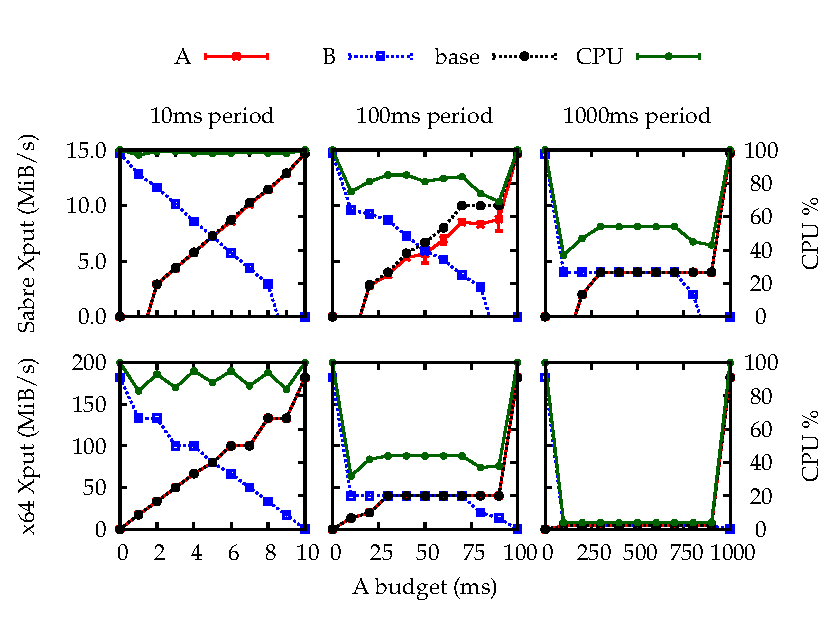
\includegraphics{aes-shared}
  \caption[Results of AES server isolation benchmark.]{Throughput for clients A and B of a passive AES server processing 10 requests of 4\,MiB of data with
      limited budgets on the \textsc{x64} (top row) and \textsc{Sabre} (bottom row) platforms. The two clients' budgets
      add up to the period, which is varied between graphs (10, 100, 1000\,ms). Clients sleep when
      they process each 4\,MiB, until the next period, except when their budgets are full. Each data point is the average of 10 runs, error bars show the standard deviation.}
  \label{f:aes}
\end{figure*}


The results show that in the CPU-limited cases (left graphs)
we have the expected near perfect proportionality between throughput and
budget (with slight wiggles due to the rollbacks), showing isolation between clients. In the cases where there is headspace (centre of the right
graphs), both clients achieve their desired throughput.

\section{Practicality}

Fundamental to the microkernel philosophy is keeping policy out of the
kernel as much as possible, and instead providing general mechanisms
that allow the implementation of arbitrary policies
\citep{Heiser_Elphinstone_16}.  As on the face of it, our
fixed-priority-based model seems to violate this principle,  we
demonstrate that the model is general enough to support the efficient
implementation of alternate policies at user level. Specifically, we
implement two user-level schedulers: first, a static mixed criticality
scheduler~\citep{Baruah_BD_11}, which we also compare to an in-kernel
implementation and secondly an \gls{EDF} scheduler, which we compare to \litmus.

\subsection{Criticality}

Static, mixed-criticality, fixed-priority schedulers are based on \emph{mode
switches}, which effectively mean altering the priority of threads in bulk:
critical threads that may be of low rate are bumped higher than their
low-criticality counter parts, to ensure deadlines are met in exceptional
circumstances. 

We implement a kernel mechanism for changing priorities in bulk of threads 
and compare with a user-level approach which simply changes the priority of threads
one at a time. In our prototype implementation, the kernel tracks all threads of specific criticalities and boosts their priority on a made switch. However, given threads are kept in per-priority queues, each thread must be removed and reinserted into a new queue, so either way the complexity of the mode-switch is $O(n)$. 

\begin{figure}
  \centering
  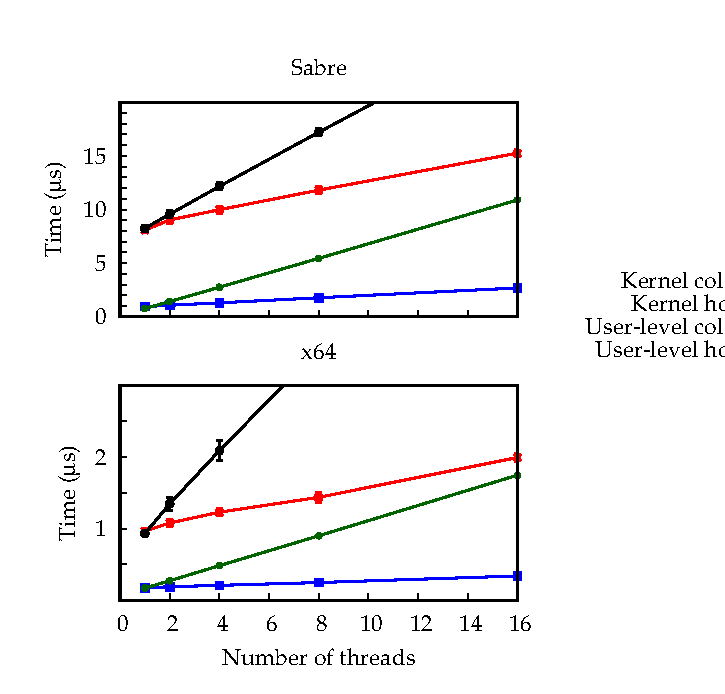
\includegraphics[width=\textwidth]{mode-switch-all}
  \caption[Kernel vs. user-level criticality switch.]{Cost of switching the priority of $n$ threads in kernel and user level, with hot
      and cold caches, on \textsc{x64} (top-left), \textsc{TX1} (top-right), \textsc{Hikey64}
      (bottom-left) and \textsc{Sabre} (bottom-right). All data points are the average of 100 runs,
                  with very small standard deviations.}
  \label{f:mode-switch}
\end{figure}

\autoref{f:mode-switch} shows the results measured with a primed cache (hot) and flushed cache (cold).
As the graph shows, switching is linear in the number of threads being boosted, in both kernel and
user-level implementations.
\Cref{t:cold-prio-switch} compares the results of cold, in-kernel switching to user-level in roughly
absolute terms. \textsc{Hikey64} is the slowest at 30\,\(\mu\)s with eight threads to switch,
due to the smaller L2 cache and
in-order execution, however all platforms show roughly the same factor of two increase when
However, most systems will not have more than a few high-criticality threads, and deadlines for critical control loops in
cyber-physical systems tend to be in the tens of milliseconds, we
conclude that criticality can be implemented at user-level, in line with standard microkernel philosophy.

The higher cost from user-level operation results from  multiple
switches between kernel and user mode, and the repeated
thread-capability look-ups. It could be significantly reduced if seL4
had a way to batch system calls, but to date we have seen no compelling use cases for this.

\begin{table}[t]\centering
    \rowcolors{2}{gray!25}{}
    \begin{tabular}{lrrr}\toprule
        \emph{Platform}     & \emph{Kernel cold ($\mu$s)} & \emph{User-level cold ($\mu$s)} & \emph{Diff $\mu$s} \\\midrule
        \textsc{x64}    & $\leq2$ & $\leq4$ & $\tilde2$ \\
        \textsc{TX1}    & $\leq4$ & $\leq8$ & $\tilde4$ \\
        \textsc{Hikey64}    & $\leq18$ & $\leq30$ & $\tilde12$ \\
        \textsc{Sabre}    & $\leq12$ & $\leq22$ & $\tilde10$ \\
        \bottomrule
\end{tabular}
\caption[Comparison of kernel and user-level priority switches]{Comparison of cold, in-kernel
priority switch to cold, user-level priority switch.}
\label{t:cold-prio-switch}
\end{table}


As a second criticality-switch benchmark, we ported three processor intensive 
benchmarks from the MiBench~\citep{Guthaus_REAMB_01} to act as workloads. 
We use \textsc{susan}, which performs image recognition, \textsc{jpeg}, which does image
encoding/decoding, and \textsc{mad}, which plays an MP3 file.
Each benchmark runs in its own Rump process
with an in-memory file system, and shares a timer and serial server.
 We chose these specific
benchmarks as they were the easiest to adapt as described below,
rather than for comparing systems, so there is no issue of bias from sub-setting.

We altered the benchmarks to run periodically in multiple stages. To obtain
execution times long enough, some benchmarks iterate a fixed number of times per
stage. Each benchmark process executes its workload and then waits for the next period to start.
Deadlines are implicit: if a periodic job finishes before the start of the next period it is
considered successful, otherwise the deadline is missed.

We run the benchmarks on both the user-level and in-kernel implementations of static mixed criticality, with 10 runs of each.

\Cref{t:modeswitch} lists the benchmarks with periods and criticalities.
\textit{susan}, the most critical, has three stages: edge detection, smoothing, and corners. The
next critical task, \textit{jpeg}, has two stages: encode, and decode. The least
critical task, \textit{mad} has only one stage. We run the benchmark
for 20\,s for each of the stages (repeating the last phase where
threads have no new phase), and
increment the system criticality level at stage transition. The parameters are arranged such that
rate-monotonic priorities are inverse to the criticalities.

\textsc{susan}, the most critical, has three stages: edge detection, smoothing, and corners. The
next critical task, \textsc{jpeg}, has two stages: encode, and decode. The least
critical task, \textsc{mad} has only one stage. We run the benchmark
for 20\,s for each of the stages (repeating the last phase where
threads have no new phase), and
increment the system criticality level at stage transition. The parameters are arranged such that rate-monotonic priorities are inverse to the criticalities.

Results are shown in \autoref{t:modeswitch}.
Only the lowest-priority thread is affected by the criticality switch, with an additional missed deadline due to
perturbations in run time due to the user-level versus kernel scheduler.
For stage one, the entire workload is schedulable and
there are no deadline misses. For stage two, the workload is not
schedulable, and the criticality switch boosts the priorities of
\textsc{susan} and \textsc{jpeg}, such that they meet
their deadlines, but
\textsc{mad} does not. In the final stage, only the most critical task
meets all deadlines.
This shows that it is sufficient to implement criticality at user-level, and our mechanisms operate as intended.

\begin{table}[h]
    \centering
    \begin{tabular}{lcccccclcl}\toprule
        \emph{Application} & \emph{T} & \emph{L} & \emph{\(L_S\)} & \emph{C} & \emph{U} & \emph{j} &
        & \emph{m}  & \\\midrule
        \input{data/generated/mode_switch.inc}
        \bottomrule
    \end{tabular}
    \caption[Results of criticality switch benchmark.]{Results of criticality switch benchmark for each
        stage, where the  criticality \(L_S\) is raised each stage. \(T\) =
        period, \textit{C} = worst observed execution time (ms),
      \textit{U} = allowed utilisation (budget/period),
      \textit{m} = deadline misses, \textit{j} = jobs completed. We recorded 52 (0.1), 86 (15.2)
      and 100 (0.0)\% CPU
utilisation for each stage respectively. Standard deviations are shown in parentheses.}
    \label{t:modeswitch}
\end{table}

\subsection{User-level EDF}\label{s:edf-impl}

We implement the EDF scheduler as an active server with active
clients which run at an \selfour priority below the user-level scheduler.
The scheduler waits on an endpoint on which it receives messages from
its clients and the timer.

Each client has a period, representing its relative deadline, and a full reservation (equal to the period). Clients
either notify the scheduler of completion by an IPC
message, or else create a timeout exception on preemption, which is also received by the
scheduler. Either is an indication that the next thread should be scheduled.

We use the \emph{randfixedsum}~\citep{Emberson_SD_10} algorithm to
generate deadlines between 10 and 1000\,ms for a certain number of threads.
A set of threads runs until 100
scheduling decisions have been recorded. We repeat this 10 times,
resulting in 1,000 scheduler runs for each data point.

We measure the scheduler latency by recording the timestamp when each client thread, and an idle
thread, detects a
context switch and processing the difference in timestamp pairs offline. We run two schedulers:
\emph{pre}-empt where threads never yield and must incur a timeout exception, and \emph{coop}, where
threads use IPC to yield to the scheduler. The latter invokes the user level timer
driver more often as the release queue is nearly always full, which involves more kernel invocations
to acknowledge the IRQ, in addition to reprogramming the timer.

We compare our latencies to those of
LITMUS$^{RT}$~\citep{Calandrino_LBDA_06}, a widely-used real-time scheduling
framework for developing real-time schedulers and locking protocols. 
As it is  embedded in Linux, LITMUS$^{RT}$ is not aimed at high-assurance systems.

We use Feather-Trace~\citep{Brandenburg_Anderson_07} to gather data.
We use the C-EDF scheduler, which is a partitioned (per-core) EDF scheduler, on a single
core. We use the same parameters and thread sets, running each set for 10\,s. 
The measured overhead considers the in-kernel scheduler, context-switch and user-level code to return to
the user.

\autoref{f:edf} shows that our preemptive user-level EDF scheduler implementation is
actually faster than the in-kernel EDF scheduler from LITMUS$^{RT}$, and
that the cost of implementing scheduling policy at user level is of
the same order as the in-kernel default scheduler. In other words,
implementing different policies on top of the base scheduler is quite feasible.

\begin{figure}[t]
    \centering
    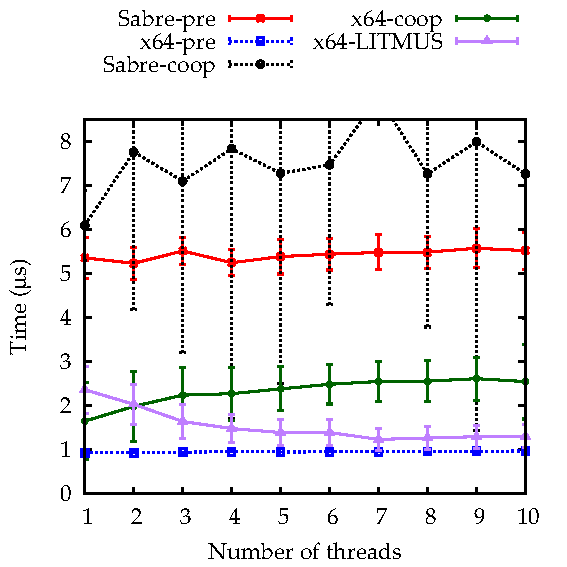
\includegraphics{edf}
    \caption[Results of \selfour user-level EDF versus \litmus.]{Execution time of \selfour user-mode EDF scheduler compared to
             kernel scheduler in \textsc{x64} \litmus.}
    \label{f:edf}
\end{figure}

\section{Multiprocessor benchmarks}

We run two multicore benchmarks, the first evaluating multicore throughput of the MCS kernel versus the
baseline kernel, the second based on our shared server \gls{AES} case study to demonstrate the
multicore model. 

We run multiprocessor benchmarks on two of our platforms, \textsc{Sabre} and \textsc{x64}. Both 
are symmetric multiprocessors with four cores. 

\subsubsection{Throughput}

We run a multicore throughput benchmark to show that our MCS model
avoids introducing scalability problems on multiple cores compared to the baseline kernel.
We modify the
existing multicore IPC throughput benchmark for \selfour to run on the MCS kernel. 
At time of writing, only \textsc{x64} and \textsc{sabre} have \selfour multiprocessor support, 
consequently these are the platforms used for the benchmark.

The existing multicore benchmark measures IPC throughput of a client and server, both 
pinned to the same processor, sending fastpath, 0 length IPC messages of via \call
and \replyrecv. One pair of client and server is set up per core. Both threads are
the same priority and the messages are 0 length. Each thread spins for a random amount
with an upper bound \textit{N} between each subsequent IPC. As \textit{N} increases so does
IPC throughput, as fewer calls are made.

We modify the benchmark such that each server thread is passive on the MCS kernel.
Results are displayed in \Cref{f:evaluation-smp} and show a minor impact on IPC throughput
for high values of \textit{N}. Scalability is not impacted on \textsc{sabre}, but is on \textsc{x64},
with the curve flattening slightly more aggressively on the MCS kernel
due to the fastpath overhead. This is expected as the MCS model only introduces extra 
per-core state, with no extra shared state between cores.

\begin{figure}[ht] 
    \centering
    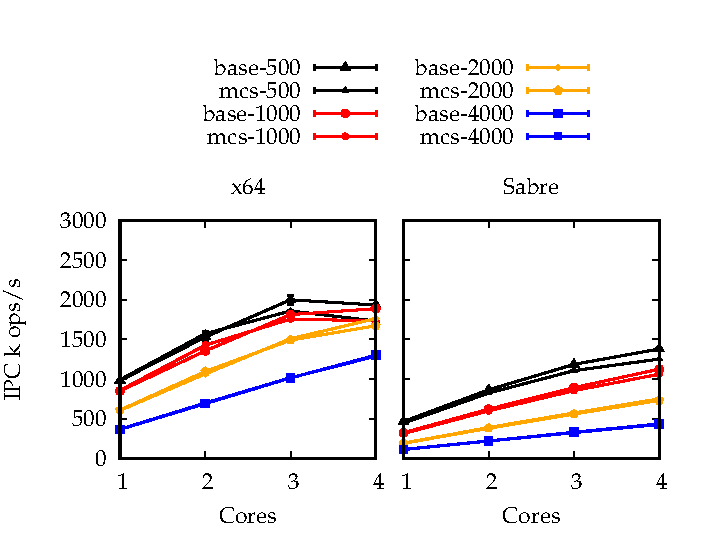
\includegraphics{smp}
    \caption[Results of the multicore IPC throughput benchmark.]{Results of the multicore IPC throughput benchmark, baseline \selfour vs MCS. 
        Each series is named \textit{name-N}, where \textit{name} is \textit{base} and \textit{mcs} for 
        the baseline and MCS kernel respectively, and \textit{N} is the upper
        bound on the number of cycles between each IPC for that series.}
    \label{f:evaluation-smp}
\end{figure}

\subsubsection{Shared server}

We adapt our \gls{AES} case study (\cref{s:server-isolation}) to demonstrate how our MCS model 
applies to multiprocessors. The AES server is configured without a timeout fault handler, and
we run two variants. 

\begin{description}
    \item[Single:] the AES server has a single passive thread, which waits on a single endpoint
        and migrates to the core of the active client over IPC, effectively serialising access to the server.
        Consequently, \cref{f:evaluation-smp-aes} shows there is no gain in throughput when further cores are
        added. 
    \item[Multiple:] the AES server has one passive thread per core, and an endpoint is set up for
        each core, demonstrating a parallel server. Due to minimal bottlenecks in the stateless 
        AES server, this results in near perfect scalability.
\end{description}

\begin{figure}[ht] 
    \centering
    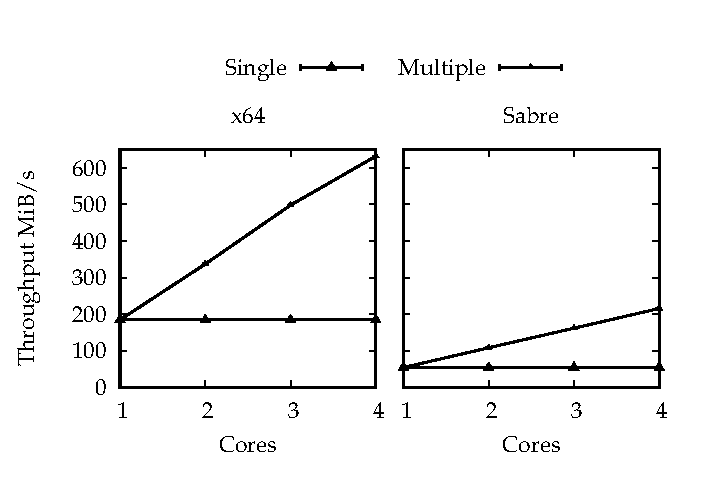
\includegraphics{smp_aes}
    \caption[Results of the AES shared server multicore case study.]{Results of the AES shared server multicore case study. \emph{Single} shows results for a 
        passive server thread migrating between cores to service clients, while \emph{Multiple} has one
        passive server thread per core. For both series, the number of clients is equal to the number of
        cores and each client requests 1MiB of data encrypted. }
    \label{f:evaluation-smp-aes}
\end{figure}

\section{Summary}

All in all, we have demonstrated via micro- and macro- benchmarks that our overheads are
reasonable given the speed of the baseline kernel and the extent of the provided
functionality. 

Through two system benchmarks and one shared-server benchmark, we have shown
that our approach guarantees processor isolation and that threads cannot exceed
their budget allocation via their scheduling context. Additionally, we have
shown that isolation can be achieved in a shared server via a timeout fault
handler and implemented several alternatives for handling such faults,
demonstrating the feasibility of the model. 

Policy freedom is maintained although we provide a fixed-priority scheduling in the kernel, the primitives are provided are sufficient to implement user-level schedulers, 
as demonstrated through the static, mixed-criticality and EDF scheduler
implementations. 

Finally, we have demonstrated that the model works for multiprocessors,
incurring no great scalability penalty over baseline \selfour, 
and showing how passive servers which migrate across cores on \gls{IPC}

\chapter{Conclusion}
\label{chap:conclusion}

Emerging cyber-physical systems represent an opportunity for greater safety, security and 
automation, as they can replace systems where human errors prevail. While humans are excellent at
innovation and creativity, they cannot compete with machines that do not get tired, drunk or
distracted when completing
monotonous, repetitive tasks. Car accidents are overwhelmingly 
caused by human error, measured at 94\% in the US~\citep{Singh_15}, something that self-driving cars can overcome. Autonomous aircraft and other fleet vehicles, smart cities and smart factories hold similar promise. 

As established in \cref{sec:motivation}, in order to practically develop such systems,
they must be mixed-criticality, as certification of all parts of such a system to high-assurance
levels is not feasible. Consequently, mixed-criticality systems require strong temporal isolation
and asymmetric protection between sub-systems of different criticality levels, 
which must also be able to safely share resources.

This thesis has drawn on real-time theory and systems practice to develop core mechanisms required
in a high-assurance, trusted computing base for mixed criticality systems. Importantly, the
mechanisms we have developed do not violate other requirements, like policy-freedom, integrity,
confidentiality, spatial isolation, and security. 

In \cref{chap:model}, we introduced our model for treating time as a first-class resource, and 
defined a minimal set of
mechanisms that can be leveraged to implement temporal isolation between threads, even within shared
servers. Our primitives also allow for more complex, application specific user-level schedulers to
be constructed efficiently, as we demonstrated in the evaluation. Significantly, we provide a
new model for L4 kernels to manage time as a first-class resource, without restricting policy
options including overbooking, 
or requiring specific correlations between the priority of a task and the scheduling model, or
importance of that task. 
We integrate a capability system with the non-fungible resource that is time, without violating our
existing isolation and confidentiality properties, or requiring a heavy performance overhead.
Our mechanisms provide a basic scheduler, which is a critical part of the
trusted computing base, and allow for more system-specific schedulers to be constructed at
user-level. Additionally, we do not force specific
resource-sharing prioritisation policies, but provide mechanisms to allow for their implementation at user-level. 
\clearpage

\section{Contributions}

Specifically, we make the following contributions:

\begin{itemize}
    \item Mechanisms for principled management of time through capabilities to scheduling contexts,
        which are compatible with the fast IPC implementations traditionally used in high-performance
        microkernels, and also compatible with established real-time resource-sharing policies;
    \item an implementation of those mechanisms in the non-preemptible \selfour microkernel, and an
        exploration of how the implementation interacts with the existing kernel model;
    \item an evaluation of the overheads and isolation properties of the implementation, including
        a demonstration of isolation in a shared server through timeout-fault handling;
    \item a design and implementation of many different, user-level timeout-fault handling policies;
    \item and an implementation of a user-level \gls{EDF} scheduler which is as fast as the
        \litmus, in-kernel EDF scheduler, which shows that despite the fixed-priority scheduler
        present in the kernel, other schedulers remain practical;
    \item and a design and implementation of a criticality switch at user-level, which shows that
        criticality is not required to be a kernel-provided property.
\end{itemize}

The implementation is complete, and the verification of this implementation is currently in progress.
Specifications have already been developed by the verification engineering team at Data61, CSIRO,
who are now completing the first-level refinement of the functional correctness proof.
The maximum controlled priority feature has already been verified and merged to the master kernel. 
Verification is beyond the scope of this PhD, although we continue to work closely with
the team to assist in verification. 

This work is part of
the Side-Channel Causal Analysis for Design of Cyber-Physical Security project for the U.S
Department of Homeland Security.

Additionally, during the development of this thesis we have made extensive contributions to the 
\selfour benchmarking suite, testing suite and user-level libraries, all of which provide better 
support for running experiments and building systems on \selfour. 

\section{Future work}

Modern \glspl{CPU} have dynamic frequency scaling and low-power modes in order to reduce energy usage, which
is of high concern in many embedded systems. The implementation as it stands assumes a constant
\gls{CPU} frequency, and all kernel operations are calculated in \gls{CPU} cycles. Frequency scaling
can have undesirable effects on real-time processes: if the period is specified in microseconds, then
converted to cycles and the CPU frequency changes, does the period remain correct? This is a
limitation of our model and promising area for future work.

Although we provide a mechanism for cross-core IPC, where passive threads migrate between processing
cores and active threads remain fixed, there is much more to consider in terms of multicore
scheduling and resource sharing. Our model provides a partitioned, fixed priority scheduler, and 
load balancing can be managed by user level. Further experiments to evaluate the mechanisms for higher-level
multicore scheduling and resource sharing protocols is required. 

Finally, this work does not consider counter-measures for timing-related covert and side channels,
security risks which arise from
shared hardware~\citep{Ge_YCH_18}. \emph{Covert channels} are unintentional, explicit communication
channels which may be used by a malicious sender in a trusted component to leak sensitive data to a receiver
in an untrusted component. Providing a time-source can open a covert channel, where the sender
manipulates timing behaviour through shared architectural structures like caches, and the receiver
uses the time source to observe the behaviour. Shared hardware also presents the risk of
\emph{side channels}, 
where an attacker in an untrusted
component can learn secret information about a trusted component by observing timing behaviour. 
Both attack vectors are risks in mixed-criticality systems, which we do not consider in this
thesis, and merit extensive future work. 

\section{Concluding Remarks}

Original automobiles did not have seat belts, as safety was never a concern. Perhaps one day we
will reflect on human-piloted, high-speed vehicles in the same way. For this future to eventuate, 
cyber-physical systems which combine components of different criticality on shared hardware are essential.
Our work has focused on principled mechanisms for managing time in such systems,
making one significant step towards a future of trustworthy,
safe and secure autonomous systems.

\bigskip
This material is based on research sponsored by the Department of Homeland Security (DHS) Science
and Technology Directorate, Cyber Security Division (DHS S\&T/CSD) BAA HSHQDC-14-R-B00016, and the
Government of United Kingdom of Great Britain and the Government of Canada via contract number
D15PC00223. 


\backmatter
\cleardoublepage
\listoffigures
\clearpage
%\listoftables
%\listofalgorithms
%\addcontentsline{toc}{chapter}{List of algorithms}
\printglossary[type=\acronymtype]
\cleardoublepage
\bibliographystyle{plainnat}
%\bibliographystyle{my-abbrvnat}
%\bibliographystyle{apalike}
\bibliography{references}
\clearpage
\appendix
\addappheadtotoc
\section{Fastpath Performance Analysis}
\input{data/generated/kzm-ipc-perf.inc}
\input{data/generated/sabre-ipc-perf.inc}
\input{data/generated/hikey32-ipc-perf.inc}
\input{data/generated/hikey64-ipc-perf.inc}
\input{data/generated/tx1-ipc-perf.inc}
\input{data/generated/haswell-ipc-perf.inc}

\end{document}
